%======================================================================
% University of Waterloo Thesis Template for LaTeX 
% Last Updated November, 2020 
% by Stephen Carr, IST Client Services, 
% University of Waterloo, 200 University Ave. W., Waterloo, Ontario, Canada
% FOR ASSISTANCE, please send mail to request@uwaterloo.ca

% DISCLAIMER
% To the best of our knowledge, this template satisfies the current uWaterloo thesis requirements.
% However, it is your responsibility to assure that you have met all requirements of the University and your particular department.

% Many thanks for the feedback from many graduates who assisted the development of this template.
% Also note that there are explanatory comments and tips throughout this template.
%======================================================================
% Some important notes on using this template and making it your own...

% The University of Waterloo has required electronic thesis submission since October 2006. 
% See the uWaterloo thesis regulations at
% https://uwaterloo.ca/graduate-studies/thesis.
% This thesis template is geared towards generating a PDF version optimized for viewing on an electronic display, including hyperlinks within the PDF.

% DON'T FORGET TO ADD YOUR OWN NAME AND TITLE in the "hyperref" package configuration below. 
% THIS INFORMATION GETS EMBEDDED IN THE PDF FINAL PDF DOCUMENT.
% You can view the information if you view properties of the PDF document.

% Many faculties/departments also require one or more printed copies. 
% This template attempts to satisfy both types of output. 
% See additional notes below.
% It is based on the standard "book" document class which provides all necessary sectioning structures and allows multi-part theses.

% If you are using this template in Overleaf (cloud-based collaboration service), then it is automatically processed and previewed for you as you edit.

% For people who prefer to install their own LaTeX distributions on their own computers, and process the source files manually, the following notes provide the sequence of tasks:
 
% E.g. to process a thesis called "mythesis.tex" based on this template, run:

% pdflatex mythesis	-- first pass of the pdflatex processor
% bibtex mythesis	-- generates bibliography from .bib data file(s)
% makeindex         -- should be run only if an index is used 
% pdflatex mythesis	-- fixes numbering in cross-references, bibliographic references, glossaries, index, etc.
% pdflatex mythesis	-- it takes a couple of passes to completely process all cross-references

% If you use the recommended LaTeX editor, Texmaker, you would open the mythesis.tex file, then click the PDFLaTeX button. Then run BibTeX (under the Tools menu).
% Then click the PDFLaTeX button two more times. 
% If you have an index as well,you'll need to run MakeIndex from the Tools menu as well, before running pdflatex
% the last two times.

% N.B. The "pdftex" program allows graphics in the following formats to be included with the "\includegraphics" command: PNG, PDF, JPEG, TIFF
% Tip: Generate your figures and photos in the size you want them to appear in your thesis, rather than scaling them with \includegraphics options.
% Tip: Any drawings you do should be in scalable vector graphic formats: SVG, PNG, WMF, EPS and then converted to PNG or PDF, so they are scalable in the final PDF as well.
% Tip: Photographs should be cropped and compressed so as not to be too large.

% To create a PDF output that is optimized for double-sided printing: 
% 1) comment-out the \documentclass statement in the preamble below, and un-comment the second \documentclass line.
% 2) change the value assigned below to the boolean variable "PrintVersion" from " false" to "true".

%======================================================================
%   D O C U M E N T   P R E A M B L E
% Specify the document class, default style attributes, and page dimensions, etc.
% For hyperlinked PDF, suitable for viewing on a computer, use this:
\documentclass[letterpaper,12pt,titlepage,oneside,final]{book}
 
% For PDF, suitable for double-sided printing, change the PrintVersion variable below to "true" and use this \documentclass line instead of the one above:
%\documentclass[letterpaper,12pt,titlepage,openright,twoside,final]{book}

% Some LaTeX commands I define for my own nomenclature.
% If you have to, it's easier to make changes to nomenclature once here than in a million places throughout your thesis!
\newcommand{\package}[1]{\textbf{#1}} % package names in bold text
\newcommand{\cmmd}[1]{\textbackslash\texttt{#1}} % command name in tt font 
\newcommand{\href}[1]{#1} % does nothing, but defines the command so the print-optimized version will ignore \href tags (redefined by hyperref pkg).
%\newcommand{\texorpdfstring}[2]{#1} % does nothing, but defines the command
% Anything defined here may be redefined by packages added below...


\usepackage{tikz}
\usetikzlibrary{shapes.multipart,matrix,positioning,arrows,arrows.meta}
% This package allows if-then-else control structures.
\usepackage{ifthen}
\newboolean{PrintVersion}
\setboolean{PrintVersion}{false}
% CHANGE THIS VALUE TO "true" as necessary, to improve printed results for hard copies by overriding some options of the hyperref package, called below.

%\usepackage{nomencl} % For a nomenclature (optional; available from ctan.org)
\usepackage{amsmath,amssymb,amstext,amsthm} % Lots of math symbols and environments
\usepackage[pdftex]{graphicx} % For including graphics N.B. pdftex graphics driver 

% Hyperlinks make it very easy to navigate an electronic document.
% In addition, this is where you should specify the thesis title and author as they appear in the properties of the PDF document.
% Use the "hyperref" package 
% N.B. HYPERREF MUST BE THE LAST PACKAGE LOADED; ADD ADDITIONAL PKGS ABOVE
\usepackage[pdftex,pagebackref=false]{hyperref} % with basic options
%\usepackage[pdftex,pagebackref=true]{hyperref}
		% N.B. pagebackref=true provides links back from the References to the body text. This can cause trouble for printing.
\hypersetup{
    plainpages=false,       % needed if Roman numbers in frontpages
    unicode=false,          % non-Latin characters in Acrobat’s bookmarks
    pdftoolbar=true,        % show Acrobat’s toolbar?
    pdfmenubar=true,        % show Acrobat’s menu?
    pdffitwindow=false,     % window fit to page when opened
    pdfstartview={FitH},    % fits the width of the page to the window
%    pdftitle={uWaterloo\ LaTeX\ Thesis\ Template},    % title: CHANGE THIS TEXT!
%    pdfauthor={Author},    % author: CHANGE THIS TEXT! and uncomment this line
%    pdfsubject={Subject},  % subject: CHANGE THIS TEXT! and uncomment this line
%    pdfkeywords={keyword1} {key2} {key3}, % list of keywords, and uncomment this line if desired
    pdfnewwindow=true,      % links in new window
    colorlinks=true,        % false: boxed links; true: colored links
    linkcolor=blue,         % color of internal links
    citecolor=green,        % color of links to bibliography
    filecolor=magenta,      % color of file links
    urlcolor=cyan           % color of external links
}
\ifthenelse{\boolean{PrintVersion}}{   % for improved print quality, change some hyperref options
\hypersetup{	% override some previously defined hyperref options
%    colorlinks,%
    citecolor=black,%
    filecolor=black,%
    linkcolor=black,%
    urlcolor=black}
}{} % end of ifthenelse (no else)

\usepackage{diagbox}
\usepackage{wrapfig}
\usepackage[automake,toc,abbreviations]{glossaries-extra} % Exception to the rule of hyperref being the last add-on package
% If glossaries-extra is not in your LaTeX distribution, get it from CTAN (http://ctan.org/pkg/glossaries-extra), 
% although it's supposed to be in both the TeX Live and MikTeX distributions. There are also documentation and 
% installation instructions there.

% Setting up the page margins...
% uWaterloo thesis requirements specify a minimum of 1 inch (72pt) margin at the
% top, bottom, and outside page edges and a 1.125 in. (81pt) gutter margin (on binding side). 
% While this is not an issue for electronic viewing, a PDF may be printed, and so we have the same page layout for both printed and electronic versions, we leave the gutter margin in.
% Set margins to minimum permitted by uWaterloo thesis regulations:
\setlength{\marginparwidth}{0pt} % width of margin notes
% N.B. If margin notes are used, you must adjust \textwidth, \marginparwidth
% and \marginparsep so that the space left between the margin notes and page
% edge is less than 15 mm (0.6 in.)
\setlength{\marginparsep}{0pt} % width of space between body text and margin notes
\setlength{\evensidemargin}{0.125in} % Adds 1/8 in. to binding side of all 
% even-numbered pages when the "twoside" printing option is selected
\setlength{\oddsidemargin}{0.125in} % Adds 1/8 in. to the left of all pages when "oneside" printing is selected, and to the left of all odd-numbered pages when "twoside" printing is selected
\setlength{\textwidth}{6.375in} % assuming US letter paper (8.5 in. x 11 in.) and side margins as above
\raggedbottom

% The following statement specifies the amount of space between paragraphs. Other reasonable specifications are \bigskipamount and \smallskipamount.
\setlength{\parskip}{\medskipamount}

% The following statement controls the line spacing.  
% The default spacing corresponds to good typographic conventions and only slight changes (e.g., perhaps "1.2"), if any, should be made.
\renewcommand{\baselinestretch}{1} % this is the default line space setting

% By default, each chapter will start on a recto (right-hand side) page.
% We also force each section of the front pages to start on a recto page by inserting \cleardoublepage commands.
% In many cases, this will require that the verso (left-hand) page be blank, and while it should be counted, a page number should not be printed.
% The following statements ensure a page number is not printed on an otherwise blank verso page.
\let\origdoublepage\cleardoublepage
\newcommand{\clearemptydoublepage}{%
  \clearpage{\pagestyle{empty}\origdoublepage}}
\let\cleardoublepage\clearemptydoublepage

% Define Glossary terms (This is properly done here, in the preamble and could also be \input{} from a separate file...)
% Main glossary entries -- definitions of relevant terminology
\newglossaryentry{computer}
{
name=computer,
description={A programmable machine that receives input data,
               stores and manipulates the data, and provides
               formatted output}
}

% Nomenclature glossary entries -- New definitions, or unusual terminology
\newglossary*{nomenclature}{Nomenclature}
\newglossaryentry{dingledorf}
{
type=nomenclature,
name=dingledorf,
description={A person of supposed average intelligence who makes incredibly brainless misjudgments}
}

% List of Abbreviations (abbreviations type is built in to the glossaries-extra package)
\newabbreviation{aaaaz}{AAAAZ}{American Association of Amateur Astronomers and Zoologists}

% List of Symbols
\newglossary*{symbols}{List of Symbols}
\newglossaryentry{rvec}
{
name={$\mathbf{v}$},
sort={label},
type=symbols,
description={Random vector: a location in n-dimensional Cartesian space, where each dimensional component is determined by a random process}
}
\makeglossaries

\newtheorem{lemma}{Lemma}
%======================================================================
%   L O G I C A L    D O C U M E N T
% The logical document contains the main content of your thesis.
% Being a large document, it is a good idea to divide your thesis into several files, each one containing one chapter or other significant chunk of content, so you can easily shuffle things around later if desired.
%======================================================================
\begin{document}

%----------------------------------------------------------------------
% FRONT MATERIAL
% title page,declaration, borrowers' page, abstract, acknowledgements,
% dedication, table of contents, list of tables, list of figures, nomenclature, etc.
%----------------------------------------------------------------------
% T I T L E   P A G E
% -------------------
% Last updated October 23, 2020, by Stephen Carr, IST-Client Services
% The title page is counted as page `i' but we need to suppress the
% page number. Also, we don't want any headers or footers.
\pagestyle{empty}
\pagenumbering{roman}

% The contents of the title page are specified in the "titlepage"
% environment.
\begin{titlepage}
        \begin{center}
        \vspace*{1.0cm}

        \Huge
        {\bf Coupled models of structured contagious processes}

        \vspace*{1.0cm}

        \normalsize
        by \\

        \vspace*{1.0cm}

        \Large
        Peter C. Jentsch \\

        \vspace*{3.0cm}

        \normalsize
        A thesis \\
        presented to the University of Waterloo \\ 
        in fulfillment of the \\
        thesis requirement for the degree of \\
        Doctor of Philosophy \\
        in \\
        Applied Mathematics \\

        \vspace*{2.0cm}

        Waterloo, Ontario, Canada, 2021 \\

        \vspace*{1.0cm}

        \copyright\ Peter C. Jentsch \\
        \end{center}
\end{titlepage}

% The rest of the front pages should contain no headers and be numbered using Roman numerals starting with `ii'
\pagestyle{plain}
\setcounter{page}{2}

\cleardoublepage % Ends the current page and causes all figures and tables that have so far appeared in the input to be printed.
% In a two-sided printing style, it also makes the next page a right-hand (odd-numbered) page, producing a blank page if necessary.

 
% E X A M I N I N G   C O M M I T T E E (Required for Ph.D. theses only)
% Remove or comment out the lines below to remove this page
\begin{center}\textbf{Examining Committee Membership}\end{center}
  \noindent
The following served on the Examining Committee for this thesis. The decision of the Examining Committee is by majority vote.
  \bigskip
  
  \noindent
\begin{tabbing}
Internal-External Member: \=  \kill % using longest text to define tab length
External Examiner: \>  Bruce Bruce \\ 
\> Professor, Dept. of Philosophy of Zoology, University of Wallamaloo \\
\end{tabbing} 
  \bigskip
  
  \noindent
\begin{tabbing}
Internal-External Member: \=  \kill % using longest text to define tab length
Supervisors: \> Chris T. Bauch \\
\> Professor, Department of Applied Mathematics, University of Waterloo \\
\> Madhur Anand \\
\> Professor, School of Environmental Sciences, University of Guelph \\
\end{tabbing}
  \bigskip
  
  \noindent
  \begin{tabbing}
Internal-External Member: \=  \kill % using longest text to define tab length
Internal Members: \> Sue Ann Campbell \\
\> Professor, Department of Applied Mathematics, University of Waterloo \\ 
\> Zoran Miskovic  \\
\> Professor, Department of Applied Mathematics, University of Waterloo \\
\end{tabbing}
  \bigskip
  
  \noindent
\begin{tabbing}
Internal-External Member: \=  \kill % using longest text to define tab length
Internal-External Member: \> Meta Meta \\
\> Professor, Dept. of Philosophy, University of Waterloo \\
\end{tabbing}
  \bigskip
  
  \noindent
\begin{tabbing}
Internal-External Member: \=  \kill % using longest text to define tab length
Other Member(s): \> Leeping Fang \\
\> Professor, Dept. of Fine Art, University of Waterloo \\
\end{tabbing}

\cleardoublepage

% D E C L A R A T I O N   P A G E
% -------------------------------
  % The following is a sample Delaration Page as provided by the GSO
  % December 13th, 2006.  It is designed for an electronic thesis.
 \begin{center}\textbf{Author's Declaration}\end{center}
  
 \noindent
This thesis has entirely been authored or co-authored by me. This is a true copy of the thesis, including any required final revisions, as accepted by my examiners.

  \bigskip
  
  \noindent
I understand that my thesis may be made electronically available to the public.

\cleardoublepage

% Contributions
% -------------------------------
  % The following is a sample Delaration Page as provided by the GSO
  % December 13th, 2006.  It is designed for an electronic thesis.
  \begin{center}\textbf{Statement of Contributions}\end{center}
  
  \begin{itemize}
    
   \item Chapter \ref{ch1}: MA and CTB conceptualized the study. All authors designed the model. PCJ developed and analysed the model and generated figures. PCJ and CTB wrote the first draft of the manuscript and accessed and verified the data. All authors revised the manuscript critically for important intellectual content, and read and approved the final version of the manuscript. All authors had full access to all the data in the study, and the corresponding author had final responsibility for the decision to submit for publication. The contents of this chapter are based on the corresponding article published in \textit{Lancet Infectious Diseases} \cite{jentsch2021prioritising}.
   
   \item Chapter \ref{ch2}: Conceptualization by DY, MA, data curation by PCJ, DY, formal analysis by PCJ, funding acquisition by CTB, DY, MA, investigation by PCJ, CTB, DY, MA. Methodology by PCJ, CTB, DY, MA. Project administration by PCJ, CTB, DY, MA. Resources by CTB, DY, MA. Software written by PCJ. Supervision by CTB, DY, MA, validation by PCJ, CTB, DY, MA, visualization by PCJ, CTB. Original draft written by PCJ. Review & editing by PCJ, CTB, DY, MA. The contents of this chapter are based on the corresponding article published in \textit{PLoS One} \cite{jentsch2020go}.

   
   \item Chapter \ref{ch3}: The work in this chapter is based upon a manuscript under review at the \textit{Journal of Theoretical Ecology}. All authors conceived ideas for the study. PCJ designed and coded the model, performed
   analyses, created figures, and drafted the manuscript. All authors revised the manuscript.
   

  \end{itemize}
 \cleardoublepage
 
% A B S T R A C T
% ---------------

\begin{center}\textbf{Abstract}\end{center}

% In 2021, the biosphere of the earth has been almost entirely eradicated and replaced by a thin facsimile. Many of the ecosystems that once spanned the globe have been reduced to skeletons, supported by the scaffolding of dwindling state environmental agency budgets. 

Models of infectious processes are a common feature in the landscape of applied mathematics. Is is very rare that these processes are isolated from other significant dynamics in nature, and therefore we can incorporate some of the complexity inherent in real systems by coupling infections to major features of the ecosystems they inhabit. Infectious processes can take many forms, but in this thesis we consider three: the COVID-19 pandemic, the invasion of eastern North American forests by wood-borne pests, and the outbreak cycles of an endemic forest pest. The first chapter covers a model of Sars-CoV-2 in a structured population, coupled with a replicator equation representing sentiment towards the use of non-pharmaceutical interventions. We use this model to compare the efficacy of vulnerable-first and transmission-preventing age structured vaccination strategies. The buildup of natural immunity in a population combined with a low vaccination supply, is shown to cause a transmission-preventing vaccination strategy to be more effective. The second chapter considers a model of forest pest transport over an empirically-derived network of forest patches in eastern Canada. Since these pests can frequently be spread long distances by wood transport, we couple this model to the sentiment of local populations towards avoiding firewood transport from outside their area. Three possible countermeasures to the spread of the invasive pest are compared: social incentives, direct interception of infested firewood, and quarantine of patches. The level of effort needed to significantly reduce forest damage with any of these methods is substantial and unlikely to be implemented. The final chapter extends a model of mountain pine beetle (MPB) in western north american pine forests to incorporate tree mortality due to wildfire. We find that wildfire acts as a disturbance that increases the heterogeneity in age structure, and therefore is able to increase the resilience of the forest to outbreaks of MPB. A targeted thinning procedure aimed specifically at increasing heterogeneity in the forest age structure is proposed and shown to be highly effective at reducing the severity of outbreak. The effectiveness of targeted thinning in the manner described further emphasizes the importance of heterogeneity in forest stand structure.



\cleardoublepage

% A C K N O W L E D G E M E N T S
% -------------------------------

\begin{center}\textbf{Acknowledgements}\end{center}

I would like to thank the following people for making this thesis possible.

\begin{itemize}
\item My supervisors, Dr. Chris Bauch and Dr. Madhur Anand, for their endless support, understanding, and insight throughout my graduate and undergraduate career.  
  
\item Dr. Sue Ann Campbell and Zoran Miskovic for being on my PhD committee.

\item Dr. Denys Yemshanov for his patience and mentorship on things forest-related. 

\item Dr. Mark Penney for the great conversations, collaboration, and opportunity to write an agent-based model in the last six months of my PhD.

\item Dr. Chrystopher Nehaniv for the opportunities to think and present about topics almost completely different from those in this thesis. 

\item My friends in the Bauch Lab, the applied mathematics department, and outside the university for the time spent not working, and many victorious bar trivia nights.
 
\item Samantha Landry and Emylee Todd for reading and editing the early drafts of this thesis.

\item My mom, dad, and siblings, for their support, encouragement, and not asking "so when are you gonna graduate" too often.  
\end{itemize}

 
\cleardoublepage

% D E D I C A T I O N
% -------------------

\begin{center}\textbf{Dedication}\end{center}

For Emmy, Max, Sam, and the friends that have helped me get through the past 5 years.


\cleardoublepage

% T A B L E   O F   C O N T E N T S
% ---------------------------------
\renewcommand\contentsname{Table of Contents}
\tableofcontents
\cleardoublepage
\phantomsection    % allows hyperref to link to the correct page

% L I S T   O F   F I G U R E S
% -----------------------------
\addcontentsline{toc}{chapter}{List of Figures}
\listoffigures
\cleardoublepage
\phantomsection		% allows hyperref to link to the correct page

% L I S T   O F   T A B L E S
% ---------------------------
\addcontentsline{toc}{chapter}{List of Tables}
\listoftables
\cleardoublepage
\phantomsection		% allows hyperref to link to the correct page

% Change page numbering back to Arabic numerals
\pagenumbering{arabic}

 

%----------------------------------------------------------------------
% MAIN BODY
% We suggest using a separate file for each chapter of your thesis.
% Start each chapter file with the \chapter command.
% Only use \documentclass or \begin{document} and \end{document} commands in this master document.
% Tip: Putting each sentence on a new line is a way to simplify later editing.
%----------------------------------------------------------------------
\chapter{Introduction}

I am writing this introduction sitting in my living room in Kitchener, Ontario, staring at the dead ash tree which overlooks the empty lots that border my home. Ash trees (\textit{Fraxinus} sp.) were a common street tree in the eastern Unites States and Canada, but in the past two decades, the emerald ash borer (\textit{Agrilus planipennis}, EAB) has spread throughout the region, killing about 99\% of the Ash trees in the regions they invade \cite{nrcaneab,herms2014emerald}. Once a prominent feature of deciduous woodlands in this area, \textit{Fraxinus} is now limited to rare pockets that have escaped the insect, and seedlings, still too small to be infested. This narrative is a familar one. The american chestnut (\texit{Castanea dentata}) was once a major part of the eastern american landscape, an important source of lumber, and food. It was almost completely wiped out as the chestnut blight (\textit{Cryphonectria parasitica}) spread throughout eastern north america in the 19th and 20th centuries. Infectious agents in this way shape the landscapes we inhabit and the ecosytems we exist within. Of course, infectious agents are not limited to arboreal hosts: I have been in my living room staring at this dead ash tree for the past year, sheltering from the global Covid-19 pandemic. 

Pandemics, such as the various waves of the Black Death, the 1918 influenza pandemic, the HIV/AIDS pandemic, and the current Covid-19 pandemic, have irreversibly shaped our culture. Endemic infectious disease, was until very recently, a massive driving force in the formation of human societies everywhere. Only in the past century have some parts of the world been able to escape the spectre of endemic disease such as malaria, polio, influenza, and measles. John Snow is considered to be one of the first epidemiologists, for his study of London Cholera outbreaks \cite{snow1855mode, brauer2019mathematical}. However, during recent outbreaks of infectious agents, compartmental models are one of the main tools used to forecast outcomes and mitigation stragies \cite{brauer2008compartmental}. Due to the ongoing pandemic, the general public is probably more aware than ever before of these models.

Compartmental models for the spread of infectious diseases are usually considered to have been introduced to the field by public health researchers, such as Hamer, Kermack and McKendrick \cite{hamer1906epidemic, kermack1927contribution, brauer2019mathematical,edelstein2005mathematical}. This class of models divides the population into homogenous compartments, and describe the rate of movement between these compartments. The quintessential compartmental model is the SIR model (equations \ref{SIR}), so-called for it's division of a population into Susceptible (the $S(t)$ variable), Infected (the $I(t)$ variable), and Recovered (the $R(t)$ variable) compartments.

\begin{eqnarray}
    \frac{dS}{dt} = -\beta S I  \\
    \frac{dI}{dt} = \beta S I - \gamma I\\
    \frac{dR}{dt} = \gamma I\\
    \label{SIR}
\end{eqnarray}

The SIR model describes a population undergoing an infection that confers complete immunity after one has been infected, under a great number of simplying assumptions: each compartment is totally homogenous, the likelihood of infection is proportional to the number of individuals in each compartment, and the probability that an individual recovers is constant per unit time. From the initial work on these models, the invention of computers has allowed researchers to get useful results from even the most complex elaborations on this theme. The assumption of homogeneity is a major drawback of the SIR model, so a common extension to this model is to add more structure, usually through furthur subdivision of the compartments. 

\section{Sars-Cov-2}

Compartmental models have been invaluable in modeling the spread of Sars-CoV-2 \cite{thompson2020epidemiological}. It is difficult to overstate the damage and loss of life that the ongoing COVID-19 pandemic has caused or exacerbated in the past year \cite{miller2020disease,who2021impact}. The first human case of Sars-CoV-2 occurred in late 2019 in central China, almost certainly transmitted from an animal host, very likely a bat \cite{andersen2020proximal,rasmussen2021origins,zhu2020novel}. The virus soon spread throughout the world, and was declared a pandemic by the World Health Organization (WHO), on March 11th, 2020 \cite{who2020announces}. In the intervening months, people around the world have endured various levels of non-pharmeceutical interventions (NPIs), from comprehensive quarantine procedures (in e.g. New Zealand, South Korea, Singapore, Vietnam) to almost nothing at all (United States, Sweden). In the outcomes of the aforementioned countries, empirical research, and modelling studies, NPIs have been shown to be an effective method for the control of Covid-19 \cite{anderson2020estimating,flaxman2020estimating,ferguson2020report,demirguc2020sooner}. 



\section{Imitation dynamics}


The demonstrated effectiveness of NPIs in some countries implies that the immense morbidity and mortality over the past year is not simply a natural disaster, but a humanitarian one. Since our survival depends on our ability to construct a world in which people are incentivized to centre the well-being of others, any attempt to model human outcomes of the pandemic should also attempt to model the incentive strucutures we operate within. A very simple model for this is the game theoretical one \cite{andrews2015disease,jentsch2018spatial}. In this framework, we assume that NPI usage is a prisoners dilemma in that everyone either cooperates or defects with the practice of using NPIs, and the decision to defect to cooperate is based on a combination of the percieved payoff to do so, and the influence of the rest of the population. Table \ref{prisonersdilemma} shows the payoff matrix of this 2-player game. Of course in real life, we are all playing this game, all the time, with everyone. 
\begin{figure}
    \begin{tabular}{ |c|c| c| } \hline
        \diagbox[width = 7em, height = 2em]{P1}{P2} &use NPI& don't use NPI   \\ \hline
        use NPI & \diagbox[width = 13em, height = 8em]{low risk,\\ NPIs unpleasant}{low risk,\\ NPIs unpleasant} &  \diagbox[width = 13em, height = 8em]{med risk,\\ NPIs unpleasant} {med risk}\\ \hline 
        don't use NPI & \diagbox[width = 13em, height = 8em]{med risk}{med risk,\\ NPIs unpleasant} &  \diagbox[width = 13em, height = 8em]{high risk}{high risk}   \\ \hline
    \end{tabular}
    \caption{NPI adoption as a two-player game (between P1 and P2)}
    \label{prisonersdilemma}
\end{figure}


The simplest way to approximate the time evolution of a such a game is with the one-dimensional replicator equation, which approximates these dynamics in terms of the population average \cite{hofbauer1998evolutionary}. Specifically, we introduce a variable $x(t)$ which represents the fraction of people adopting a strategy, then the replicator equation \ref{replicator} gives the time-evolution of $x(t)$ in terms of the payoff for cooperating over defecting, $p(x,t)$. We see immediately that this equation, disregarding $p(x,t) = 0$, has two steady states: $x = 1$ and $x = 0$. Given $p(x,t)$ constant, the population will approach whichever point it is initially closer to. 

\begin{equation}
    \frac{dx}{dt} = \sigma x(1 - x)p(x,t) 
    \label{replicator}
\end{equation}


This formulation has been also used to model vaccination sentiment in a variety of scenarios \cite{oraby2014influence,bauch2004vaccination,bauch2005imitation,bauch2012evolutionary}. In this context, "cooperation" refers to the strategy of getting a widely-available vaccine, and the cooperation payoff function is usually of the form in equation \ref{vacpayoff}. The population is assumed to have a constant payoff to avoid vaccination (in many cases, just due to inconvenience), and a payoff to vaccinate proportional to $I$, the prevalence of infection in the model. 

\begin{equation}
    p(x,t) = - c + \rho I
    \label{vacpayoff}
\end{equation}


A prisoners dilemma formulation and model based upon equation \ref{replicator} coupled to an application-specific model (in the above case, disease dynamics), can also be applied to human-environment models in ecology. In particular, it has been used to model conservation responses coupled to ecosystem dynamics in contexts such as forest-grassland mosaics \cite{innes2013impact,henderson2016alternative}, global climate \cite{bury2019charting}, coral reefs \cite{thampi2018socio}, argicultural land use \cite{gooding2018forest}. I will focus on the application of imitation dynamics to forest pest transport, and the use of NPIs in the context of the Covid-19 pandemic.


\section{Forest pests in eastern North America}

The term "forest pests" covers a broad range of infectious agents that are reponsible for forest tree damage and mortality. Major invading forest pests in eastern North America include: the Asian longhorned beetle (\textit{Anoplophora glabripennis}), the butternut canker (\textit{Ophiognomonia clavigignenti-juglandacearum}), the gypsy moth (\textit{Lymantria dispar dispar}), dutch elm disease \textit{Ophiostoma ulmi}, and the aforementioned EAB. Together, these non-native pests kill 5.53 teragrams of carbon worth of trees each year, on an order of magnitude comparable to forest fires on the continent \cite{fei2019biomass}. Non-native insect invaders are usually introduced by accident. The majority of recently species are a result of careless global trade, with new individuals arriving in lumber, live plants, or similar goods \cite{brockerhoff2017ecology}. Models for predicting the spread of these insects are often inspired by models for infectious diseases in humans. While research in mathematical ecology generally uses the related lotka-volterra model for host-parasitoid dynamics, SIR models can be a natural choice because they focus on the time-evolution of the host populations, which is often the more useful quantity \cite{edelstein2005mathematical}. In this thesis we will expand on the model of Barlow et al \cite{barlow2014modelling}, which couples an SIR-style model of an invading species assisted by human transport of firewood.

\section{Western Pine forest ecosystems}





%just generally describe western pine forests
%pine beetles are sort of similar to other forest pests, except endemic I guess lol

%heavily seasonal dynamics suggests a discrete model?? talk about this here?



% \addcontentsline{toc}{chapter}{Introduction} \markboth{INTRODUCTION}{} \lipsum[1-5]

% The growth of an organism within a population over time is a common subject of research in ecology and the natural sciences. Some of the first dynamic models of this process were created by Lokta and Volterra in the early 20th century \cite{lotka1920analytical,volterra1928variations,lotka1925elements}. The lotka-volterra model (Equations \ref{lotkavolterra}) describes the time-evolution of two populations, a predator and a prey, under many simplifying assumptions. Namely, this model assuming that prey grows exponentially in the abscence of a predator, and that populations are completely homogenous in space, the growth rate of predators depends entirely on the population of prey, and that population sizes are the only factor governing the rate of predation.


% \begin{eqnarray}
    %     \frac{dx}{dt} = \alpha x - \beta x y \\
%     \frac{dy}{dt} = \gamma x y - \delta y\\
%     \label{lotkavolterra}
% \end{eqnarray}

% The spread of a 
\chapter{Prioritising COVID-19 vaccination in changing social and epidemiological landscapes: a mathematical modelling study}
\label{ch1}
\let\thefootnote\relax\footnote{This chapter is based on the paper: Jentsch, Peter C., Madhur Anand, and Chris T. Bauch. "Prioritising COVID-19 vaccination in changing social and epidemiological landscapes: a mathematical modelling study." The Lancet Infectious Diseases (2021).}
\begin{abstract}
  During the COVID-19 pandemic, authorities must decide which groups to prioritise for vaccination in a shifting social–epidemiological landscape in which the success of large-scale non-pharmaceutical interventions requires broad social acceptance. We aimed to compare projected COVID-19 mortality under four different strategies for the prioritisation of SARS-CoV-2 vaccines. We developed a coupled social–epidemiological model of SARS-CoV-2 transmission in which social and epidemiological dynamics interact with one another. We modelled how population adherence to non-pharmaceutical interventions responds to case incidence. In the model, schools and workplaces are also closed and reopened on the basis of reported cases. The model was parameterised with data on COVID-19 cases and mortality, SARS-CoV-2 seroprevalence, population mobility, and demography from Ontario, Canada (population 14.5 million). Disease progression parameters came from the SARS-CoV-2 epidemiological literature. We assumed a vaccine with 75\% efficacy against disease and transmissibility. We compared vaccinating those aged 60 years and older first (oldest-first strategy), vaccinating those younger than 20 years first (youngest-first strategy), vaccinating uniformly by age (uniform strategy), and a novel contact-based strategy. The latter three strategies interrupt transmission, whereas the first targets a vulnerable group to reduce disease. Vaccination rates ranged from 0.5\% to 5\% of the population per week, beginning on either Jan 1 or Sept 1, 2021. Case notifications, non-pharmaceutical intervention adherence, and lockdown undergo successive waves that interact with the timing of the vaccine programme to determine the relative effectiveness of the four strategies. Transmission-interrupting strategies become relatively more effective with time as herd immunity builds. The model predicts that, in the absence of vaccination, 72000 deaths (95\% credible interval 40000–122000) would occur in Ontario from Jan 1, 2021, to March 14, 2025, and at a vaccination rate of 1.5\% of the population per week, the oldest-first strategy would reduce COVID-19 mortality by 90.8\% on average (followed by 89.5\% in the uniform, 88.9\% in the contact-based, and 88.2\% in the youngest-first strategies). 60000 deaths (31000–108000) would occur from Sept 1, 2021, to March 14, 2025, in the absence of vaccination, and the contact-based strategy would reduce COVID-19 mortality by 92.6\% on average (followed by 92.1\% in the uniform, 91.0\% in the oldest-first, and 88.3\% in the youngest-first strategies) at a vaccination rate of 1.5\% of the population per week.Interpretation The most effective vaccination strategy for reducing mortality due to COVID-19 depends on the time course of the pandemic in the population. For later vaccination start dates, use of SARS-CoV-2 vaccines to interrupt transmission might prevent more deaths than prioritising vulnerable age groups.

\end{abstract}


\section{Introduction}


The COVID-19 pandemic has imposed a massive global health burden as waves of infection to move through populations around the world \cite{miller2020disease}.  Both empirical analyses and mathematical models conclude that non-pharmaceutical interventionsn (NPIs) are effective in reducing COVID-19 case incidence \cite{anderson2020estimating,peak2020individual,tuite2020mathematical}.  However, pharmaceutical interventions are highly desirable given the socio-economic costs of lockdown and physical distancing.  Hence, dozens of vaccines are  in development \cite{lurie2020developing}, and  model-based analyses are exploring the question of which groups should get the COVID-19 vaccine first \cite{bubar2020model,hoyt2020vaccine}.  


When vaccines become available, we will face a very different epidemiological landscape from the early pandemic. Many populations will already have experienced one or more waves of COVID-19.  As a result of natural immunity, the effective reproduction number $R_{eff}$ (the average number of secondary infections produced per infected person) will be reduced from its original value of approximately $R_0 = 2.2$ in the absence of pre-existing immunity \cite{hilton2020estimation}. Epidemiological theory tells us that as $R$ (or $R_0$) decline toward 1, the indirect benefits of transmission-blocking vaccines become stronger.  For instance, if $R_{eff} \approx 1.5$, such as for seasonal influenza, only an estimated $33 \%$ percent of the population needs immunity for transmission to die out in a homogeneously mixing population  \cite{anderson1992infectious,dushoff2007vaccinating}.  This effect was evidenced by the strong suppression of influenza incidence in Australia in Spring 2020 due to NPIs targeted against COVID-19 \cite{aussie2020}. 

This effect has stimulated a literature comparing the vaccination of groups that are responsible for most transmission to vaccination of groups that are vulnerable to serious complications from the infection. Natural immunity to SARS-CoV-2 will likely continue to rise in many populations on account of further infection waves. Given these likely changes to the epidemiological landscape before the vaccine becomes available, we suggest this question is worthy of investigation in the context of COVID-19. 


The social landscape will also look very different when vaccines become available and this aspect is crucial to understanding the pandemic. Scalable non-pharmaceutical interventions (NPIs) like physical distancing, hand-washing and masks are often one of the few available interventions when a novel pathogen emerges. Flattening the COVID-19 epidemic curve was possible due to a sufficient response by populations willing to adhere to public health recommendations. Therefore, pandemic waves are not simply imposed on populations -- they are a creation of the population response to the pathogen. They exemplify coupled socio-epidemiological systems exhibiting two-way feedback between disease dynamics and behavioural dynamics interact with one another \cite{pedro2020conditions}.

Approaches to modelling coupled social-epidemiological dynamics vary\cite{reluga2010game,salathe2008effect,funk2009spread,verelst2016behavioural,funk2010modelling}.  Some models have used evolutionary game theory to model this two-way feedback in a variety of coupled human-environment systems \cite{pedro2020conditions,bauch2005imitation,innes2013impact,bury2019charting,amaral2020epidemiological,zhao2020imitation,alam2020based}.  Evolutionary game theory captures how individuals learn social behaviours from others while weighing risks and benefits of different choices. In this framework, individuals who do not adopt NPIs can “free-ride” on the benefits of reduced transmission generated by individuals who do adopt NPIs \cite{reluga2010game}. 

Here, our objective is to compare projected COVID-19 mortality under four strategies for the prioritisation of COVID-19 vaccines: older individuals first, children first, uniform allocation, and a novel strategy based on the contact structure of the population. We use an age-structured model of SARS-CoV-2 transmission, including evolutionary game theory to model population adherence to NPIs and changes to mobility patterns.  We use scenario and sensitivity analysis to identify how strategy effectiveness responds to possible changes in the social-epidemiological landscape that may occur before and after vaccines become available.  

\section{Model Overview}

\subsection{Structure and parameterisation}

We developed an age-structured SEPAIR model (Susceptible, Exposed, Presymptomatic, Asymptomatic, Symptomatic, Removed) with ages in 5-year increments. Upon infection, individuals enter a latent period where they are infected but not yet infectious (“Exposed”).  After the latent period, individuals become presymptomatically infectious, and then either symptomatically or asymptomatically infectious, before finally entering the Removed compartment when their infectiousness ends. We did not model testing or contact tracing explicitly, although we assume infected individuals are ascertained at some rate. Transmission occurs through an age-specific contact matrix, susceptibility to infection is age-specific, and we include seasonality due to changes in the contact patterns throughout the year.  To infer model parameters, we fitted the model to Ontario COVID-19 case notifications stratified by age and time, Ontario seroprevalence data, and Ontario mobility data.  Use of seroprevalence data ensured that our estimates of transmission were not biased by case under-reporting. Remaining model parameter values were fixed using Ontario demographic and mortality data, and literature on COVID-19 serial interval and incubation periods. The system of differential equations comprising our model is solved numerically with DifferentialEquations.jl in the Julia language \cite{rackauckas2017differentialequations}.

Both schools and workplaces are closed when the number of ascertained active cases surpasses 50\%, 100\%, 150\%, 200\%, or 250\% of the peak ascertained active cases that occurred during the first wave (the “shutdown threshold”, T), and are re-opened again when cases fall below that threshold. Individuals interact with other individuals at a specified rate and switch between adherence and non-adherence to NPIs, including mobility restrictions, by comparing the cost of practicing NPIs against the cost of not practicing NPIs and thereby being subject to an increased risk of infection according to the prevalence of ascertained cases.  Both school and workplace closure and population level of adherence to NPIs reduce transmission according to a specified efficacy. 



\subsection{Model Equations}
 
Transmission dynamics are given by an SEPAIR model, modified to take population adherence to NPIs and school/workplace closure into account, and divided into age classes $i \in [1,16]$, where each age class contains a 5 year cohort, except for the oldest age group which comprises the ages $75$ and over. The model equations are:

\textcolor{black}{\begin{eqnarray}
\frac{dS^1_i}{dt} &= & S^1_i \left(- r \rho_i  \xi(t) \sum_{j=1}^{16} C_{ij}(t) \left(\frac{I_{s_j} + I_{a_j} + P_j}{N_j}\right) - \tau\right) \label{S1eqn} \\
\frac{dS^2_i}{dt} &= & S^2_i \left(- r \rho_i  \xi(t) \sum_{j=1}^{16} C_{ij}(t) \left(\frac{I_{s_j} + I_{a_j}+ P_j}{N_j}\right)  - \tau \right)  \label{S2eqn} \\
\frac{dE_i}{dt} &= &  (S^1_i + S^2_i) \left(r_i  \xi(t) \sum_{j=1}^{16} C_{ij}(t) \left(\frac{I_{s_j} + I_{a_j}+ P_j}{N_j}\right) - \sigma_0 E_i + \tau \right) \label{Eeqn} \\
\frac{dP_i}{dt} &= & \sigma_0 E_i - \sigma_1 P_i \label{Peqn} \\
\frac{dI_{a_i}}{dt} &= & \eta \sigma_1 E_i - \gamma_a I_{a_i}\label{Ieqn} \\
\frac{dI_{s_i}}{dt} &= & (1 - \eta) \sigma_1 E_i - \gamma_s I_{s_i} \label{Ieqn} \\
\frac{dR_i}{dt} &= & \gamma_a I_{a_i} + \gamma_s I_{s_i}  \label{Reqn} \\
\frac{dD_i}{dt} &= & \Omega(D(t)) \label{Deqn}
\end{eqnarray}}

where $\xi(t) = \left[1 + s \sin\left(\frac{2 \pi}{365} (t - \phi) - \frac{\pi}{2}\right)\right]$ determines the seasonally varying transmission rate with phase $\phi$ and amplitute $s$.

\noindent Parameter values are defined in Table \ref{tab:params}. The vaccination dynamics are an impulsive process applied each day, described below. $S^{1}_i$ is the number of unvaccinated susceptible individuals in age group $i$, and $S^{2}_i$ is the number of susceptible individuals in age group $i$ who have received a standard two dose course of vaccination but were not immunized. $E_i(t)$ is the number of exposed but not yet infectious individuals in age group $i$ (\textcolor{black}{i.e., individuals in the latent period}). $I_{a_i}(t)$ is the number of asymptomatic infectious individuals in age group $i$ and $I_{s_i}(t)$ is the number of symptomatic infectious individuals in age group $i$. $R_i(t)$ is the number of Removed (recovered, vaccinated, and deceased) individuals in compartment $i$.

The variable $D(t) \in [0,1]$ in the model equation $dD(t)/dt = \Omega(D(t))$ represents the public health authority's reaction to the prevalence of ascertained cases and it evolves according to: 
\begin{eqnarray}
  \Omega(D(t)) =  \left\{
\begin{array}{ll}
    k_1 (1 - D(t)) &  \sum_{i=1}^{16}\alpha_i(I_{a_i} + I_{s_i}) > T\\
    - k_2 D(t) & \sum_{i=1}^{16}\alpha_i(I_{a_i} + I_{s_i}) \leq T
\end{array} 
\right. 
\end{eqnarray}
This represents closure being triggered when ascertained cases exceed a threshold $T$, and being lifted when cases drop below that threshold again. 

The proportion $x$ of individuals who practice NPIs such as mask wearing, handwashing, and physical distancing, starts off at $x(0)=0.01$ and evolves as: 
\begin{eqnarray}
\frac{dx}{dt} &= &\kappa x (1-x) \left(\frac{\sum_{i=1}^{16}\alpha_i(I_{a_i} + I_{s_i})}{\sum_{i=1}^{16} N_i} - c x\right) + p_{ul}(1-2 x) 
\label{xeqn_new}
\end{eqnarray}
where $\kappa$ is the social learning rate, $c$ is the incentive to not practice NPIs, and $\alpha_i$ is the fraction of total cases ($I_a + I_s$) that are reported, also known as the ascertainment rate.  The $p_{ul}$ term is a phenomenological term that represents the effects of social heterogeneity and influence from external populations that prevents the system from remaining arbitrarily close to $x=0$ or $x=1$ for unrealistic periods of time.  These equations describe a population where individual sample other individuals at some time rate and switch between adherence and non-adherence to NPIs with a probability proportional to the expected gain in utility $\sum_{i=1}^{16}\alpha_i(I_{a_i} + I_{s_i}) - c x$. We refer the reader to existing literature for details on the derivation of this equation \cite{bauch2005imitation,innes2013impact,thampi2018socio,bauch2012evolutionary,oraby2014influence}. 

$C_{ij}(t,x)$ is the average number of contacts per day and consists of contacts at workplaces, schools, households, and other locations, which vary depending on government shutdown policies as well as indivdual adherence to NPIs like physical distancing and mask use: 
\begin{eqnarray}
C_{ij}(t,x) &= & C^W_{ij}(t) + C^S_{ij}(t) + (1 - \epsilon_P x ) (\overline{C}^O_{ij} + \overline{C}^H_{ij} )
\end{eqnarray}
The contacts in each of the aforementioned places can vary as follows. At workplaces, which can be closed by public health authorities: 
\begin{eqnarray}
C^W_{ij}(t) =  \left\{
\begin{array}{ll}
      (1 - \epsilon_W) \overline{C}^W_{ij} & t - t_{delay} >t_{close}, t  - t_{delay}< t^w_{open} \\ 
      \overline{C}^W_{ij} &  t - t_{delay}<t^w_{close} \\
       
       (1 - D(t)(1 - \epsilon_W)) \overline{C}^W_{ij} & t - t_{delay}> t^w_{open}
\end{array} 
\label{cw_eqn}
\right. 
\end{eqnarray}
where $\overline{C}^W_{ij}$ is the normal (non-pandemic) number of contact-hours per day between individuals of age $i$ and $j$ at the workplace \cite{zagheni2008using}; $\overline{C}^W_{ij} (1 - D(t)\epsilon_P)$ is the reduced rate under workplace closure efficacy $0 < \epsilon_W< 1$ and closure level $D(t)$; and $t_{delay}$ represents the delay between the decision to adopt NPIs and their impact on transmission \cite{li2020temporal}. Lower than perfect efficacy may stem either from occasional use of workplace for critical needs or non-authorized access, workplaces that remain open because they provide essential services, etc. $t^W_{close}$ and $t^W_{open}$ are the times of closing and re-opening workplaces, respectively. Similarly, for schools we have: 
\begin{eqnarray}
  C^S_{ij}(t) =  \left\{
\begin{array}{ll}
      0 & t - t_{delay}>t^s_{close}, t - t_{delay} < t^s_{open} \\ 
      \overline{C}^S_{ij} &  t - t_{delay}<t^s_{close} \\
       
      (1 - D(t)) \overline{C}^S_{ij} & t - t_{delay} > t^s_{open}
\end{array} 
\right. 
\label{cs_eqn}
\end{eqnarray}
All other places of exposure are governed by social processes with imperfect ability of public health authorities to enforce mandates, and hence are governed by voluntary population adherence to NPIs such as mask use and physical distancing as per the $\epsilon_P x(t)$ term in the equation, where $\epsilon_P$ is efficacy of individual adoption of NPIs.  In principle, contact hours spent at home should increase as workplaces and schools are closed, but we assume that infection probabilities will saturate rapidly with contact hours in the home. Each of the conditional functions in equations (\ref{cw_eqn},\ref{cs_eqn}), are represented in the model as a smoothed step function with a steep slope, and we restrict them between $0$ and $1$ if the smoothing process would cause the closure level $D(t)$ to exceed 1.0.   Finally, our interventions (school and workplace shutdown) do not distinguish between preventing contacts in “home” versus “other” locations. We assume the same efficacy of NPIs in home as in ''other" locations.  On one hand, individuals are less likely to use NPIs at home.  On the other hand, contacts at home are repeated and thus there is a saturating effect that can somewhat reduce the infection risk, compared to the diversity of contacts experienced in the general community.  Additionally, our case notifications are not broken down by the location of infection and thus we have limited ability to parameterize two difference NPI efficacy in home and ''other" locations.  As a result, we assume the same efficacy in both settings.

\subsection{Vaccination process}
 \textcolor{black}{Each day, the total number of individuals vaccinated is equal to $\sum_{i = 1}^{16} \phi \frac{S_i(t)}{N_i}$, and the number of individuals immunized against transmission of the virus is $\sum_{i = 1}^{16} v_{T_i} \frac{S_i(t)}{N_i - V_i}$ on account of imperfect vaccination. The factor $\frac{S_i(t)}{N_i - V_i}$ represents vaccination of each person with equal probability, so the probability of vaccinating a susceptible person decreases with the fraction of susceptible individuals out of the non-vaccinated people.} If there are less than $\phi_i$ individuals in group $S^1_i$, then the remainder of the vaccine is spread evenly among the remaining non-vaccinated groups. Individuals who are vaccinated but not immunized due to imperfect efficacy are moved to the corresponding $S^2_i$. We assume that a course of vaccination will not be administered to a person more than twice.

The fraction of people who are vaccinated against disease but not against transmissibility is $v_{D_i} - v_{T_i}$. We assume this fraction of people is still able to transmit the disease normally, and therefore we account for them by reducing the mortality rate (see Supp. ~Mortality computation). 


\subsection{Differences between parameters in the first and second wave}


 \textcolor{black}{To account for the differences in social response, to the first and second waves of the infection, we assume that the social dynamics variables $\kappa$ (the social learning rate), and $c$ (the incentive not to distance). We assume that these variables are functions of time, which transition between two values at a time $t_{switch} = 160$ days after the beginning of the pandemic.
\begin{align}
    \kappa &= \kappa(t) = \kappa_2 \left(\frac{\tanh\left(k_s(t - t_{switch})\right) + 1}{2}\right) +  \kappa_1 \left(1 - \frac{\tanh\left(k_s(t - t_{switch})\right) + 1}{2}\right)\\
    c &= c(t) = c_2 \left(\frac{\tanh\left(k_s(t - t_{switch})\right) + 1}{2}\right) + c_1 \left(1 - \frac{\tanh\left(k_s(t - t_{switch})\right) + 1}{2}\right)
\end{align}
We chose the rate of switch, $k_s= 0.05$ to take 2 - 4 weeks.}

\subsection{Case under-ascertainment} 
 \textcolor{black}{
Case under-ascertainment of the $ith$ age group is represented by the following function:
\begin{eqnarray}
\alpha_i(t) = \left\{
  \begin{array}{ll}
          \alpha_{i,2} & t >t_{switch}\\ 
          \alpha_{i,1}\left(\frac{t_{switch} - t}{t_{switch}}\right) & t \leq t_{switch}\\
    \end{array} 
 \right.
\end{eqnarray}
where where $\alpha_{1,1}, \alpha_{2,1}, \alpha_{3,1}$ corresponds to the ascertainment in the age groups $(0,20),(20,60),> 60$ at $t = 0$, respectively. We assume that the ascertainment rises to a value of $\alpha_{1,2}, \alpha_{2,2}, \alpha_{3,2}$ in the age groups $(0,20),(20,60),> 60$ respectively, at $t = t_{switch}$, denoting the increase in ascertainment throughout the first wave and into the second wave. We multiply the infections in each age group $i$ at time $t$ by the corresponding $\alpha_i(t)$ after the simulation is finished.}

\subsection{Baseline transmission rate} 

We can compute $r$ as a function of the next-generation matrix, $M = - \Theta \Sigma ^{-1}$  \cite{diekmann2010construction}, where $\Theta$ and $\Sigma$ are defined as in equations \ref{Teqn},\ref{Sigmaeqn}, and so $M$ is a function of \textcolor{black}{ $R_0, \sigma_0,\sigma_1, \gamma_a, \gamma_s, \eta, C(t),$} and $N$. These matrices come from the rate at which infected individuals enter and leave the  infection compartments when the system is linearized about the $I_a = 0, I_s = 0, P = 0$ equilibrium. The basic reproduction ratio, $R_0$, of the infection is the spectral radius of $M$, written $\rho(M)$. We can pull $r$ out of this expression and write $r$ in terms of the other parameters: $r = \frac{R_0}{\rho(M)}$.
\footnotesize
\textcolor{black}{
\begin{equation}
    \Theta = 
\begin{bmatrix}
0 & \dots & 0  & \frac{r C_{1,1}(0)N_1}{N_1} & \dots &\frac{r C_{1,n}(0)N_1}{N_n} &  \frac{r C_{1,1}(0)N_1}{N_1} & \dots & \frac{r C_{1,n}(0)N_1}{N_n} &  \frac{r C_{1,1}(0)N_1}{N_1} & \dots & \frac{r C_{1,n}(0)N_1}{N_n}  \\
\vdots & \ddots  & \vdots & \vdots & \vdots & \ddots  & \vdots & \ddots & \vdots  & \vdots & \ddots & \vdots \\
0 & \dots & 0 & \frac{r C_{1,n}(0)N_n}{N_1} & \dots & \frac{r C_{n,n}(0)N_n}{N_n}  & \frac{ r C_{1,n}(0)N_n}{N_1} & \dots & \frac{r C_{n,n}(0)N_n}{N_n} & \frac{ r C_{1,n}(0)N_n}{N_1} & \dots & \frac{r C_{n,n}(0)N_n}{N_n} \\ 
0 & \dots & 0  & 0 & \dots & 0  & 0 & \dots & 0 & 0 & \dots & 0  \\
\vdots & \ddots & \vdots & \vdots &  \ddots & \vdots & \vdots & \ddots & \vdots & \vdots & \ddots & \vdots\\
0 & \dots & 0  & 0 & \dots &  0  & 0 & \dots & 0  & 0 & \dots & 0 \\ 
0 & \dots & 0  &  0 & \dots & 0  & 0 & \dots & 0  & 0 & \dots & 0 \\
\vdots & \ddots & \vdots & \vdots & \ddots & \vdots & \vdots & \ddots & \vdots  & \vdots & \ddots & \vdots\\
0 & \dots & 0  & 0 & \dots & 0  & 0 & \dots &  0 & 0 & \dots &  0 \\ 
0 & \dots & 0  &  0 & \dots & 0  & 0 & \dots & 0  & 0 & \dots & 0 \\
\vdots & \ddots & \vdots & \vdots & \ddots & \vdots & \vdots & \ddots & \vdots  & \vdots & \ddots & \vdots\\
0 & \dots & 0  & 0 & \dots & 0  & 0 & \dots &  0 & 0 & \dots &  0 \\ 
\end{bmatrix}
\label{Teqn}
\end{equation}
\begin{equation}
    \Sigma = 
\begin{bmatrix}
-\sigma_0 & \dots & 0  &  0 &\dots & 0  & 0 & \dots & 0   & 0 & \dots & 0  \\
\vdots & -\sigma_0  & \vdots & \vdots &  \ddots & \vdots & \vdots &0 & \vdots & \vdots &0 & \vdots\\
0 & \dots &-\sigma_0  & 0 & \dots & 0.0 & 0 & \dots & 0 & 0 & \dots & 0  \\ 
0 & \dots & 0 & -\sigma_1 & \dots & 0  & 0 & \dots & 0  & 0 & \dots & 0  \\
\vdots & \ddots & \vdots &\vdots & -\sigma_1  & \vdots & \vdots & \ddots  & \vdots & \vdots & \ddots & \vdots\\
0 & \dots & 0  & 0 & \dots &-\sigma_1   & 0 & \dots & 0 & 0 & \dots & 0 \\ 
0 & \dots & 0  & \eta\sigma_1  & \dots & 0  & -\gamma_a & \dots & 0  & 0 & \dots & 0  \\
\vdots & \ddots & \vdots & \vdots & \eta\sigma_1  & \vdots & \vdots &  -\gamma_a & \vdots & \vdots & \ddots & \vdots\\
0 & \dots & 0  & 0 & \dots &  \eta\sigma_1 & 0 & \dots &  -\gamma_a  & 0 & \dots & 0  \\ 
0 & \dots & 0  &   (1 - \eta)\sigma_1 & \dots & 0  &  0 & \dots & 0  &  -\gamma_s & \dots & 0  \\
\vdots & \ddots & \vdots & \vdots &  (1 - \eta)\sigma_1 & \vdots & \vdots & \ddots & \vdots & \vdots &  -\gamma_s & \vdots\\
0 & \dots & 0  &  0 & \dots & (1 - \eta)\sigma_1 & 0 & \dots & 0  & 0 & \dots &  -\gamma_s  \\ 
\end{bmatrix}
\label{Sigmaeqn}
\end{equation}}
\normalsize
\subsection{Disease progression parameters}

Transition rates for the duration of the asymptomatic infectious period and the proportion of symptomatic cases were obtained from COVID-19 epidemiological literature \cite{nishiura2020serial,lauer2020incubation,tindale2020transmission}.  We computed the mortality due to COVID-19 by applying the case fatality rate obtained from \cite{publichealthontario}, interpolated to 16 age groups.

\subsection{Initial conditions}

The point $t = 0$ was chosen to be the day at which the province of Ontario recorded more than 50 cases, March 10th 2020, to reduce the effects of stochasticity in the early case counts. Let the number of observed cases of COVID-19 in age group $i$ on March 10th 2020 be $\omega_i$. We use the age distribution of $\omega_i$ to determine the age distribution for $I_a(t) + I_s(t)$. The true number of cases that day is $\omega_i / \alpha_i$, where $\alpha_i$ is the ascertainment rate of cases in group $i$. Since we do not know the actual number of active cases, $I_{a_i}(t) + I_{s_i}(t)$ at $t = 0$, we assume the number of active cases is equal to the true number of incident cases multiplied by a constant $I_0$, which is also treated as a model variable to be fitted. Therefore, $I_{s_i}(0) = \eta I_0 \frac{\omega_i}{\alpha_i}$ and $I_{a_i}(0) = (1 - \eta) I_0 \frac{\omega_i}{\alpha_i}$.
\textcolor{black}{Similarly, we assumed that the numbers of presymptomatic and exposed cases at $t = 0$ are proportional to the number of ascertained incident cases in each age group, $\omega_i$. We fit the variables $P_0$ and $E_0$ so that $P(0) = P_0 \frac{\omega_i}{\alpha_i}$ and  $E(0) = E_0 \frac{\omega_i}{\alpha_i}$.} We assumed that\textcolor{black}{$S^1_i(0) = N_i  - (I_a(0) + I_s(0) + E(0) + P(0))$, so the total number of susceptible, unvaccinated individuals $\sum_{i = 1}^{16} S^1_i(0)$ is the population of the region (minus the number who begin in the infected compartments)}, and $S^2_i(0) = 0, E_i(0) = 0, R_i(0) = 0$ for all $i$. Lastly, we assumed that at $t = 0$, only 1\% of individuals are physical distancing, so $x(0) = 0.01$, and that $D(0) = 0$.

\subsection{Particle filtering}

We calibrated the model with data from Ontario, Canada. Since the workplace closure opening and closing rates, $k_1$ and $k_2$, are not coupled with the model, we fit a step function of the form $$f(t) = \epsilon_W \left( \tanh{k_1(t - t^W_{close})} - \tanh{k_2(t - t^W_{close})}\right)$$ to the \textrm{"workplaces\_percent\_change\_from\_baseline"} field of the Google mobility data \cite{googlemobility} for the province. We applied a particle filtering approach using intervals around selected parameters. Intervals used for sampling appear in Table \ref{tab:params}. \textcolor{black}{We fit the 7-day moving average of incident cases on each day across all age groups to the number of cases registered by Public Health Ontario on that day \cite{ontariocoviddata}, and also the total number of cases at the end of the fitting window for each age group. The decrease in contact-hours due to social distancing, $x(t)$, was fit to the decrease in the "Retail and Recreation" hours recorded by Google mobility \cite{googlemobility}}.  \textcolor{black}{The 1.1 $\%$ (0.8 $\%$, 1.3 $\%$)  of Ontario residents seropositive for COVID-19 in June 2021 was also used as a fitting criterion \cite{ontario_sero}.} The posterior distribution of the parameters was estimated with the approximate Bayesian computation scheme described in \cite{turner2012approximate}, with uniform priors and 200 particles, using the KissABC \cite{kissabc} library for the Julia language. The acceptance threshold was chosen to given acceptable variation and evaluation time.

%  Mobility data specific to school closure does not exist, so we assumed that outside of the normal school breaks (\textit{e.g.} summer holiday), schools exhibit similar temporal curves describing opening and closing as workplace do.  We used published COVID-19 case fatality rates to determine number of deaths by age group based on the predicted incident cases by age group. Posterior distribution of model fits to age-specific cumulative cases appear in Figure S2, and posterior model time series fits appear in Figure 1. 

\subsection{Vaccination refusal dynamics}
\textcolor{black}{In an extension to the model explored the dynamics of the model with the added complication of vaccine refusal. We introduce a variable $y(t)$ to represent that fraction of the population willing to be vaccinated for the virus, governed by imitation dynamics similar to the social distancing equation \ref{xeqn_new}. We add the following equation \ref{yeqn} to the rest of the model equations \cite{bauch2005imitation, bauch2012evolutionary}.
\begin{equation}
    \frac{d y}{dt} = \kappa_{vac} y(1 - y)\left(\frac{\sum_{i=1}^{16}\alpha_i(I_{a_i} + I_{s_i})}{\sum_{i=1}^{16} N_i} - c_{vac}\right)
    \label{yeqn}
\end{equation}
In the above equation, the vaccination decisions of the population are governed by a payoff function, where $c_vac$ is the payoff not to vaccinate, and the payoff to vaccinate is proportional to current the number of ascertained active infections. The initial condition for this variable, $y_0$ is assumed to be $0.67$ from \cite{MALIK2020100495}.}

\textcolor{black}{The population in age group $i$ that refuses to be vaccinated is $N_i (1 - y(t))$. We implement this mechanic in the model by assuming that the number of people vaccinated each day in age group $i$, $\psi_i$ is unchanged, except that the compartment $S_{v_i}^1$ is considered to be empty when $N_i (1 - y(t))$ people remain.}


\subsection{Model extension for vaccine efficacy against disease only}

We conducted the sensitivity analysis scenario distinguishing vaccine efficacy against disease only versus vaccine efficacy against both infectivity and disease by adjusting the case fatality rates according to vaccine coverage in the population and assumed efficacies. The adjustment factor is determined by the relative sizes of $S_1(t)$ and $S_2(t)$. Let $\xi_1 (S_1(t)) = \xi S_1(t)$ be the rate at which individuals in $S_1(t)$ are infected, and similarly $\xi_2 = \xi S_2(t)$ the rate at which individuals in $S_2(t)$ are infected. Let $S_3(t)$ be the number of people at $t$ who are immunized but still able to transmit the virus, and $\xi_3 = \xi S_3(t)$. We also assume that
\begin{equation}
   \frac{\xi_1(t)}{\xi_3(t)} = \frac{1 - v_{D_i}}{v_{D_i} - v_{T_i}}
   \label{vacassumption}
\end{equation}
which applies given that the timescale of infection in individuals is fast compared to the whole duration of the pandemic. The proportion of unvaccinated people who are infected at $t$ is $\frac{\xi_1(t)}{\xi_1(t) + \xi_2(t) + \xi_3(t)}$, and the fraction of vaccinated but not immunized people infected at $t$ is $\frac{\xi_2(t)}{\xi_1(t) + \xi_2(t) + \xi_3(t)}$. From equation \ref{vacassumption}, and the model equations, we can adjust the probability that a given person who is infected also dies at time $t$ as
\begin{equation}
    \textrm{Adjusted mortality at } t  \textrm{ for age group } i = \frac{S_{1_i}(t) + S_{2_i}(t)}{S_{1_i}(t) + S_{2_i}(t)\frac{1 - v_{T_i}}{1 - v_{D_i}}} \times \textrm{Cases at }t \times \textrm{measured CFR}
\end{equation}

\subsection{Vaccine scenarios} 

We considered two dates for the onset of vaccination: 1 March 2021 and 1 September 2021. These correspond to the end dates of a two-dose course of vaccination lasting two weeks. We assumed it was possible to vaccinate 0.5\%, 1.0\%, 1.5\%, 2.5\%, or 5.0\% of the population per week (the “vaccination rate”, ψ0).  Our baseline scenario assumed a vaccine with 75\% efficacy in all ages, against both infection and transmission.  

The “oldest first” strategy administers the vaccine to individuals 60 years of age or older, first.  After all individuals in this group are vaccinated, the vaccine is administered uniformly to other ages. The “youngest first” strategy is similar, except it administers the vaccine to individuals younger than 20 years of age first.  The “uniform” strategy administers vaccines to all age groups uniformly, from the very start. The “contact-based” strategy allocates vaccines according to the relative role played by different age groups in transmission. This tends to prioritise ages 15-19 primarily, 20-59 secondarily, and the least in older or younger ages.  The ``oldest first" strategy targets a vulnerable age group while the other three strategies are designed to interrupt transmission.


\clearpage 

\begin{table}[H]
\tiny
 \centering
  \caption{Parameter definitions, values, particle filtering ranges, and sources.}
  \begin{tabular}{l p{5.5cm} l l}
  Parameter & Meaning & Value [Range] & Source \\
  \midrule
  $N_i$         & Population in age group $i$  & $0-4$:  $790169$; $5-9$: $789190 $ & \cite{ontario_census}, interpolated\\
                &   & $10-14$: $790803$; $15-19$: $887072$ &  \\
                &   & $20-24$: $1003052$; $25-29$: $1015105$ &  \\
                &   & $30-34$: $1009090$; $35-39$:  $969949$ &  \\
                &   & $40-44$:  $926440$; $45-49$:  $938990$ &  \\
                &   & $50-54$:   $1027557$; $55-59$: $10416495$ &  \\
                &   & $60-64$:  $892016$; $65-69$:  $741824$ &  \\
                &   & $70-74$:  $557203$; $75+$:  $204431$ &  \\
  
  $\mu_i$       & COVID-19 case fatality rate in age group $i$  & $0-4$: $0.002$; $5-9$: $0.001$  & \cite{publichealthontario}, interpolated\\
                &   & $10-14$:   $0.0005$; $15-19$:  $0.0005$ &  \\
                &   & $20-24$:  $0.0010$; $25-29$:   $0.002$ &  \\
                &   & $30-34$:  $0.0031$; $35-39$:   $0.0048$ &  \\
                &   & $40-44$:   $0.0078$; $45-49$:   $0.0135$  \\
                &   & $50-54$:    $0.0253$; $55-59$:   $0.0455$ &  \\
                &   & $60-64$:   $0.0784$; $65-69$:  $0.1378$ &  \\
                &   & $70-74$:  $0.2623$; $75+$:   $0.5815$ &  \\
                
  $C_{ij}$    & contact rate between class $i$ and $j$    & see Methods & \cite{prem2020projecting} \\
  $R_0$ & basic reproduction rate of infection & calibrated, $[1.5,2.5]$ & \cite{hilton2020estimation,googlemobility, ontariocoviddata}  \\
  $r$         & probability of transmission per contact   & derived from next generation matrix & \cite{diekmann2010construction} \\
  $\sigma_0$    & inverse of latent period for exposed individuals                  & calibrated, $[0.3,2.0]$ & \cite{googlemobility, ontariocoviddata,nishiura2020serial,lauer2020incubation,tindale2020transmission} \\
  $\sigma_1$    & inverse of latent period for presymptomatic individuals & calibrated, $[0.3,2.0]$ & \cite{googlemobility, ontariocoviddata,nishiura2020serial,lauer2020incubation,tindale2020transmission} \\
  $\gamma_a$    & inverse of infectious period for asymptomatic individuals & $0.25$/day &  \cite{nishiura2020serial,lauer2020incubation,tindale2020transmission} \\
  $\gamma_s$    & inverse of infectious period for symptomatic individuals  & calibrated, $[0.0,0.05]$ & \cite{googlemobility, ontariocoviddata,nishiura2020serial,lauer2020incubation,tindale2020transmission} \\
  $\alpha_{1,1}$ & Ascertainment rate of class $i$ in the first wave (before $t_{switch}$) & calibrated, $[0.01,1.0]$ & see Methods\\
  $\alpha_{1,2}$ & Ascertainment rate of class $i$  in the first wave (before $t_{switch}$) & calibrated, $[0.01,1.0]$ & see Methods\\
  $\alpha_{1,3}$ & Ascertainment rate of class $i$ in the first wave (before $t_{switch}$) & calibrated, $[0.2,1.0]$ & see Methods\\
  $\alpha_{2,1}$ & Ascertainment rate of class $i$  in the second wave (after $t_{switch}$)& calibrated, $[0.01,1.0]$ & see Methods\\
  $\alpha_{2,2}$ & Ascertainment rate of class $i$ in the second wave (after $t_{switch}$) & calibrated, $[0.01,1.0]$ & see Methods\\
  $\alpha_{2,3}$ & Ascertainment rate of class $i$  in the second wave (after $t_{switch}$)& calibrated, $[0.2,1.0]$ & see Methods\\
  $\rho_1$ & Age-specific susceptibility modifier, ages 0-20 & calibrated, $[0.25,3.0]$  & see Methods\\
  $\rho_2$ & Age-specific susceptibility modifier, ages 20-60 & calibrated, $[0.25,3.0]$  & see Methods\\
  $\rho_3$ & Age-specific susceptibility modifier, ages 60+ & calibrated, $[0.25,3.0]$  & see Methods\\
  $\eta$ & fraction of symptomatic infections & $0.15$ & \cite{mizumoto2020estimating} \\
  $\epsilon_P$ & efficacy of physical distancing  & calibrated, $[0.3,0.9]$ & \cite{googlemobility, ontariocoviddata}  \\
  $\kappa$    & social learning rate   & calibrated, $[1000,16000]$ & \cite{googlemobility, ontariocoviddata} \\
  $ s $ & seasonality & calibrated, $[-0.3,0.3]$ & \cite{googlemobility, ontariocoviddata} \\
  $\phi$  & seasonality phase & $-30$ days & see Methods \\
  $ v_{T_i} $ & Vaccine efficacy against transmissibility and disease for individuals in group $i$  &  $75 \%$  & \cite{WHO_TPP} \\
  $ v_{D_i} $ & Vaccine efficacy against disease only for individuals in group $i$  &  $75 \%$  & \cite{WHO_TPP} \\
  $ I_0 $ & Initial ratio of active cases to incident cases & calibrated, $[1,10]$ & \cite{googlemobility, ontariocoviddata} \\
  $ P_0 $ & Initial ratio of presymptomatic cases to incident cases & calibrated, $[1,10]$ & \\
  $ E_0 $ & Initial ratio of exposed cases to incident cases & calibrated, $[1,10]$ & \\
  $\psi_i$ & Number of vaccines allocated for individuals in group $i$ each day & varied by scenario &  \\
  $T$ & Threshold in active reported cases for school/workplace closure & varied by scenario  &  \\
  $ k_1 $ & Workplace shutdown rate & $ 0.31432$ & fitted, see Methods \\
  $ k_2 $ & Workplace opening rate & $ 0.0056$ & fitted, see Methods \\
  $ c $ & Incentive not to distance & calibrated,$[0.0,0.5]$ & \cite{googlemobility, ontariocoviddata} \\
  $ p_{ul} $ & social heterogeneity parameter & calibrated, $[0.00,0.05]$ & \cite{googlemobility, ontariocoviddata}  \\
  $ t^s_{close} $ &  School shutdown date & March 14th, 2020 & \cite{school_closure}\\
  $ t^s_{open} $ & School opening date & September 8th, 2020 &  \cite{school_opening} \\
  $ t^w_{close} $ &   Work shutdown date & March 17th, 2020 & \cite{ontario_reopening}\\
  $ t^w_{open}  $ & Work opening date &  June 12th, 2020 & \cite{ontario_reopening}\\
  $ \epsilon_w $ & Work shutdown effectiveness & $0.86$ & fitted, see Methods \\
  $ t_{switch} $ & Beginning of second wave & $160 $ days &  see Methods \\ 
  $ t_{delay} $ & Delay in impact of interventions on transmission & $28$ days &  \cite{li2020temporal} \\ 
  $k_s$ & Rate of change from first to second wave & $0.05$ &  see Methods \\ 
  $ \kappa_{vac}$ & Social learning rate of vaccination & $[3e5,20e5] $& fitted, see Methods \\
  $ c_{vac}$ & Incentive not to vaccinate & $[1.0e-9,15e-9]$& fitted, see Methods \\
  \bottomrule  
  \end{tabular}
  \label{tab:params}
  \end{table}
\normalsize



\section{Results} 

\begin{figure}
\includegraphics[width=\textwidth]{chapter_1/plot_model.pdf} 
\caption{A proxy for adherence to NPIs mirrors COVID-19 case reports in both data and model. (a) COVID-19 case incidence by date of report in Ontario, 7-day running average (circles) and ascertained case incidence from best fitting models (lines). (b) Percentage change from baseline in time spent at retail and recreation destinations (orange circles) and at workplaces (green circles) from Google mobility data, and proportion of the population $x$ adhering to NPIs (orange line) and workplace shutdown curve (green line) from fitted model.  Parameter values are provided in table \ref{tab:params}.}
\label{fig1}
\end{figure}

\begin{figure}
\includegraphics[width=\textwidth]{chapter_1/ts_plot.pdf}
\caption{Social and epidemiological dynamics interact to determine pandemic waves and vaccine strategy effectiveness. (a) Number of ascertained incident COVID-19 cases, (b) proportion $x$ of the population practicing NPIs, (c) level of school and workplace closure (note that curves for different vaccination strategies overlap), and (d) number of individuals with natural or vaccine-derived immunity versus time.  Ontario Population size: 14.6 million. Shutdown occurs at $T = 200$\% of peak cases in the first wave, vaccination starts in January 2021, vaccination rate is $\psi_0 =0.5\%$ per week. Other parameter values are provided in table \ref{tab:params}.}
\label{fig2}  
\end{figure}

\begin{figure}
\includegraphics[width=\textwidth]{chapter_1/main_text_ts_1.pdf}
\caption{Three model regimes: (a) timely vaccination prevents third wave, (b,c) partial vaccination and indirect protection help during the third wave, and (d) slow and late vaccination fails to prevent third wave.  Projections of ascertained incident COVID-19 cases if vaccination begins in (a,b) January or (c,d) September, and if vaccinating (a,c) 1.5\% or (b,d) 0.5\% of the population per week. Ontario Population size: 14.6 million. $T = 200$\%. Other parameter values are provided in table \ref{tab:params}.}
\label{fig3}
\end{figure}


\begin{figure}
  \includegraphics[width=\textwidth]{chapter_1/vaccination_by_mortality_small.pdf}  
  \caption{Percentage reduction in mortality for four strategies depends on vaccination start date and the vaccination rate.  Violin plots of the percent reduction in mortality under the four vaccine strategies, relative to no vaccination, as a function of the vaccination rate $\phi_0$, for (a) January and (b) September 2021 availability. Horizontal lines represent median values of posterior model projections. Shutdown threshold $T = 200\%$ and other parameter values are provided in table \ref{tab:params}. The projected number of deaths in the absence of vaccination was 72000 (95\% credible interval 40000–122000) from Jan 1, 2021, to March 14, 2025, and 60000 (31000–108000) from Sept 1, 2021, to March 14, 2025.}
  \label{fig4}
\end{figure}
\begin{figure}
  \includegraphics[width=\textwidth]{chapter_1/bivariate_heatmap.pdf}  
\captions{Best of four strategies depends on shutdown threshold T and vaccination rate $\phi_0$.  A later start to vaccination favours transmission-interrupting strategies for moderate vaccination rates.  Each parameter combination on the plane is colour coded according to which of the four strategies prevented the most deaths, on average across all model realizations, for (a) January and (b) September 2021 availability. Other parameter values are provided in table \ref{tab:params}.}
\label{fig5}
\end{figure}

\begin{figure}
  \includegraphics[width=\textwidth]{chapter_1/histograms.pdf}  
\caption{More pre-existing natural immunity makes transmission-interrupting strategies more effective. Frequency histogram of the percentage of the population with natural immunity for each strategy, taken from simulations where that strategy reduced mortality most effectively, for (a) oldest first, (b) youngest first, (c) uniform, and (d) contact-based strategies. The most effective strategy is defined as the one that reduced mortality the most across the largest number of model realizations. Vertical dashed lines denote median values of the distribution. Other parameter values are provided in table \ref{tab:params}.}
\label{fig6}
\end{figure}
The Google mobility data that we use as a proxy for adherence to NPIs closely mirrors the COVID-19 case notification data over the time period used for fitting (\ref{fig1}, open orange circles).  Since a heightened perception of COVID-19 infection risk simulates the adoption of NPIs26, which in turn reduces SARS-CoV-2 transmission \cite{anderson2020estimating,peak2020individual}, this exemplifies a coupled  social-epidemiological dynamic.  The mirroring may furthermore represent convergence between social and epidemiological dynamics, which has been predicted for strongly coupled systems \cite{sigdel2019convergence}. Moreover, the fit of the social submodel to the mobility data is as good as the fit of the epidemic submodel to case notification data (Figure \ref{fig1}), despite the fact that our social model consists of significantly fewer equations and a similar number of parameters as our epidemiological model. This shows how modelling population behaviour during a pandemic can be accomplished with relatively simple models. 

The model predicts additional pandemic waves from Fall 2020 onward, not only with respect to COVID-19 cases but also population adherence to NPIs and periods of school and workplace closure (Figure \ref{fig2}). The impact of the four strategies on COVID-19 cases and deaths depends on when the vaccine becomes available and how quickly the population can get vaccinated. Across a large parameter regime, vaccinating 60+ year-olds first prevents the most deaths out of all four strategies if vaccination begins in January 2021, whereas the uniform or contact-based strategies prevent the most deaths if vaccination begins in September 2021, unless the vaccination rate is very small or very large. More specifically, we identify three regimes for model dynamics. We explore them through plots of infection incidence over time (Figure \ref{fig3}); plots of the percentage reduction in mortality under all four strategies, as they depend on the vaccination rate (Figure \ref{fig4}) and shutdown threshold (Appendix, Figure \ref{s10}, \ref{s11}); and plots showing which of the four strategies prevents the most deaths as a function of the shutdown threshold and the vaccination rate (Figure \ref{fig5}). 

In the first regime, vaccination starts soon and the vaccination rate is relatively high (January availability, vaccinating 1.0\% or more of the population per week). A third wave in Fall 2021/Winter 2022 is thereby prevented (Figure \ref{fig3}a and Appendix, Figure \ref{s7}).  In this regime, enough people are vaccinated sufficiently far in advance to prevent a third wave, but the “oldest first” strategy prevents more deaths than the other strategies (Figure \ref{fig4}a, \ref{fig5}a). 

In the second regime, either vaccination starts early but the vaccination rate is too low (January availability, 0.5\% or less vaccinated per week, Figure \ref{fig2}, \ref{fig3}b, \ref{fig4}a), or vaccination starts late but the vaccination rate is high (September availability, vaccinating 1.5\% or more per week, Figure \ref{fig3}c, \ref{fig4}b and appendix, Appendix, Figure \ref{s8}).  In this intermediate scenario, a sufficient proportion of the population is vaccinated for indirect protection from the vaccine to become important during the third wave, but not enough individuals are vaccinated to completely prevent it.  As a result, the uniform and contact-based strategies are more effective than the 60+ first strategy, but the “youngest first” strategy does worst of all (Figure \ref{fig2}b, \ref{fig3}c, \ref{fig4}, \ref{fig5}).  The under-performance of the youngest first strategy occurs because in populations with strong age-assortative mixing26, the indirect benefits of vaccination are “wasted" if vaccination is first concentrated in specific age groups before being extended to the rest of the population.  The 60+ first strategy is less affected by this because the COVID-19 case fatality rate is high in this age group. However, as the vaccination rate becomes very high, the effectiveness of all four strategies converges, since the entire population is vaccinated quickly (Figure \ref{fig4}b).

In the third regime, vaccination starts late and the vaccination rate is low (September availability, 1.0\% or less vaccinated per week; Figure \ref{fig3}d and Appendix, Figure \ref{s9}). This scenario does not allow enough time for indirect protection from vaccination to become strong.  As a result, the oldest first strategy prevents more deaths than the other three strategies (Figure \ref{fig4}b, \ref{fig5}b).  Overall mortality is higher for all strategies, on account of the delayed rollout of the vaccine.  The relative performance of the strategies in these three regimes is generally unchanged across the full range of values for the shutdown threshold (Appendix, Figure \ref{s10}, \ref{s11}).  

Frequency histograms across all stochastic model realizations showing what percentage of the population has natural immunity at the start of a vaccine program, when a particular strategy was shown to work best, illustrate the role of indirect protection (Figure \ref{fig6}). In simulations where the “oldest first” strategy did best, the percentage of the population with natural immunity tends to be relatively low. This is expected, since indirect protection from vaccines is weaker when few people have natural immunity upon which vaccine indirect protection can build.  But when the uniform or contact-based strategy does best, more simulations exhibit a high level of natural immunity at the start of vaccination.  We note that the variance in these histograms is high, which underscores the role of other factors in the model such as timing and interaction between social and epidemiological dynamics. In a similar vein, if we plot the percentage reduction in mortality for hypothetical vaccination start dates ranging from September 2020 to September 2021, we observe that the transmission-interrupting strategies become relatively more effective than the “oldest first” strategy for later vaccination start dates, because herd immunity has time to increase before the start of the vaccine program (Appendix, Figure \ref{s12}). 

We also studied how the best strategy changes depending on vaccine efficacy ranging from 40-90\% in 60+ year-olds and in <60 year-olds (Appendix, Figure \ref{s13}).  For January vaccine availability, the “oldest first” strategy is best, even when vaccine efficacy is lower in 60+ year-olds than in those under 60 years of age.  For September vaccine availability, the uniform or contact-based strategies do best, except when vaccine efficacy in 60+ year-olds is higher than 70\% and also exceeds the vaccine efficacy in <60 year-olds. 

We modelled dynamics of vaccinating behaviour after vaccines become available (Appendix, Figures \ref{s14}, \ref{s15}, \ref{s16}).  Due to lack of empirical data, we explored a wide range for the social learning rate and the perceived relative cost of vaccination versus infection. The results suggest that a sufficiently high perceived cost of vaccination allows the uniform or contact-based strategies to outperform the “oldest first” strategy, especially for January vaccine availability, except when the vaccine social learning rate is also high (Appendix, Figure \ref{s14}). Vaccine refusal increases as the vaccine cost rises (Appendix, Figuresgs \ref{s14}, \ref{s15}, \ref{s16}). Since vaccine refusal in the targeted age group forces vaccination of other age groups instead, it makes all strategies behave more like the uniform strategy, although age-specific behaviours could change these predictions. 

We ran simulations with R0=2.5 for December 2020 onward and found that “oldest first” was more effective across a broader region of parameter space for September availability, particularly at higher vaccination rates (Appendix, Figure \ref{s18}). This is expected, since indirect protection is less effective when R0 is higher. We also ran simulations with 30\% higher and lower ascertainment for December 2020 onward to capture potential changes to COVID-19 testing and found that it had little impact on which strategy was most effective (Appendix, Figures \ref{s19}, \ref{s20}).  Similarly, higher or lower social learning rates for NPIs had little impact on the predictions (Appendix, Figures \ref{s21}, \ref{s22}). 

We also analyzed a scenario where the vaccine efficacy against disease can be greater than the vaccine efficacy against infectivity. We found that increasing the efficacy against disease up to 95\%, while holding the efficacy against infectivity constant at 75\%, caused a slight improvement in the effectiveness of all four strategies, especially for the “oldest first” and uniform strategies (Appendix, Figure \ref{s23}).  Finally, we generated results for our baseline scenario, but using a more stringent acceptance threshold for our Bayesian particle filtering algorithm. We found that our results were qualitatively unchanged (Appendix, Figure  \ref{s25}).  


\section{Discussion}

Our social-epidemiological model suggests that if a COVID-19 vaccine becomes available sufficiently late in the pandemic, using SARS-CoV-2 vaccines to interrupt transmission might prevent more COVID-19 deaths than using the vaccines to target those 60+ years of age, depending on when the vaccine becomes available and how quickly the population can be vaccinated. These results are driven by the fact that the vaccine may only become available after populations have had one or more waves of immunizing infections. As a result, the effective reproduction number $R_{eff}$ could be significantly closer to 1 than the basic reproduction number $R_0 \approx 2.2$ that applies to susceptible populations. In this regime, vaccines that reduce transmission have disproportionately large indirect protective effects \cite{anderson1992infectious}.

The Google mobility data that we use as a proxy for adherence to NPIs closely mirrors the COVID-19 case notification data over the time period used for fitting (Figure 1, open orange circles).  Since a heightened perception of COVID-19 infection risk simulates the adoption of NPIs \cite{wise2020changes}, which in turn reduces SARS-CoV-2 transmission \cite{anderson2020estimating, peak2020individual}, this exemplifies a coupled  social-epidemiological dynamic. This mirroring may represent convergence between social and epidemiological dynamics, which has been predicted for strongly coupled systems \cite{sigdel2019convergence}. Moreover, the fit of the social submodel to the mobility data is as good as the fit of the epidemic submodel to case notification data, despite the fact that our social model consists of significantly fewer equations and a similar number of parameters as our epidemiological model. This shows how modelling population behaviour during a pandemic can be accomplished with relatively simple models. 

Several studies have used compartmental models to study prioritisation of age groups for COVID-19 vaccination \cite{bubar2020model,hoyt2020vaccine,matrajt2020vaccine}. These models vary widely in terms of study populations, representation of population heterogeneity, interventions, and assumptions about when vaccination starts. Similar to our results, Matrajt et al \cite{matrajt2020vaccine}  find that the level of pre-existing immunity strongly dictates outcomes: when pre-existing immunity is high, strategies that distribute the vaccine more evenly across age groups rather than prioritising older age groups. Buckner et al \cite{hoyt2020vaccine} find that targeting 60+ year-olds is best for reducing mortality. They assumed that vaccination begins in December 2020, and they base initial conditions on case notifications in the United States in that month. Similarly, Bubar et al \cite{bubar2020model} find that vaccinating 60+ year-olds works best for reducing mortality for vaccine programs starting in July 2020 in Belgium, or August 2020 in New York City. Our results agree with Refs. \cite{bubar2020model,hoyt2020vaccine} for the scenario of January 2021 vaccine availability. However, we find more deaths can be prevented by first vaccinating other age groups for a September 2021 start. Such a late vaccine start date was not analyzed in \cite{bubar2020model,hoyt2020vaccine} although their findings might change if the models were re-initialized to accommodate vaccination starting in September 2021. 

Our analysis was limited by its focus on prioritisation of age groups. We did not model other sources of heterogeneity such as geography, socio-economic status, sex, or race--all of which are important determinants of disease burden in this highly unequal pandemic. We did not model outbreaks in long-term care facilities, where the dynamics of transmission and indirect protection differ from the general population. Similarly, we did not distinguish healthcare or other essential workers. However, many of these individuals are working age adults, and thus vaccinating them first among other working adults is consistent with our uniform and contact-based strategies.  For our baseline analysis we assumed the vaccine blocks transmission as well as it prevents COVID-19 disease. But in general, vaccines have differing efficacy in this regard \cite{hodgson2020defines}. This can reduce the relative benefits of strategies intended to interrupt transmission.  We used a single population model, but inter-population mobility can influence transmission dynamics: a large influx of infectious persons from another population can weaken the indirect protection afforded by vaccines. 

We used changes to baseline time spent at retail and recreational outlets to represent population adherence to NPIs.  Such mobility data is an imperfect proxy for physical distancing and will not capture mask use or hand-washing.  We did not have high resolution mobility data on these practices, although in future it may be possible to infer information about these practices by combining information from phone surveys with online social media data. Our simple ascertainment process in the model was designed to implicitly capture the effects of COVID-19 PCR testing, contact tracing and isolation (TTI). But without explicitly representing them, it is impossible for us to study combined strategies of vaccination and TTI, or to anticipate how specific changes to TTI would influence our findings. 

Finally, the model was parameterised with data from Ontario, Canada. For instance, the emergence of a more transmissible strain of SARS-CoV-2 would weaken the indirect protection provided by a vaccine that reduces transmission. At the same time, we note that our findings rely upon a robust epidemiological effect that occurs when $R_eff$ becomes sufficiently small. Therefore, the only thing that may change in other settings is the timing of the switch to vaccine strategies that interrupt transmission. 


We opted for a coupled social-epidemiological model on account of the importance of interactions between population behaviour and disease dynamics for the control of COVID-19 in the absence of preventive pharmaceutical interventions. Our model generated significantly different projections in our sensitivity analysis where population behaviour was assumed constant, which is similar to conventional approaches to transmission modelling. Our social model is less complicated than our epidemiological model and despite this, the coupled social-epidemiological model fitted population-level behaviour as readily as it fitted the epidemic curve. Predicting behaviour is fraught with uncertainty, but so is predicting an epidemic curve. Moreover, digital data on behaviour and sentiment that can be used to model social dynamics is increasingly available \cite{salathe2012digital}.  Given this, we suggest a role for more widespread use of  social-epidemiological models during pandemics. 

To apply these results to COVID-19 pandemic mitigation, large-scale seroprevalence surveys before the onset of vaccination could ascertain the level of a population's natural immunity.  Age-structured compartmental models could be initialized with this information to generate population-specific projections. In populations where SARS-CoV-2 seropositivity is high due to a Fall/Winter 2020 wave, vaccinating to interrupt transmission may reduce COVID-19 mortality more effectively than targeting vulnerable groups. 



\chapter{Go big or go home: a model-based assessment of general strategies to slow the spread of forest pests via infested firewood}
\label{firewoodmodel}
\let\thefootnote\relax\footnote{This chapter is based on the paper: Jentsch, Peter C., et al. "Go big or go home: A model-based assessment of general strategies to slow the spread of forest pests via infested firewood." PloS one 15.9 (2020): e0238979.}
\vspace*{0.2in}

\section{Abstract}
Invasive pests, such as emerald ash borer or Asian longhorn beetle, have been responsible for unprecedented ecological and economic damage in eastern North America. These and other wood-boring invasive insects can spread to new areas through human transport of untreated firewood. Behaviour, such as transport of firewood, is affected not only by immediate material benefits and costs, but also by social forces. Potential approaches to reduce the spread of wood-boring pests through firewood include raising awareness of the problem and increasing the social costs of the damages incurred by transporting firewood. In order to evaluate the efficacy of these measures, we create a coupled social-ecological model of firewood transport, pest spread, and social dynamics, on a geographical network of camper travel between recreational destinations. We also evaluate interventions aimed to slow the spread of invasive pests with untreated firewood, such as inspections at checkpoints to stop the movement of transported firewood and quarantine of high-risk locations. We find that public information and awareness programs can be effective only if the rate of spread of the pest between and within forested areas is slow. Direct intervention via inspections at checkpoints can only be successful if a high proportion of the infested firewood is intercepted. Patch quarantine is only effective if sufficiently many locations can be included in the quarantine and if the quarantine begins early. Our results indicate that the current, relatively low levels of public outreach activities and lack of adequate funding are likely to render inspections, quarantine and public outreach efforts ineffective.

% \linenumbers

\section{Introduction}
Invasive species pose a significant economic and ecological threat to Canada’s forest ecosystems \cite{wilson2009something,jacobi2011firewood}. In North America, significant funding has been allocated by federal, state and provincial agencies for large-scale control programs to prevent or mitigate these damages with mixed success \cite{tobin2008cost,nisc2007}. Controlling the spread of invasive pests can be difficult because the long-distance spread of invasive organisms is often assisted by human activities \cite{kolar2001progress,wilson2009something}. For example, introduction and spread of Emerald ash borer, a harmful forest pest in the North America \cite{kovacs2010cost,kovacs2014bioeconomic,poland2006emerald} has been attributed to human factors, such as vehicle transport \cite{buck2009hitchhiking} and recreational travel \cite{koch2014using}.  

The growing problem of invasive species is broadly associated with human mobility, including recreational travel \cite{kolar2001progress,wilson2009something,liebhold2008population,prasad2010modeling}. Outdoor recreation is widespread in North America, and the extent of recreational activities is expected to increase \cite{cordell2008nature,cordell2008latest,cordell2012outdoor}. In North America, national, provincial and state parks, national forests, and state and Crown lands are common destinations for recreational activities \cite{eagles2002trends,siikamaki2011contributions}. In Canada, recreational activities, especially camper travel, often take place in forested areas and may contribute to spread of harmful invasive pests. In particular, the movement of untreated firewood by campers has been widely acknowledged as a potential introduction pathway for invasive forest pests \cite{barlow2014modelling,tobin2010does,peterson2012motivation,koch2014using,jacobi2011firewood}. Movement of untreated firewood has been linked to the spread of two harmful wood-boring pests, the Asian longhorned beetle (\textit{Anoplophora glabripennis} Motschulsky) and the emerald ash borer (\textit{Agrilus plannipennis} Fairmaire), in the United States and Canada (USaC) \cite{haack1997new,petrice2006effects}. 

Firewood is often moved to distant locations by campers for recreational purposes \cite{jacobi2011firewood,aphis}. For example, Haack et al. (2010) has found live bark- and wood-boring insects in 23\% of the firewood pieces, surrendered at the checkpoint station at Mackinac bridge connecting Michigan’s Lower and Upper Peninsulas and an additional 41\% had signs of prior borer infestation. Jacobi et al. (2011) reported the emergence of live insects from 47\% of the firewood bundles purchased from various US retailers. To reduce the risk of future pest infestations, USaC have implemented various regulations on movement of untreated firewood, including bans for out-of-province movement of untreated firewood and restrictions for its transport by short distances \cite{tobin2010does,aphis,haack2010incidence,omns}. Also a number of public outreach campaigns have been undertaken to educate the general public about the threats associated with the movement of untreated firewood and its potential to spread harmful invasive pests. Several strategies have been developed to prevent (or minimize) the movement of firewood with recreational travel, including outreach campaigns in public media, enforcements with the inspections at check points for transported firewood, and area quarantine with the restrictions on firewood movement from/to the area of concern. In particular, public outreach campaigns have become widespread with significant funding by local, municipal, and provincial governments on measures such as advertisements along major highways and in public media and educational information in websites and printed media. The use of enforcement and quarantine options is less common but is gaining acceptance as a last resort measure and was implemented at least a few times over the past decade, to varying degrees of success \cite{barlow2014modelling,koch2014using,omns}.

Assessing the efficacy of the measures aimed to prevent the movement of firewood with recreational travel is a daunting task. Outreach campaigns may spread information widely but there is no guarantee that campers will pay attention and comply with the firewood restriction warnings. Many outreach activities (such as posting ads in public media or distributing flyers) are often implemented sporadically at local scales using local municipal and provincial budgets \cite{tobin2010does}, which makes the assessment of their efficiency difficult. These activities may simultaneously occur in different places and times with little or no coordination, and are difficult to track in time and space.

Alternatively, the enforcement options (such as quarantine or checkpoint inspections for illegal movement of firewood) are gaining acceptance and may be perceived as more effective localized means to stop the movement of untreated firewood by campers. Nevertheless, assessing the effectiveness of enforcement actions is challenging due to a very small scale of enforcement actions (often implemented by individual states or provinces at selected locations) and lack of compliance data. 

Mechanistic models of forest invasions have been studied for decades \cite{ludwig1978qualitative}, but explicit modelling and consideration of human factors, and the feedback between humans and the environment is relatively new. Ali et al. and Barlow et al. \cite{barlow2014modelling,ali2015coupled} proposed two models of forest pest spread through firewood transport.  The first study presented a differential equation model, and the second an agent-based model, both assuming that humans are the primary long-distance movers of forest pests. The models proposed in \cite{barlow2014modelling,ali2015coupled} coupled infestation dynamics with the social dynamics. However both studies considered a small and idealized spatial structure: two patches in Barlow's et al. \cite{barlow2014modelling} study and ten patches in Ali‘s et al. model \cite{ali2015coupled}. Often, illegal movement of firewood occurs over large distances and may involve visits to multiple recreational destinations that are connected differently to one another. 


In this study we consider movement of infested firewood to multiple recreational destinations over a complex recreational travel network. We explore the efficacy of common measures aimed to stop the movement of untreated firewood by recreational travelers. To accomplish this, we propose a mechanistic differential equation model that combines human-mediated movement of forest pests through a camper travel network that includes nonlinear feedbacks from social factors, such as population response to strategies preventing the movement of untreated firewood. We identify three basic methods to stop or slow the spread of invasive pests by transport of infested firewood: public awareness campaigns, direct interception of transported firewood at checkpoints near recreational destinations, and quarantining recreational destination sites for movement of firewood. While the first option is more common, the latter has been implemented seldom over the past decade due to legal and liability constraints \cite{reid2017,weber2006,nearing2012, haack2010incidence}. We implement the options for intercepting the movement of firewood to slow the spread of invasive pests in a mechanistic metapopulation model, and use the replicator equation to represent social learning dynamics (see \cite{henderson2013carrot,barlow2014modelling,bauch2005imitation,hofbauer1998evolutionary}). We also evaluate local quarantine at recreational destinations as an alternative control method. Quarantine means closing the site to visitors for a length of time, in order to reduce the amount of transported firewood and slow spread of invasive organisms from other infested locations. Our implementation of quarantine measures follow common practices aimed to slow the spread of invasive species (such as the spread of emerald ash borer in USaC \cite{muirhead2006modelling,gottwald2001citrus}). We apply our mechanistic model to explore the effectiveness of these control measures to slow the spread of an idealized wood-boring invasive pest moved to a set of recreational destinations by recreational travelers transporting untreated firewood. We apply the model to a network of provincial parks and campgrounds in three provinces of central Canada - Manitoba, Ontario, and Quebec.

\section{Materials and methods}



We consider a landscape of $N$ patches, where a patch is represented as $i \in [1,N]$. Each patch represents a recreational destination (eg. provincial parks and campgrounds) with associated neighbouring human population centres. Each patch undergoes its own internal pest and social dynamics. We describe the spread of an invasive pest with the movement of firewood through the network of N patches with a mechanistic metapopulation model based on \cite{barlow2014modelling} that captures the spread of an infestation between the patches. The advantage to metapopulation models in this context is suitability for capturing dynamics of a highly fragmented population spread over a broad geographic region. Using the data documenting reservations of provincial campgrounds in Ontario, Manitoba and Quebec \cite{yemshanov2015optimal}, we created a graph of camper travels which depicts a spatial travel network between origin locations (which correspond to residential addresses of camper travelers) and recreational destinations (campgrounds in provincial parks and historic sites). 
The camper travel network is described by a graph with coefficients $P_{i,j}$ denoting the relative frequency of camper movements between origin locations $j$ and recreational destination locations $i$ (see more details on spatial data in section \ref{param_section}). Specifically, for a given location $j$, $P_{i,j}$ is the fraction of trips that go from $j$ to $i$ each year, so we have $\sum_{i = 1}^N P_{i,j} = 1$.
Consider a patch $i$ with an enforcement intervention, such as firewood movement quarantine, or a voluntary firewood surrender checkpoint aimed to stop the flow of untreated firewood from that location. We denote $C_e$ as the percentage of infested firewood that can be intercepted on a route between two locations $i$ and $j$, $0 \leq C_e \leq 1$. Interception at $i$ may reduce the movement of infested firewood from a patch $i$ to other patches $j$, so $C_e$ indicates, in relative terms, the magnitude of interception efforts. 

We also consider a public outreach campaign that can take place at a patch $i$. It is common that only a portion of campers visiting a patch $i$ may be aware of and decide to comply with the public outreach message. We model the social awareness campaign as an increase of the net social cost of transporting firewood. We further conduct sensitivity analyses to compare the efficacy of enforcement vs. outreach measures aimed to stop the movement of firewood and reduce the rates of infestation.


\subsection{Pest Spread Model}

 We begin with defining the equation for a population of susceptible host trees that may be attacked by an invasive pest. The pest can be introduced though untreated infested firewood. Variables, their interpretations, and corresponding baseline ranges are shown in Table \ref{t1}. We assume that a tree population that is susceptible to pest attack undergoes logistic growth in the absence of infestation to a carrying capacity $K$. The population of susceptible trees, $S_i(t)$, at a patch $i$ is being infested from firewood arriving with campers at $i$ at a rate $A$: 

\begin{equation}
\frac{d S_i}{dt} = \underbrace{ r S_i\left(1 - \frac{(S_i + I_i)}{K}\right)}_{\text{Logistic Growth Of Forest}} - \underbrace{A S_i (I_i + B_i)\theta_k(I_i - I_a)}_{\text{Infestation term}}
\label{S_1}
\end{equation}

where $\theta_k(I_i)$ is a sigmoid function such as

\begin{equation}
    \theta_k(x) = \frac{1}{1 + e^{-k x}}
\end{equation}

 Terms $S_i$ and $I_i$ are the number of susceptible and infected trees, respectively, at patch $i$. $B_i$ is the quantity of infested firewood in patch $i$, which we assume has the same probability of pest transmission within patch as infested trees. We choose the carrying capacity $K$ to be the same in each patch for simplicity. The term $A S_i I_i\theta_k(I_i - I_a)$ represents intra-patch infestation with a density dependent population, parameterized by $k$ and $I_a$, where $I_a$ determines population of infested trees at which transmission is halved, and $k$ is is a constant which affects the sharpness of the transition of $\theta_k(x)$ at $I_a$. We assume that there is an influx of pest organisms entering a patch $i$ with firewood which defines the propagule pressure at $i$. Infested trees at $i$ are assumed to die at a constant rate $\gamma$, giving the following equation for the infested tree population of a patch.


\begin{equation}
\frac{d I_i}{dt} = \underbrace{-\gamma I_i}_{\text{Death of infested trees}} + \underbrace{A S_i (I_i + B_i)\theta_k(I_i - I_a)}_{\text{Susceptible become infested}}
\end{equation}

The patches are spatially coupled through the transport of firewood by recreational travelers. The infestation rate at $i$ depends on the number of visitors transporting infested firewood to $i$, which is also a function of the social dynamics at $i$, such as the enforcement, or public outreach measures described by a utility function, presented in \cite{bauch2005imitation}, and applied to forest modelling in \cite{barlow2014modelling,satake2007coupled}. Let $L_i$ be the proportion of visitors to patch $i$ who do not transport firewood and buy it locally, and $d$ rate of exportation of infested logs. The rate of infested wood coming into patch $i$ can be estimated as:

$$d\sum_{j = 1, j\neq i}^N P_{i,j} (1 - C_e) (1 - L_j)I_j$$
 
The dynamics of $L_i$ (the number of local transporters in patch $i$), is modelled by a replicator dynamics model that is suitable for describing systems where social learning occurs \cite{bauch2005imitation,hofbauer1998evolutionary}, and is described in the section below. 

\subsection{Social Dynamics Model}

We model the proportion of visitors who choose to use local firewood, $L_i$ as a function of both the perceived threat of introduced pests, and the social cost of illegally transporting infested firewood. We refer to visitors who choose to use local firewood as local strategists, and visitors who do not use local firewood as transport strategists hereafter. Let $C_t$ be the cost of transporting firewood and $C_l$ the cost to obtain it locally (and therefore avoid moving invasive pests to a patch $i$). We adopt the social influence model from \cite{barlow2014modelling}, which is based on models of \cite{bauch2005imitation} and \cite{ hofbauer1998evolutionary}, which we will summarize below.
We define the social utilities corresponding to the strategies of transporting firewood ($P_t$) and buying it locally ($P_l$) as 

$$P_t  = - C_t + s(0.5 - L_i) - f I_i$$
$$P_l = - C_l + s(L_i - 0.5)$$

Transportation becomes a less attractive strategy if infestation is more prevalent, depending on the size of $f$. The parameter $f$ controls the extent to which a local infestation causes behaviour change in that population. The parameter $s$ controls the degree to which individuals are influenced by the the majority opinion in their patch (i.e. peer pressure). We assume that both local strategists and transport strategists in a patch $i$, given by $L_i$ and $1 - L_i$ respectively, decide whether to change their strategy at the same rate, $\sigma$. Their decision is made by considering which strategy will maximize their utility $P_l - P_t$ at that point, leading to the following expression for the rate of change of the local strategist population:

$$\frac{d L_i}{dt} = \sigma L_i (1 - L_i) (P_l - P_t)$$


We replace the individual costs of $C_t, C_l$ with the net utility value $U = C_t - C_l$. The cost difference $U$ abstracts from the explicit definition of costs of using firewood \cite{barlow2014modelling} and allows including exogenous social incentives and motivation, such as awareness about the problem or any other form of social influence from outside each location $i$.
A term $B_i$ is introduced to represent the amount of local firewood available in patch $i$. For simplicity, we assume that the tree mortality rate at a patch $i$ is only caused by infestation, so the mortality rate is the same as the death rate of the infested trees
\begin{equation}
\label{b_eqn_1}
\frac{d B_i}{dt} = \underbrace{-\gamma B_i}_{\text{Decay of fallen wood}} + \underbrace{d\sum_{j = 1, j\neq i}^N P_{i,j} (1 - C_e) (1 - L_j)I_j}_{\text{Import of fallen wood}}
\end{equation}

Because the infested wood imported into patch $i$ in Eq \ref{b_eqn_1} must come from another patch in the system, we subtract the corresponding term for leaving wood, $d\sum_{j = 1, j\neq i}^N P_{j,i} (1 - C_e) (1 - L_i)I_i$  from Eq \ref{i_eqn} which describes the rate of change of infested population in a patch $i$. Using the notation in equations (\ref{s_eqn}, \ref{i_eqn}, \ref{b_eqn}, \ref{l_eqn}), we formulate the problem of buying firewood locally vs. transporting it from other potentially infested locations as follows: 

\begin{equation}
\frac{d S_i}{dt} = \underbrace{ r S_i\left(1 - \frac{(S_i + I_i)}{K}\right)}_{\text{Logistic Growth Of Forest}} - \underbrace{A S_i (I_i+ B_i)\theta_k(I_i - I_a)}_{\text{Infestation term}}
\protect \label{s_eqn}
\end{equation}
\begin{equation}
\frac{d I_i}{dt} = \underbrace{-\gamma I_i}_{\substack{\text{Death of }\\\text{infested trees}}} + \underbrace{A S_i (I_i+ B_i)\theta_k(I_i - I_a)}_{\text{Susceptibles become infested}}- \underbrace{d\sum_{j = 1, j\neq i}^N P_{j,i} (1 - C_e) (1 - L_i)I_i}_{\substack{\text{Total infested wood }\\\text{leaving due to transport}}}
\protect \label{i_eqn}
\end{equation}
\begin{equation}
\frac{d B_i}{dt} = \underbrace{-\gamma B_i}_{\text{Decay of firewood}} + \underbrace{d\sum_{j = 1, j\neq i}^N P_{i,j} (1 - C_e) (1 - L_j)I_j}_{\text{Import of fallen wood}}
\protect \label{b_eqn}
\end{equation}
\begin{equation}
\frac{d L_i}{dt} = \sigma L_i (1 -L_i)(\underbrace{U}_{\substack{\text{Net cost to}\\\text{transport firewood}}} + \underbrace{s (2 L_i - 1)}_{\text{Social influence term}} + \underbrace{f I_i}_{\text{Impact of infestation}})  
\protect \label{l_eqn}
\end{equation}

Table \ref{t1} lists the model notation.



\begin{table}[!ht]
\scriptsize{

\begin{tabular}{| p{0.05\linewidth} | p{0.25\linewidth} | p{0.2\linewidth}  | p{0.3\linewidth} |}
\hline
  Name &  Default Value,
  \hline
(Range explored) & Units  & Interpretation \\
  $N$ & 2250  & 
Patches &Number of patches in the network \\
  $S_i$ & Site specific & Trees  & Number of susceptible trees in patch $i$\\
  $I_i$ & Site specific & 
Trees &Number of infested trees in patch $i$\\
  $B_i$ & Site specific & 
Trees & Infested firewood in patch $i$\\
  $L_i$ & Site specific & 
Unitless &Fraction of local strategists in patch $i$\\
  $r$ & 0.02, [0.01, 0.06]  & 
New trees per tree per year &  Tree growth rate\\
  $A$ & 0.001, [0.00065, 0.0014] & 
Number of infested trees per susceptible-infested contact per year &  Transmission rate of pest\\
  $\gamma$& 1.4, [0.8, 1.8] & 
Trees per year & Decay rate for infested trees\\
  $K$ & 5000 & 
Trees & Carrying capacity of each patch\\
  $U$ & 0, [-5, 5] & 
Utility &  Social cost to transport firewood, or incentive to buy locally\\
  $C_e$ & 0, [0.0, 1.0]  & 
Unitless &Interception fraction \\
  $f$ & 0.1, [0.01, 0.13] & 
Utility per capita & Impact of local infection on strategy\\
  $s$ & 0.1 & 
Utility per capita & Strength of social norms\\
  $\sigma$ & 0.1 & 
Strategy changes per capita per year  & Rate of social learning\\
  $P_{i,j}$ & See below & 
Unitless &  Fraction of trips that go from $j$ to $i$ each year.\\
  $d$ & 0.1 [0.05, 0.3] & 
Logs per year & Rate of transmission of infested firewood between patches\\
  $I_a$ & 1 [0.5, 5] & 
Trees & Value at which transmission rate of pest is halved due to density dependence \\
  $k$ & 1 & 
Unitless & Steepness of sigmoid function\\
  $V$ & Empty, [0 patches, 500 patches] & 
Patches & Set of patches to be quarantined \\
  $\Delta t$ & 0, [0, 5] & 
Years & Length of quarantine \\
  $t_0 $ & 0, [0, 5] & 
Years  & Time between initial infestation and patch quarantine\\
  \hline
\end{tabular}}
\caption{Parameters and default values}
\label{t1}
\end{table}

\subsection{Patch-quarantine strategies}




Let $V \subset [1,N]$ be a set of patches under a quarantine. We use the patches (nodes of the camper travel network) with the largest (shortest-path) betweenness centrality \cite{freeman1977set,brandes2008variants}, which is a common approach for selecting quarantine nodes in vaccination studies \cite{wang2016statistical}. 
Betweenness centrality measures the extent to which a node lies on paths between other nodes and is used to detect the amount of influence a particular node has over the flow of information in a graph. The measure is often used to find nodes that serve as critical links between different parts of a graph. Formally, the shortest-path betweenness centrality of a node $i \in V$ on a weighted graph $G$ is 

$$g(i) = \sum_{i\neq s \neq t ; s,t \in G} \frac {g_{s t}(i)}{g_{s t}}$$

where $g_{st}$ is the number of shortest paths between nodes $s,t$ and $g_{st}(i)$ is the number of geodesic paths between nodes $s,t$ that go through node $i$. Both of these measurements calculate path length with respect to the weights of G,. In words, the betweenness centrality $g(i)$ of a node $i$ is the probability that $i$ lies on a shortest path between some two nodes in $G$. 
In our camper travel network, higher weights denote more frequent trips, so for the purposes of determining the betweenness centrality, the weight of each edge $(i,j)$ is $max_{i,j}(P_{ij}) + 1 - P_{ij}$.


 We model the implementation of firewood quarantine strategies at patches $V$ by introducing a time-dependent term in Eqs (\ref{i_eqn}),(\ref{b_eqn}). Let $t_0$, and $\Delta t$ be the starting time of the quarantine and the length of the quarantine respectively. Let $H_c(x,\Delta t)$, defined as
$$H_c(x,\Delta t) = 
\begin{cases} 
      1 & x<0 \\
      0 & 0\leq x\leq \Delta t \\
      1 & x > \Delta t
\end{cases}
$$
be an upside-down boxcar function of length $\Delta t$. This function acts as a switch which is "off" whenever $x \in [0,\Delta t]$. With this function, we can modify equations (\ref{i_eqn}),\ref{b_eqn}) so that patches $i\in V$ do not import or export firewood whenever $x \in [0,\Delta t]$.
\newline\\
If $i \in V$,
\footnotesize{
\begin{equation}
\frac{d I_i}{dt} = -\gamma I_i+ A S_i (I_i+ B_i)\theta_k(I_i+ B_i)- dH_c(t - t_0,\Delta t)\sum_{j = 1, j\neq i}^N P_{j,i} (1 - C_e) (1 - L_i)I_i
\protect \label{i_eqn_modified_1}
\end{equation}
\begin{equation}
\frac{d B_i}{dt} = -\gamma B_i+dH_c(t - t_0,\Delta t)\sum_{j = 1, j\neq i}^N P_{i,j} (1 - C_e) (1 - L_j)I_j
\protect \label{b_eqn_modified_1}
\end{equation}}
\newline\\
\normalsize

Note that the only difference in the new equations (\ref{i_eqn_modified_1}),(\ref{b_eqn_modified_1}) from (\ref{i_eqn}),\ref{b_eqn}) is in the last term denoting the interactions with neighbouring nodes. The equations for patches not in under quarantine (i.e., not in $V$) require us to distinguish arcs that connect to and from nodes under quarantine in $V$.
\newline\\
If $i \notin V$,
\footnotesize{
\begin{align}
\label{i_eqn_modified_2}
\frac{d I_i}{dt} = -\gamma I_i+ A S_i (I_i+ B_i)\theta_k(I_i+ B_i) &- \sum_{j = 1, j\neq i, j \notin V}^N P_{j,i} (1 - C_e) (1 - L_i)I_i\\ &-  dH_c(t - t_0,\Delta t)\sum_{j = 1, j\neq i, j \in V}^N P_{j,i} (1 - C_e) (1 - L_i)I_i \nonumber
\end{align}


\begin{equation}
\frac{d B_i}{dt} = -\gamma B_i+ \sum_{j = 1, j\neq i, j\notin V}^N d P_{i,j} (1 - C_e) (1 - L_j)I_j  +dH_c(t - t_0,\Delta t)\sum_{j = 1, j\neq i, j\in V}^N P_{i,j} (1 - C_e) (1 - L_j)I_j 
\label{b_eqn_modified_2}
\end{equation}}
\normalsize

In equations (\ref{i_eqn_modified_2}),(\ref{b_eqn_modified_2}) we split the summation term into two summations, one over all patches which are not under quarantine (i.e., not in the set $V$) and patches under quarantine in $V$. The latter summation is multiplied by a term, $H_c(t - t_0,\Delta t)$ which switches on and off the quarantine conditions.
\subsection{Parameterization \label{param_section}}
We used data from \cite{koch2014using} and \cite{yemshanov2015optimal}, to quantify the risk of firewood transport to recreational destinations in Central Canada. The data documented the movements of campers to provincial campgrounds in Ontario, Quebec and Manitoba. Such data are maintained by provincial ministries of natural resources (MNRs). The dataset included a large number of potential origin sites (i.e., approximately 9000 locations). To reduce the computational burden, we reduced the size of the camper travel network by including all recreational destination locations but considering only the origin locations in the Canadian provinces of Ontario, Manitoba, and Quebec. We further reduced the size of the network by selecting most travelled routes. We selected the largest subgraph with a minimum degree of 10 (the 10-core of the graph) which considered only the most connected nodes, with largest impact on pest transmission. We implemented the procedure using the NetworkX library \cite{hagberg2008exploring}. The final camper travel network included 2250 sites (Fig \ref{coregraph}).



\begin{figure}[!h]
\centering
\includegraphics[width=300px]{chapter_2/core_graph_plot.png}
\caption{\textbf{Camper travel network in Ontario, Quebec and Manitoba.} Darker (more orange) lines represent more trips.}
\label{coregraph}
\end{figure}


Because the model uses a large camper travel network it has a very large parameter space, and many of the parameters, especially those in Eq \ref{l_eqn}, are difficult to estimate directly from data. In this study we are exploring the region of parameter space that most closely approximates the dynamics in real infestations, such as the typical size and duration of the recent emerald ash borer outbreak in eastern Canada. To select the most relevant range of the social influence parameters, $\sigma, s, f$, which are difficult to estimate from the literature, we did sensitivity analyses over a wide range of these parameters, and identified the parameter space where these parameters had the largest effect on the model dynamics, and where the course of the invasion was realistic. The inter-patch and intra-patch infection rate parameters, $d, A$, were selected to infest and eventually kill at least 95\% of the tree population within 10 to 15 years.

We integrated equations (\ref{s_eqn}-\ref{l_eqn}) using code written in the Julia language, using the JuliaDiffEq library \cite{rackauckas2017differentialequations}. The integration was run on the Compute Canada clusters. Our primary focus was to explore the relative impacts of firewood enforcement versus public outreach and their abilities to reduce pest infestation rates across the camper travel network. We consider a hypothetical scenario where a harmful invasive pest is introduced in the largest urban center in eastern Canada with foreign imports (Greater Toronto Area, GTA) and assume that the bulk host tree population in the GTA is infested. This scenario is based on a history of past entries of invasive wood-boring pests to the GTA with foreign imports (such as introduction of Asian longhorned beetle in Toronto and Mississauga \cite{turgeon2015decade}).


\subsection{Assessing intervention efficacy}

The primary statistic we use to assess the total mortality of an infestation after $t$ years is the average cumulative infested population, $\frac{1}{N} \sum_{i=1}^N T_i(t)$. To calculate $T_i(t)$, the cumulative infested population at patch $i$ and time $t$, we solve the following equation in addition to the model equations.

\begin{equation}
    \frac{dT_i}{dt}= A S_i (I_i+ B_i)\theta_k(I_i - I_a)
    \label{sum_eqn}
\end{equation}

The right-hand side of equation \ref{sum_eqn} is the only positive term of equation \ref{i_eqn}, so it increases when new infested trees are added to $I_i(t)$, but does not decrease when infested trees die, thereby counting the total number of infestations.

Since it is difficult to determine what utility value $U$, which defines the social cost of transport, corresponds to the current level of funding, we try to answer whether it would be beneficial to increase the funding, which we call the marginal benefit of increasing $U$. Given a time $\bar{t}$, we calculate $T(\bar{t})$ for a set of $U \in [-5,5]$, then we fit a linear function of $U$ to these points. We find a first-order approximation of $T(\bar{t})$ change per unit $U$ (Fig \ref{effectiveness_inset}) for a given set of parameters and time $\bar{t}$. A positive slope indicates that total infested tree population increases when $U$ is increased, which means that increasing $U$ does not reduce the impact of the pest (at least, to a first approximation). In figures (\ref{effectiveness_inset}) - (\ref{A_v_d}) this method is used to show how the total number of infested trees changes with respect to an increase in $U$, as a function of parameters and time.



% Results and Discussion can be combined.
\section{Results}

In our baseline scenario (Fig \ref{ts}, parameters as in table \ref{t1}), the model shows a typical pest outbreak originating in the GTA infesting all campgrounds in Ontario, Manitoba and Quebec over 10-20 years. This agrees with the observed timescale of the recent infestation of emerald ash borer (EAB) which entered Ontario in 2002 and now has infested most major populated places in the province \cite{cfia_2019}.



First we discuss the timeseries plot of the baseline parameters (Table \ref{t1}), where the model variables are averaged over all of the patches for easier visualization (Figure \ref{ts}). Accordingly, we define $I(t) = \frac{1}{N} \sum_{i = 1}^N I_i(t)$, $B(t) = \frac{1}{N} \sum_{i = 1}^N B_i(t)$, $L(t) = \frac{1}{N} \sum_{i = 1}^N L_i(t)$, to be the average infested tree population at $t$, the average quantity of infested logs at $t$, and the average fraction of local strategists at $t$, respectively. In figure \ref{ts}, we find that increasing $U$ (the social cost to transport firewood) increases the number of local strategists $L(t)$ (Fig \ref{ts}h) —people who choose not to transport firewood between patches— and also reduces the size of the invasion, (Fig \ref{ts}f) and the average number of infested logs, $B(t)$ (Fig \ref{ts}g). Although the reduction in B(t) is significant (as shown by the large differences in light red and dark red time series in Fig \ref{ts}g), the flattening of the curve for infested trees (Fig \ref{ts}f) is comparatively less significant. We can compare this with the result of increasing the fraction of infested logs intercepted between patches, $C_e$ (\ref{ts}a,b,c,d). Increasing $C_e$ decreases the number of infested trees, the delays the peak of the outbreak (Fig \ref{ts}b,c). The delay in the peak of the outbreak also appears to cause the lag in $L(t)$ (Fig \ref{ts}d). Social incentives appear to be very effective at reducing $B(t)$ while being less effective at reducing $I(t)$. This indicates that a shift from transport strategists to local strategists primarily occurs in areas that have already been infested. This effect does not occur with direct interception of infested firewood. Notably, direct interception is difficult to implement effectively, as even after intercepting high proportions of the infested wood transport, the corresponding decrease in $I(t)$ remains low (Fig \ref{ts}b). 


 \begin{figure}[!h]
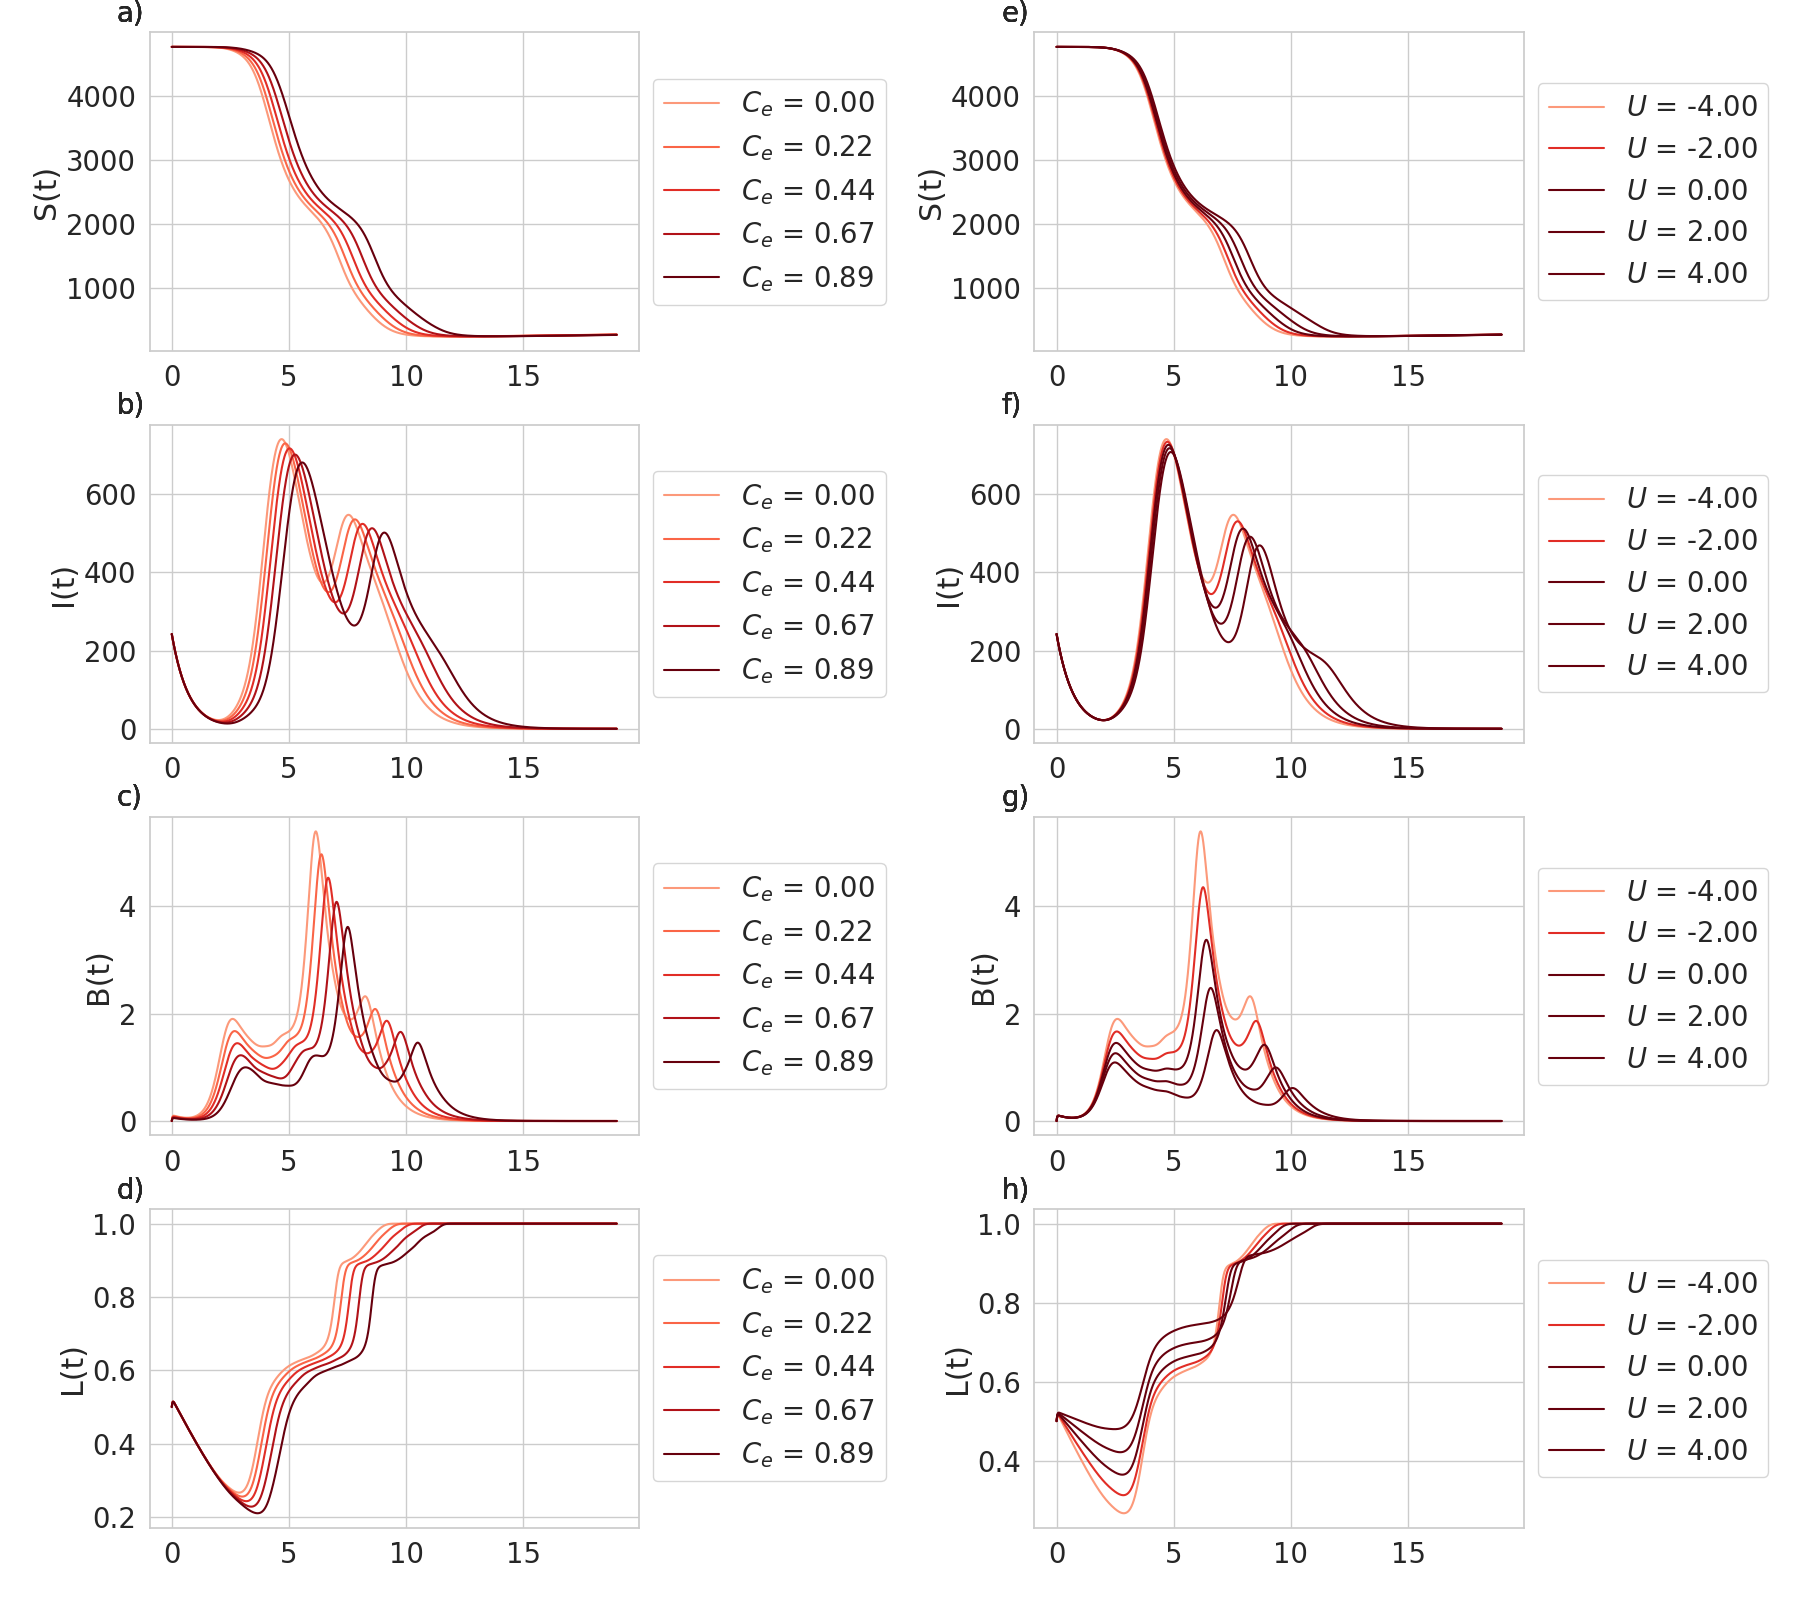
\includegraphics[width = \textwidth]{chapter_2/timeseries.png}
\caption{\textbf{Time series of model variables as a function of interventions, direct (raising $C_e$, panels a - d) and through social pressure (raising $U$, panels e - h)}. The former intervention, panels a-d, means an increase of social pressure on people who choose to transport firewood (i.e. increasing the $U$ value), and the latter refers to direct interception of firewood (i.e. increasing the $C_e$ value). Terms $L(t) = \frac{1}{N} \sum_{i = 1}^N S_i(t)$, $I(t) = \frac{1}{N} \sum_{i = 1}^N I_i(t)$, $B(t) = \frac{1}{N} \sum_{i = 1}^N B_i(t)$, $L(t) = \frac{1}{N} \sum_{i = 1}^N L_i(t)$ are the averages of the state variables over all patches. $S(t)$ has been omitted for brevity.}
\protect \label{ts}
\end{figure}

In Fig \ref{ct_v_ce} we show the total number of infested trees at time $t$, $T(t)$, with respect to combinations of $U$, the social cost to transport firewood, and the fraction of infested firewood intercepted, $C_e$. If the fraction of intercepted infested firewood, $C_e$, is greater than 80\%, we see a sharp reduction in the total infestation, $T$, even after 20 years (Fig \ref{ct_v_ce} c), but lower interception rates have little effect unless the social cost to transport $U$ is above the threshold seen in panel c) (Fig \ref{ct_v_ce}). Over a shorter time scale, increasing $C_e$ appears to be effective at all interception rates. 


The parameter $f$ controls how the proportion of strategists in a given patch $i$ ($L_i(t)$) responds to the population of infested trees ($I_i$) in that patch (eqn \ref{l_eqn}). Since social incentives (such as an intervention to human-mediated pest transport) tend to be less effective because they prevent firewood transport mostly in the areas that have already been colonized by pests (as suggested in Fig.\ref{ts}), we consider how the parameter $f$ affects the marginal returns on $U$ over time (Fig\ref{effectiveness_inset}). The shade of the blue region in Fig.\ref{effectiveness_inset} represents the degree to which increasing $U$ is beneficial, corresponding to a negative slope in the linear approximation of the change in $T$ with respect to $U$ (Fig \ref{effectiveness_inset} inset). Similarly, a red cell indicates non-negative slope and therefore a neutral or detrimental marginal effect. We begin to see the benefit of increasing $U$ after about 10 years, shown by the transition from lighter blue to dark blue as we move from the bottom of the image to the top (Fig \ref{effectiveness_inset}. This relationship is only affected slightly by altering the impact of local infestation on local strategy, $f$, where we begin to see slightly detrimental marginal returns after 10 years if $f < 0.04$.

Similarly, we have compared the marginal returns on increasing $U$ with respect to the intra-patch transmission rate $A$ and time $t$ (Fig \ref{A_v_time}). When $A$ is small ($A \leq 0.0009$, beneficial marginal returns on $U$ can be observed over the whole duration of the infestation. We further explore the impact of varying the rate of transmission of infested firewood between patches, $d$ (Fig \ref{A_v_d}). We find a roughly parabola-shaped region in the parameter plane of intra-patch and inter-patch transmission rates ($A$ and $d$ respectively), above which the marginal returns of increasing $U$ are zero or possibly detrimental to the size of the total infested population after 10-20 years. Larger intra-patch transmission rates enable the pest population to establish earlier in a given patch by propagules. We see good marginal return in parameter regimes where few transport strategists (high $L(t)$) would reduce the reproductive ratio of the infection below 1. For instance, at the point $(A,d) = (0.00126,0.103)$ , increasing $U$ is able to delay and eventually prevent a second wave, which decreases the total number of infected trees significantly (SI Fig 1). If the transmission rates $A,d$ are high enough that even with no transport strategists, we get a second wave of infection, the effect of increasing $U$ can be slightly detrimental (SI Fig 2). Panel f) of the aforementioned figures plots the number of patches where $I \geq 1$ over time, showing that the detrimental effect is largely due to the infection persisting longer in the network. 


\begin{figure}[!h]
 \centering
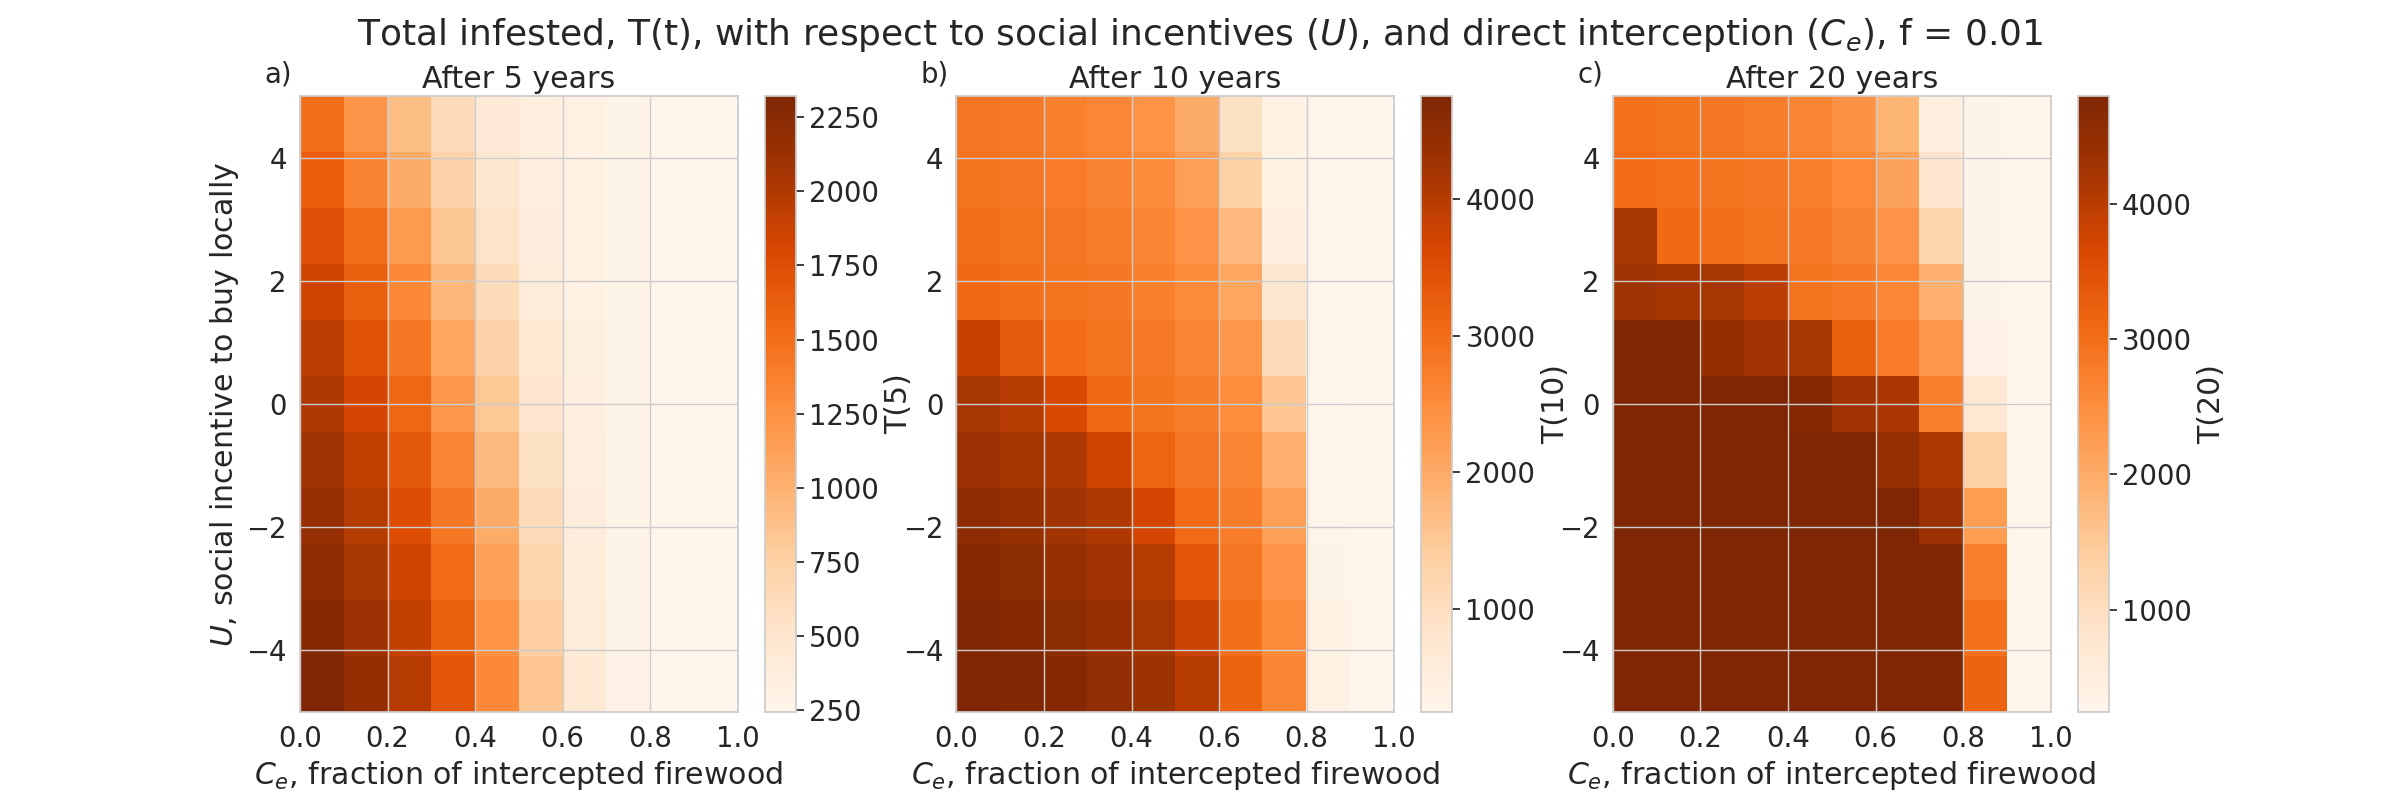
\includegraphics[width  =\textwidth]{chapter_2/ct_v_ce_plane.png}
\caption{\textbf{Total infestation per node over 5, 10 and 20 years.} Neither increasing $U$ nor $C_e$ are effective at long time scales.}
\protect \label{ct_v_ce}
\end{figure}



\begin{figure}[!h]
    \centering
    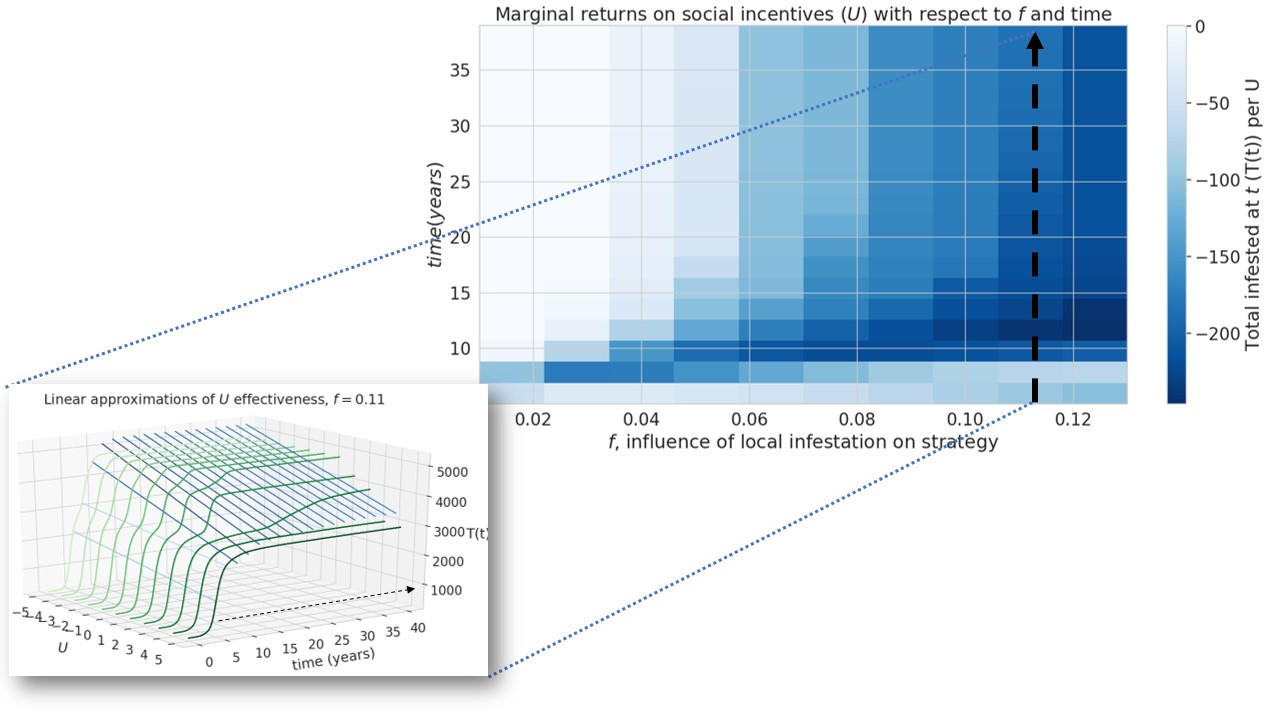
\includegraphics[width = \textwidth]{chapter_2/p1.jpg}
    \caption{\textbf{Efficacy of social incentives on infestation after time $T$. Inset graph shows an example of cross-section along the line $f = 0.11$} The influence of infestation on transport strategy, $f$, can hinder the intervention by public outreach, in the long-term (after approximately 20 years). The inset figure illustrates how one column in the heat map, shown by the dotted line, is constructed from the slopes of linear approximations of $T(t)$ over $U\in [-5,5]$. The blueness of the lines going left to right is a function of their slope, corresponding to the color of the cells in the heatmap.}
    \label{effectiveness_inset}
\end{figure}

\begin{figure}[!h]
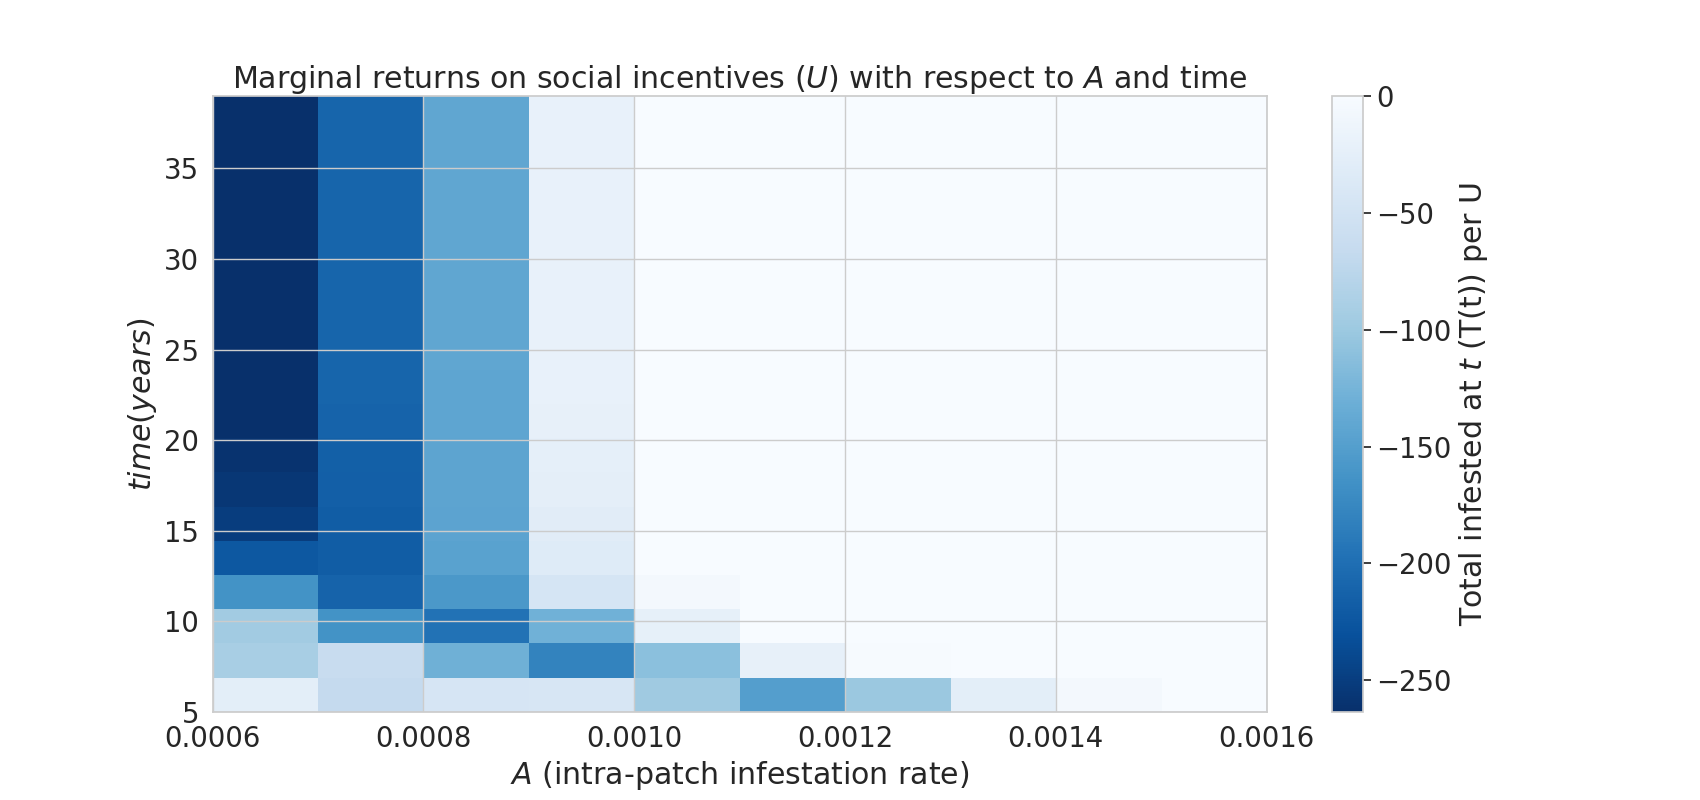
\includegraphics[width=\textwidth]{chapter_2/A_v_time.png}
\caption{\textbf{Efficacy of social incentives on infestation after time period $T$ with respect to $A$, the intra-patch infestation parameter.} This intervention becomes ineffective over time if $A$ is sufficiently large.}
\protect \label{A_v_time}
\end{figure}




\begin{figure}[!h]
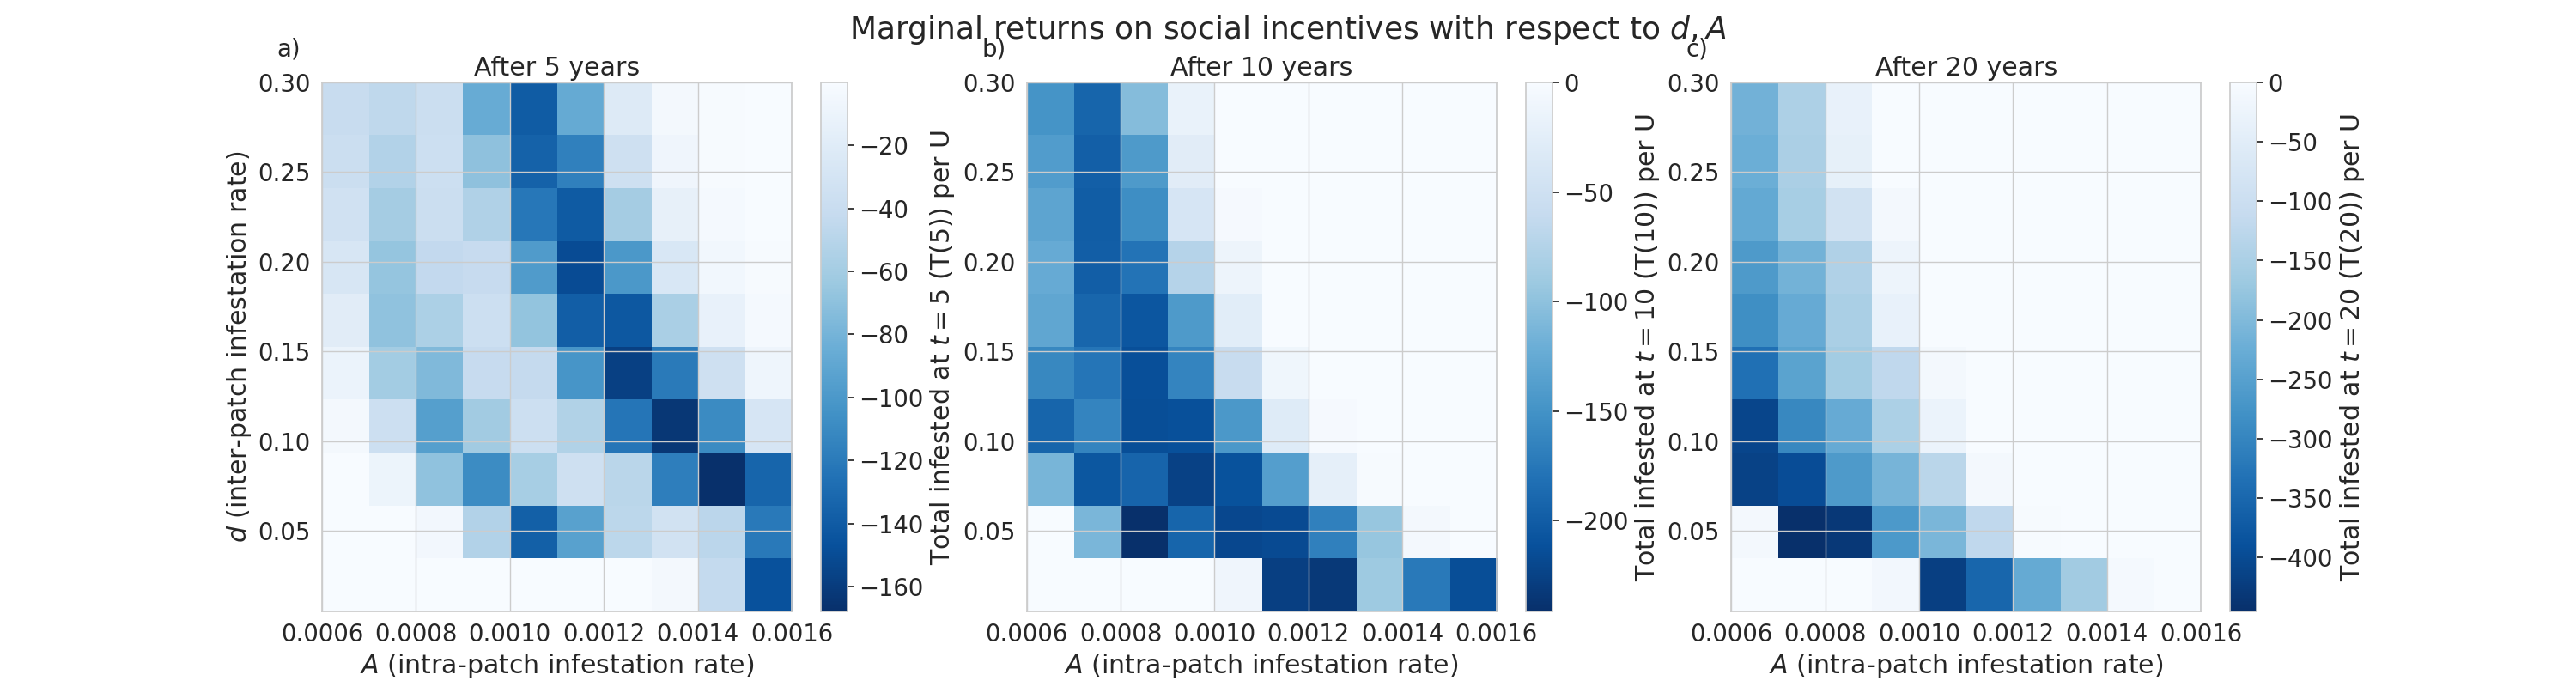
\includegraphics[width = \textwidth]{chapter_2/A_v_ct_v_d_marginal_gain.png}
\caption{\textbf{Efficacy of social incentives on infestation after time $T$ intra-patch spreading rate $A$, affects infestation outcomes.} The social incentive to not transport firewood, $U$, is more effective with lower pest spread rates.}
\protect \label{A_v_d}
\end{figure}


We also explored the effectiveness of patch quarantine by replacing model equations (\ref{i_eqn}) and (\ref{b_eqn}) with equations (\ref{i_eqn_modified_1})-(\ref{b_eqn_modified_2}). This replacement prevents individual patches (nodes in a set $V$) with the highest betweenness centrality (with respect to the weights $P_{ij}$) from interacting with their neighbours during the time of the quarantine $(t \in [t_0, t_0 + \Delta t])$. Imposing quarantine on these nodes is expected to have the greatest impact on pest transmission rate. If the quarantine is initiated one year after the pest is introduced into the system (that is, $t_0 = 1.0$) then we find a significant reduction in total infestation even if only 50 patches are quarantined ($|V| = 50$) assuming they are quarantined for more than a year, shown in Fig \ref{patch_quarantine_figure_t_0}. However, in our model, we find that quarantines need to be longer than approximately three years, and involve more than 150 nodes to still be effective in reducing the total infested population after 20 years $T(20)$. An interesting result in our quarantine plots is that we see a slightly larger range of effective parameter values if the quarantine begins after two years, $t_0 = 2.0$ (Fig \ref{patch_quarantine_figure_t_1}), rather than one, $t_0 = 1.0$. This effect is probably due to the delay in infestation after the model is initialized, which can be seen by the local minimum in the infestation timeseries (Fig \ref{ts}b,f). 


\begin{figure}[!h]
    \centering
    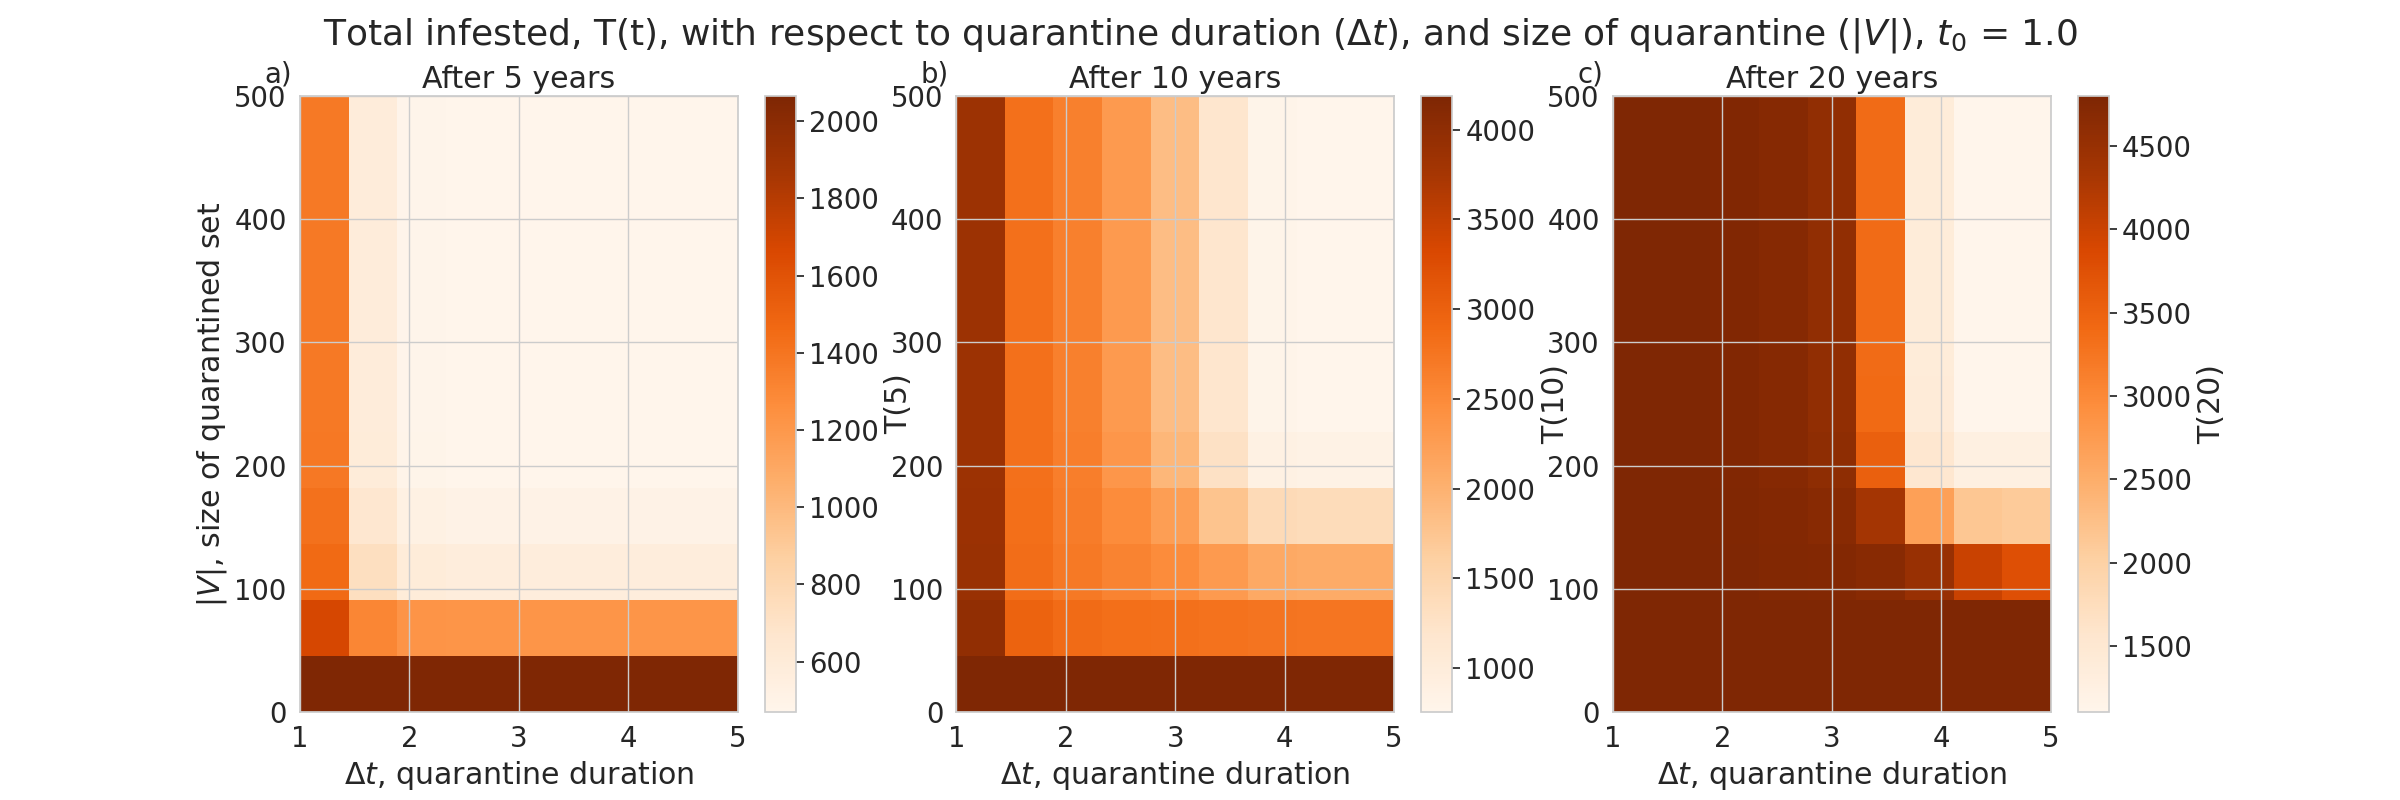
\includegraphics[width =\textwidth]{chapter_2/node_quarantine_plot_1.0.png}
    \caption{\textbf{Average total infested trees ($T(t)$) after 5, 10 and 15 years (panels a),b), and c) respectively), assuming the quarantine begins one year after the pest is introduced.} Total infestation plotted with respect to the number of nodes quarantined ($|V|$) and the length of the quarantine ($\Delta t$). The quarantine is effective over 5 years with only 50 patches, provided they are closed for over a year.}
    \label{patch_quarantine_figure_t_0}
\end{figure}

\begin{figure}[!h]
    \centering
    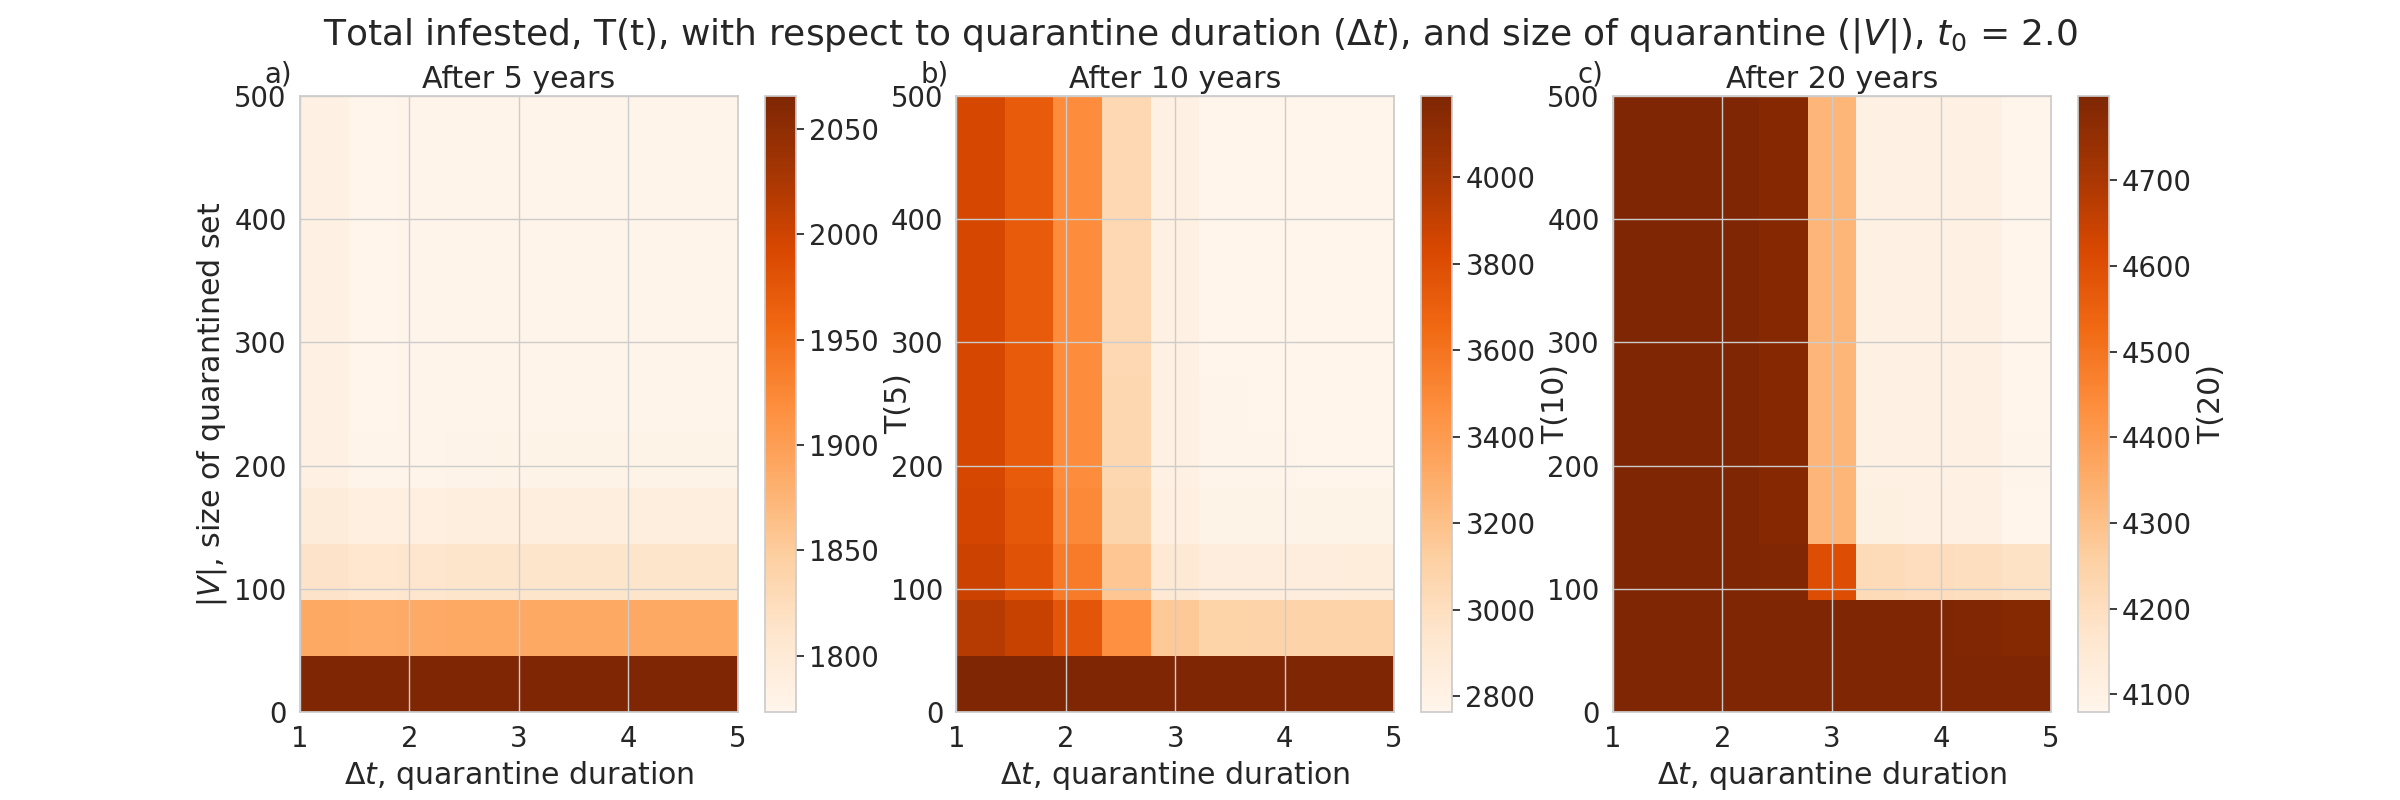
\includegraphics[width =\textwidth]{chapter_2/node_quarantine_plot_2.0.png}
    \caption{\textbf{Average total infested trees ($T(t)$) after 5, 10 and 15 years (panels a),b), and c) respectively), assuming the quarantine begins two years after the pest is introduced.} Total infestation plotted with respect to the number of nodes quarantined ($|V|$) and the length of the quarantine ($\Delta t$).}
    \label{patch_quarantine_figure_t_1}
\end{figure}


\section{Conclusion}

We presented a model coupling human social behaviour regarding transport of infested firewood through recreational travel with a model of the spread of an invasive forest pest. Our main focus was to compare, in relative terms, common measures for slowing the spread of invasive species with firewood transport, such as public outreach campaigns aimed to raise awareness about the problem, and enforcement measures, including inspections at checkpoints to control the movement of firewood, and location-specific quarantine. The model is parameterized with campground reservation data for provincial parks and campgrounds in the provinces of Ontario, Manitoba and Quebec, Canada and incorporated spatial information on the topology and geographical configuration of the camper travel network.

Under the assumptions of our model and a particular camper travel network configuration used in our model, checkpoints to control the movement of untreated firewood are unlikely to be effective at slowing the spread of invasive forest pests with firewood transport given typical moderate levels of funding and long delays in the response measures. We find the rate of interception to halve the total infested tree population after 5 years is about 30\% (Fig \ref{ct_v_ce}), which is unlikely to be achieved in practice given typical limited budgets and personnel constraints in present-day firewood control programs. Given that our model uses somewhat simplified assumptions and does not account for fine-scale logistical constraints (which inspectors may face in various spatial locations) the actual rate of interception is likely to be lower in practical conditions. While a previous study \cite{barlow2014modelling} that used a similar model has demonstrated that social incentives may improve outcomes in a two-patch model under equilibrium conditions, we have found that in our complex landscape network, the outcomes of infestation and invasion control measures are highly dependent on the time scale and the characteristics of the invaders, such as the inter-patch and intra-patch infestation rate. Social incentives (which aim to decrease the transport of firewood, $U$), are generally able to reduce the infestation rate in the short term but its effectiveness is highly dependent on the ability of the pest to spread and infest other locations (Fig \ref{A_v_d},\ref{A_v_time}) under the conditions we have explored. Humans in our model tend to reduce their transport of firewood between patches in already infested areas, which causes the pest to persist longer in the network (Fig \ref{ts}). Our results show that there could exist a threshold in the pest transmission rate $A$ and the proportion of the infested wood which is turned into firewood, $d$ (Fig \ref{A_v_d}). Below this threshold, it would not be beneficial to increase social outreach (i.e., increase $U$). This insight could be helpful in determining the spatial allocation of firewood movement control efforts for a particular pest species. We have also found that the location-specific quarantines that aim to restrict the movement of firewood to/from a particular location, might only be effective at slowing the invasion spread if a sufficiently large number (at least 140 in our case) of highly connected locations is quarantined, and the quarantine is established at early stages of infestation (Fig\ref{patch_quarantine_figure_t_0},\ref{patch_quarantine_figure_t_1}).

Given the typical cost limitations and logistics constraints faced by today’s firewood control programs, and the assumptions made in our modeling framework, it is unlikely that local quarantine measures could significantly slow the spread of invasive pests through firewood unless drastic control and quarantine measures are undertaken. Public outreach campaigns, while helping increasing awareness of problem, cannot reliably slow the spread of pests within the parameter values tested, when the invasion spreads through a network based on camper travel data in Manitoba, Ontario and Quebec. Within our model, public outreach could be more effective for slow-spreading pests when the organism is able to kill host trees quickly but does not have significant spread capacity (that is, the inter-patch and intra-patch infestation rates are sufficiently small). Direct intervention, such as checkpoint inspections for illegally transported firewood, is also not an option, because meaningful outcomes can only be achieved if significant fractions of firewood transports can be intercepted. We find that patch quarantine is effective at slowing, or even stopping, the spread of an invasive forest pest when a large number of highly-connected patches are quarantined, for a long enough period. Our results in general terms agree with a present-day situation when numerous outreach and local quarantine measures had limited impact on illegal transport of firewood by campers and failed to slow the spread of wood-boring pests transported with untreated firewood. Our results also indicate that the enforcement campaigns aimed to intercept illegal movement of untreated firewood can only be effective if implemented at very large spatial scales in timely fashion (which, in turn, would require massive amounts of funding and personnel support).

There are some shortcomings to our model that could be addressed in future work. The interventions we study do not have spatial or time specifications for individual locations in the camper travel network.  Deciding where and when, to deploy the outreach and enforcement measures in a particular location would be a major enhancement of the model. Second, our model depicted a general problem of an invasive pest spreading with untreated firewood moved by recreational travelers. To adapt the problem to a particular pest species, a more specialized spread model will be required. We simplified the model by assuming that each infested patch provides similar propagule pressure to recreational travellers leaving the infested site. This assumption was made because no data about the actual proportions of infested wood carried by recreational travellers leaving the infested sites were available. Also, our analysis did not offer much insight at the level of individual spatial locations in a camper travel network. A simpler mechanistic model that applies unique pest control decisions at individual spatial locations could potentially address that aspect. Another possible way to simplify the model would be to remove the tree growth dynamics —since it operates on a longer time scale than the infestation spread— and so an invasion model without the forest growth component could be a reasonable approximation for short-term planning horizons. This will be the focus of future efforts. 

\section{Acknowledgements}
The authors would like to thank Dr. Hanno Seebens and an anonymous reviewer for their contributions. Their detailed and thorough suggestions have significantly improved the quality of our paper.

% \nolinenumbers
% \bibliography{ref}




\chapter{Prioritising COVID-19 vaccination in changing social and epidemiological landscapes: a mathematical modelling study}
\label{ch3}
\begin{abstract}
  During the COVID-19 pandemic, authorities must decide which groups to prioritise for vaccination in a shifting social–epidemiological landscape in which the success of large-scale non-pharmaceutical interventions requires broad social acceptance. We aimed to compare projected COVID-19 mortality under four different strategies for the prioritisation of SARS-CoV-2 vaccines. We developed a coupled social–epidemiological model of SARS-CoV-2 transmission in which social and epidemiological dynamics interact with one another. We modelled how population adherence to non-pharmaceutical interventions responds to case incidence. In the model, schools and workplaces are also closed and reopened on the basis of reported cases. The model was parameterised with data on COVID-19 cases and mortality, SARS-CoV-2 seroprevalence, population mobility, and demography from Ontario, Canada (population 14.5 million). Disease progression parameters came from the SARS-CoV-2 epidemiological literature. We assumed a vaccine with 75\% efficacy against disease and transmissibility. We compared vaccinating those aged 60 years and older first (oldest-first strategy), vaccinating those younger than 20 years first (youngest-first strategy), vaccinating uniformly by age (uniform strategy), and a novel contact-based strategy. The latter three strategies interrupt transmission, whereas the first targets a vulnerable group to reduce disease. Vaccination rates ranged from 0.5\% to 5\% of the population per week, beginning on either Jan 1 or Sept 1, 2021. Case notifications, non-pharmaceutical intervention adherence, and lockdown undergo successive waves that interact with the timing of the vaccine programme to determine the relative effectiveness of the four strategies. Transmission-interrupting strategies become relatively more effective with time as herd immunity builds. The model predicts that, in the absence of vaccination, 72000 deaths (95\% credible interval 40000–122000) would occur in Ontario from Jan 1, 2021, to March 14, 2025, and at a vaccination rate of 1.5\% of the population per week, the oldest-first strategy would reduce COVID-19 mortality by 90.8\% on average (followed by 89.5\% in the uniform, 88.9\% in the contact-based, and 88.2\% in the youngest-first strategies). 60000 deaths (31000–108000) would occur from Sept 1, 2021, to March 14, 2025, in the absence of vaccination, and the contact-based strategy would reduce COVID-19 mortality by 92.6\% on average (followed by 92.1\% in the uniform, 91.0\% in the oldest-first, and 88.3\% in the youngest-first strategies) at a vaccination rate of 1.5\% of the population per week.Interpretation The most effective vaccination strategy for reducing mortality due to COVID-19 depends on the time course of the pandemic in the population. For later vaccination start dates, use of SARS-CoV-2 vaccines to interrupt transmission might prevent more deaths than prioritising vulnerable age groups.

\end{abstract}


\section{Introduction}


The COVID-19 pandemic has imposed a massive global health burden as waves of infection to move through populations around the world \cite{miller2020disease}.  Both empirical analyses and mathematical models conclude that non-pharmaceutical interventionsn (NPIs) are effective in reducing COVID-19 case incidence \cite{anderson2020estimating,peak2020individual,tuite2020mathematical}.  However, pharmaceutical interventions are highly desirable given the socio-economic costs of lockdown and physical distancing.  Hence, dozens of vaccines are  in development \cite{lurie2020developing}, and  model-based analyses are exploring the question of which groups should get the COVID-19 vaccine first \cite{bubar2020model,hoyt2020vaccine}.  


When vaccines become available, we will face a very different epidemiological landscape from the early pandemic. Many populations will already have experienced one or more waves of COVID-19.  As a result of natural immunity, the effective reproduction number $R_{eff}$ (the average number of secondary infections produced per infected person) will be reduced from its original value of approximately $R_0 = 2.2$ in the absence of pre-existing immunity \cite{hilton2020estimation}. Epidemiological theory tells us that as $R$ (or $R_0$) decline toward 1, the indirect benefits of transmission-blocking vaccines become stronger.  For instance, if $R_{eff} \approx 1.5$, such as for seasonal influenza, only an estimated $33 \%$ percent of the population needs immunity for transmission to die out in a homogeneously mixing population  \cite{anderson1992infectious,dushoff2007vaccinating}.  This effect was evidenced by the strong suppression of influenza incidence in Australia in Spring 2020 due to NPIs targeted against COVID-19 \cite{aussie2020}. 

This effect has stimulated a literature comparing the vaccination of groups that are responsible for most transmission to vaccination of groups that are vulnerable to serious complications from the infection. Natural immunity to SARS-CoV-2 will likely continue to rise in many populations on account of further infection waves. Given these likely changes to the epidemiological landscape before the vaccine becomes available, we suggest this question is worthy of investigation in the context of COVID-19. 


The social landscape will also look very different when vaccines become available and this aspect is crucial to understanding the pandemic. Scalable non-pharmaceutical interventions (NPIs) like physical distancing, hand-washing and masks are often one of the few available interventions when a novel pathogen emerges. Flattening the COVID-19 epidemic curve was possible due to a sufficient response by populations willing to adhere to public health recommendations. Therefore, pandemic waves are not simply imposed on populations -- they are a creation of the population response to the pathogen. They exemplify coupled socio-epidemiological systems exhibiting two-way feedback between disease dynamics and behavioural dynamics interact with one another \cite{pedro2020conditions}.

Approaches to modelling coupled social-epidemiological dynamics vary\cite{reluga2010game,salathe2008effect,funk2009spread,verelst2016behavioural,funk2010modelling}.  Some models have used evolutionary game theory to model this two-way feedback in a variety of coupled human-environment systems \cite{pedro2020conditions,bauch2005imitation,innes2013impact,bury2019charting,amaral2020epidemiological,zhao2020imitation,alam2020based}.  Evolutionary game theory captures how individuals learn social behaviours from others while weighing risks and benefits of different choices. In this framework, individuals who do not adopt NPIs can “free-ride” on the benefits of reduced transmission generated by individuals who do adopt NPIs \cite{reluga2010game}. 

Here, our objective is to compare projected COVID-19 mortality under four strategies for the prioritisation of COVID-19 vaccines: older individuals first, children first, uniform allocation, and a novel strategy based on the contact structure of the population. We use an age-structured model of SARS-CoV-2 transmission, including evolutionary game theory to model population adherence to NPIs and changes to mobility patterns.  We use scenario and sensitivity analysis to identify how strategy effectiveness responds to possible changes in the social-epidemiological landscape that may occur before and after vaccines become available.  

\section{Model Overview}

\subsection{Structure and parameterisation}

We developed an age-structured SEPAIR model (Susceptible, Exposed, Presymptomatic, Asymptomatic, Symptomatic, Removed) with ages in 5-year increments. Upon infection, individuals enter a latent period where they are infected but not yet infectious (“Exposed”).  After the latent period, individuals become presymptomatically infectious, and then either symptomatically or asymptomatically infectious, before finally entering the Removed compartment when their infectiousness ends. We did not model testing or contact tracing explicitly, although we assume infected individuals are ascertained at some rate. Transmission occurs through an age-specific contact matrix, susceptibility to infection is age-specific, and we include seasonality due to changes in the contact patterns throughout the year.  To infer model parameters, we fitted the model to Ontario COVID-19 case notifications stratified by age and time, Ontario seroprevalence data, and Ontario mobility data.  Use of seroprevalence data ensured that our estimates of transmission were not biased by case under-reporting. Remaining model parameter values were fixed using Ontario demographic and mortality data, and literature on COVID-19 serial interval and incubation periods.

Both schools and workplaces are closed when the number of ascertained active cases surpasses 50\%, 100\%, 150\%, 200\%, or 250\% of the peak ascertained active cases that occurred during the first wave (the “shutdown threshold”, T), and are re-opened again when cases fall below that threshold. Individuals interact with other individuals at a specified rate and switch between adherence and non-adherence to NPIs, including mobility restrictions, by comparing the cost of practicing NPIs against the cost of not practicing NPIs and thereby being subject to an increased risk of infection according to the prevalence of ascertained cases.  Both school and workplace closure and population level of adherence to NPIs reduce transmission according to a specified efficacy. 



\subsection{Model Equations}
 
Transmission dynamics are given by an SEPAIR model, modified to take population adherence to NPIs and school/workplace closure into account, and divided into age classes $i \in [1,16]$, where each age class contains a 5 year cohort, except for the oldest age group which comprises the ages $75$ and over. The model equations are:
\textcolor{black}{\begin{eqnarray}
\frac{dS^1_i}{dt} &= & - r \rho_i \left[1 + s \sin\left(\frac{2 \pi}{365} (t - \phi) - \frac{\pi}{2}\right)\right] S^1_i \sum_{j=1}^{16} C_{ij}(t) \left(\frac{I_{s_j} + I_{a_j} + P_j}{N_j}\right) - \tau S^1_i  \label{S1eqn} \\
\frac{dS^2_i}{dt} &= & - r \rho_i \left[1 + s\sin\left(\frac{2 \pi}{365} (t - \phi) - \frac{\pi}{2}\right)\right] S^2_i \sum_{j=1}^{16} C_{ij}(t) \left(\frac{I_{s_j} + I_{a_j}+ P_j}{N_j}\right)  - \tau S^2_i  \label{S2eqn} \\
\frac{dE_i}{dt} &= &  r_i \left[1 + s \sin\left(\frac{2 \pi}{365} (t - \phi) - \frac{\pi}{2}\right)\right]  (S^1_i + S^2_i) \sum_{j=1}^{16} C_{ij}(t) \left(\frac{I_{s_j} + I_{a_j}+ P_j}{N_j}\right) - \sigma_0 E_i + \tau (S^1_i + S^2_i)\label{Eeqn} \\
\frac{dP_i}{dt} &= & \sigma_0 E_i - \sigma_1 P_i \label{Peqn} \\
\frac{dI_{a_i}}{dt} &= & \eta \sigma_1 E_i - \gamma_a I_{a_i}\label{Ieqn} \\
\frac{dI_{s_i}}{dt} &= & (1 - \eta) \sigma_1 E_i - \gamma_s I_{s_i} \label{Ieqn} \\
\frac{dR_i}{dt} &= & \gamma_a I_{a_i} + \gamma_s I_{s_i}  \label{Reqn} \\
\frac{dD_i}{dt} &= & \Omega(D(t)) \label{Deqn} 
\end{eqnarray}}

\noindent Parameter values are defined in Table \ref{tab:params}. The vaccination dynamics are an impulsive process applied each day, described below. $S^{1}_i$ is the number of unvaccinated susceptible individuals in age group $i$, and $S^{2}_i$ is the number of susceptible individuals in age group $i$ who have received a standard two dose course of vaccination but were not immunized. $E_i(t)$ is the number of exposed but not yet infectious individuals in age group $i$ (\textcolor{black}{i.e., individuals in the latent period}). $I_{a_i}(t)$ is the number of asymptomatic infectious individuals in age group $i$ and $I_{s_i}(t)$ is the number of symptomatic infectious individuals in age group $i$. $R_i(t)$ is the number of Removed (recovered, vaccinated, and deceased) individuals in compartment $i$.

The variable $D(t) \in [0,1]$ in the model equation $dD(t)/dt = \Omega(D(t))$ represents the public health authority's reaction to the prevalence of ascertained cases and it evolves according to: 
\begin{eqnarray}
  \Omega(D(t)) =  \left\{
\begin{array}{ll}
    k_1 (1 - D(t)) &  \sum_{i=1}^{16}\alpha_i(I_{a_i} + I_{s_i}) > T\\
    - k_2 D(t) & \sum_{i=1}^{16}\alpha_i(I_{a_i} + I_{s_i}) \leq T
\end{array} 
\right. 
\end{eqnarray}
This represents closure being triggered when ascertained cases exceed a threshold $T$, and being lifted when cases drop below that threshold again. 

The proportion $x$ of individuals who practice NPIs such as mask wearing, handwashing, and physical distancing, starts off at $x(0)=0.01$ and evolves as: 
\begin{eqnarray}
\frac{dx}{dt} &= &\kappa x (1-x) \left(\frac{\sum_{i=1}^{16}\alpha_i(I_{a_i} + I_{s_i})}{\sum_{i=1}^{16} N_i} - c x\right) + p_{ul}(1-2 x) 
\label{xeqn_new}
\end{eqnarray}
where $\kappa$ is the social learning rate, $c$ is the incentive to not practice NPIs, and $\alpha_i$ is the fraction of total cases ($I_a + I_s$) that are reported, also known as the ascertainment rate.  The $p_{ul}$ term is a phenomenological term that represents the effects of social heterogeneity and influence from external populations that prevents the system from remaining arbitrarily close to $x=0$ or $x=1$ for unrealistic periods of time.  These equations describe a population where individual sample other individuals at some time rate and switch between adherence and non-adherence to NPIs with a probability proportional to the expected gain in utility $\sum_{i=1}^{16}\alpha_i(I_{a_i} + I_{s_i}) - c x$. We refer the reader to existing literature for details on the derivation of this equation \cite{bauch2005imitation,innes2013impact,thampi2018socio,bauch2012evolutionary,oraby2014influence}. 

$C_{ij}(t,x)$ is the average number of contacts per day and consists of contacts at workplaces, schools, households, and other locations, which vary depending on government shutdown policies as well as indivdual adherence to NPIs like physical distancing and mask use: 
\begin{eqnarray}
C_{ij}(t,x) &= & C^W_{ij}(t) + C^S_{ij}(t) + (1 - \epsilon_P x ) (\overline{C}^O_{ij} + \overline{C}^H_{ij} )
\end{eqnarray}
The contacts in each of the aforementioned places can vary as follows. At workplaces, which can be closed by public health authorities: 
\begin{eqnarray}
C^W_{ij}(t) =  \left\{
\begin{array}{ll}
      (1 - \epsilon_W) \overline{C}^W_{ij} & t - t_{delay} >t_{close}, t  - t_{delay}< t^w_{open} \\ 
      \overline{C}^W_{ij} &  t - t_{delay}<t^w_{close} \\
       
       (1 - D(t)(1 - \epsilon_W)) \overline{C}^W_{ij} & t - t_{delay}> t^w_{open}
\end{array} 
\label{cw_eqn}
\right. 
\end{eqnarray}
where $\overline{C}^W_{ij}$ is the normal (non-pandemic) number of contact-hours per day between individuals of age $i$ and $j$ at the workplace \cite{zagheni2008using}; $\overline{C}^W_{ij} (1 - D(t)\epsilon_P)$ is the reduced rate under workplace closure efficacy $0 < \epsilon_W< 1$ and closure level $D(t)$; and $t_{delay}$ represents the delay between the decision to adopt NPIs and their impact on transmission \cite{li2020temporal}. Lower than perfect efficacy may stem either from occasional use of workplace for critical needs or non-authorized access, workplaces that remain open because they provide essential services, etc. $t^W_{close}$ and $t^W_{open}$ are the times of closing and re-opening workplaces, respectively. Similarly, for schools we have: 
\begin{eqnarray}
  C^S_{ij}(t) =  \left\{
\begin{array}{ll}
      0 & t - t_{delay}>t^s_{close}, t - t_{delay} < t^s_{open} \\ 
      \overline{C}^S_{ij} &  t - t_{delay}<t^s_{close} \\
       
      (1 - D(t)) \overline{C}^S_{ij} & t - t_{delay} > t^s_{open}
\end{array} 
\right. 
\label{cs_eqn}
\end{eqnarray}
All other places of exposure are governed by social processes with imperfect ability of public health authorities to enforce mandates, and hence are governed by voluntary population adherence to NPIs such as mask use and physical distancing as per the $\epsilon_P x(t)$ term in the equation, where $\epsilon_P$ is efficacy of individual adoption of NPIs.  In principle, contact hours spent at home should increase as workplaces and schools are closed, but we assume that infection probabilities will saturate rapidly with contact hours in the home. Each of the conditional functions in equations (\ref{cw_eqn},\ref{cs_eqn}), are represented in the model as a smoothed step function with a steep slope, and we restrict them between $0$ and $1$ if the smoothing process would cause the closure level $D(t)$ to exceed 1.0.   Finally, our interventions (school and workplace shutdown) do not distinguish between preventing contacts in “home” versus “other” locations. \textcolor{black}{We assume the same efficacy of NPIs in home as in ''other" locations.  On one hand, individuals are less likely to use NPIs at home.  On the other hand, contacts at home are repeated and thus there is a saturating effect that can somewhat reduce the infection risk, compared to the diversity of contacts experienced in the general community.  Additionally, our case notifications are not broken down by the location of infection and thus we have limited ability to parameterize two difference NPI efficacy in home and ''other" locations.  As a result, we assume the same efficacy in both settings.}

\subsection{Vaccination process}
 \textcolor{black}{Each day, the total number of individuals vaccinated is equal to $\sum_{i = 1}^{16} \phi \frac{S_i(t)}{N_i}$, and the number of individuals immunized against transmission of the virus is $\sum_{i = 1}^{16} v_{T_i} \frac{S_i(t)}{N_i - V_i}$ on account of imperfect vaccination. The factor $\frac{S_i(t)}{N_i - V_i}$ represents vaccination of each person with equal probability, so the probability of vaccinating a susceptible person decreases with the fraction of susceptible individuals out of the non-vaccinated people.} If there are less than $\phi_i$ individuals in group $S^1_i$, then the remainder of the vaccine is spread evenly among the remaining non-vaccinated groups. Individuals who are vaccinated but not immunized due to imperfect efficacy are moved to the corresponding $S^2_i$. We assume that a course of vaccination will not be administered to a person more than twice.

The fraction of people who are vaccinated against disease but not against transmissibility is $v_{D_i} - v_{T_i}$. We assume this fraction of people is still able to transmit the disease normally, and therefore we account for them by reducing the mortality rate (see Supp. ~Mortality computation). 


\subsection{Differences between parameters in the first and second wave}


 \textcolor{black}{To account for the differences in social response, to the first and second waves of the infection, we assume that the social dynamics variables $\kappa$ (the social learning rate), and $c$ (the incentive not to distance). We assume that these variables are functions of time, which transition between two values at a time $t_{switch} = 160$ days after the beginning of the pandemic.
\begin{align}
    \kappa &= \kappa(t) = \kappa_2 \left(\frac{\tanh\left(k_s(t - t_{switch})\right) + 1}{2}\right) +  \kappa_1 \left(1 - \frac{\tanh\left(k_s(t - t_{switch})\right) + 1}{2}\right)\\
    c &= c(t) = c_2 \left(\frac{\tanh\left(k_s(t - t_{switch})\right) + 1}{2}\right) + c_1 \left(1 - \frac{\tanh\left(k_s(t - t_{switch})\right) + 1}{2}\right)
\end{align}
We chose the rate of switch, $k_s= 0.05$ to take 2 - 4 weeks.}

\subsection{Case under-ascertainment} 
 \textcolor{black}{
Case under-ascertainment of the $ith$ age group is represented by the following function:
\begin{eqnarray}
\alpha_i(t) = \left\{
  \begin{array}{ll}
          \alpha_{i,2} & t >t_{switch}\\ 
          \alpha_{i,1}\left(\frac{t_{switch} - t}{t_{switch}}\right) & t \leq t_{switch}\\
    \end{array} 
 \right.
\end{eqnarray}
where where $\alpha_{1,1}, \alpha_{2,1}, \alpha_{3,1}$ corresponds to the ascertainment in the age groups $(0,20),(20,60),> 60$ at $t = 0$, respectively. We assume that the ascertainment rises to a value of $\alpha_{1,2}, \alpha_{2,2}, \alpha_{3,2}$ in the age groups $(0,20),(20,60),> 60$ respectively, at $t = t_{switch}$, denoting the increase in ascertainment throughout the first wave and into the second wave. We multiply the infections in each age group $i$ at time $t$ by the corresponding $\alpha_i(t)$ after the simulation is finished.}

\subsection{Baseline transmission rate} 

We can compute $r$ as a function of the next-generation matrix, $M = - \Theta \Sigma ^{-1}$  \cite{diekmann2010construction}, where $\Theta$ and $\Sigma$ are defined as in equations \ref{Teqn},\ref{Sigmaeqn}, and so $M$ is a function of \textcolor{black}{ $R_0, \sigma_0,\sigma_1, \gamma_a, \gamma_s, \eta, C(t),$} and $N$. These matrices come from the rate at which infected individuals enter and leave the  infection compartments when the system is linearized about the $I_a = 0, I_s = 0, P = 0$ equilibrium. The basic reproduction ratio, $R_0$, of the infection is the spectral radius of $M$, written $\rho(M)$. We can pull $r$ out of this expression and write $r$ in terms of the other parameters: $r = \frac{R_0}{\rho(M)}$.
\footnotesize
\textcolor{black}{
\begin{equation}
    \Theta = 
\begin{bmatrix}
0 & \dots & 0  & \frac{r C_{1,1}(0)N_1}{N_1} & \dots &\frac{r C_{1,n}(0)N_1}{N_n} &  \frac{r C_{1,1}(0)N_1}{N_1} & \dots & \frac{r C_{1,n}(0)N_1}{N_n} &  \frac{r C_{1,1}(0)N_1}{N_1} & \dots & \frac{r C_{1,n}(0)N_1}{N_n}  \\
\vdots & \ddots  & \vdots & \vdots & \vdots & \ddots  & \vdots & \ddots & \vdots  & \vdots & \ddots & \vdots \\
0 & \dots & 0 & \frac{r C_{1,n}(0)N_n}{N_1} & \dots & \frac{r C_{n,n}(0)N_n}{N_n}  & \frac{ r C_{1,n}(0)N_n}{N_1} & \dots & \frac{r C_{n,n}(0)N_n}{N_n} & \frac{ r C_{1,n}(0)N_n}{N_1} & \dots & \frac{r C_{n,n}(0)N_n}{N_n} \\ 
0 & \dots & 0  & 0 & \dots & 0  & 0 & \dots & 0 & 0 & \dots & 0  \\
\vdots & \ddots & \vdots & \vdots &  \ddots & \vdots & \vdots & \ddots & \vdots & \vdots & \ddots & \vdots\\
0 & \dots & 0  & 0 & \dots &  0  & 0 & \dots & 0  & 0 & \dots & 0 \\ 
0 & \dots & 0  &  0 & \dots & 0  & 0 & \dots & 0  & 0 & \dots & 0 \\
\vdots & \ddots & \vdots & \vdots & \ddots & \vdots & \vdots & \ddots & \vdots  & \vdots & \ddots & \vdots\\
0 & \dots & 0  & 0 & \dots & 0  & 0 & \dots &  0 & 0 & \dots &  0 \\ 
0 & \dots & 0  &  0 & \dots & 0  & 0 & \dots & 0  & 0 & \dots & 0 \\
\vdots & \ddots & \vdots & \vdots & \ddots & \vdots & \vdots & \ddots & \vdots  & \vdots & \ddots & \vdots\\
0 & \dots & 0  & 0 & \dots & 0  & 0 & \dots &  0 & 0 & \dots &  0 \\ 
\end{bmatrix}
\label{Teqn}
\end{equation}
\begin{equation}
    \Sigma = 
\begin{bmatrix}
-\sigma_0 & \dots & 0  &  0 &\dots & 0  & 0 & \dots & 0   & 0 & \dots & 0  \\
\vdots & -\sigma_0  & \vdots & \vdots &  \ddots & \vdots & \vdots &0 & \vdots & \vdots &0 & \vdots\\
0 & \dots &-\sigma_0  & 0 & \dots & 0.0 & 0 & \dots & 0 & 0 & \dots & 0  \\ 
0 & \dots & 0 & -\sigma_1 & \dots & 0  & 0 & \dots & 0  & 0 & \dots & 0  \\
\vdots & \ddots & \vdots &\vdots & -\sigma_1  & \vdots & \vdots & \ddots  & \vdots & \vdots & \ddots & \vdots\\
0 & \dots & 0  & 0 & \dots &-\sigma_1   & 0 & \dots & 0 & 0 & \dots & 0 \\ 
0 & \dots & 0  & \eta\sigma_1  & \dots & 0  & -\gamma_a & \dots & 0  & 0 & \dots & 0  \\
\vdots & \ddots & \vdots & \vdots & \eta\sigma_1  & \vdots & \vdots &  -\gamma_a & \vdots & \vdots & \ddots & \vdots\\
0 & \dots & 0  & 0 & \dots &  \eta\sigma_1 & 0 & \dots &  -\gamma_a  & 0 & \dots & 0  \\ 
0 & \dots & 0  &   (1 - \eta)\sigma_1 & \dots & 0  &  0 & \dots & 0  &  -\gamma_s & \dots & 0  \\
\vdots & \ddots & \vdots & \vdots &  (1 - \eta)\sigma_1 & \vdots & \vdots & \ddots & \vdots & \vdots &  -\gamma_s & \vdots\\
0 & \dots & 0  &  0 & \dots & (1 - \eta)\sigma_1 & 0 & \dots & 0  & 0 & \dots &  -\gamma_s  \\ 
\end{bmatrix}
\label{Sigmaeqn}
\end{equation}}
\normalsize
\subsection{Disease progression parameters}

Transition rates for the duration of the asymptomatic infectious period and the proportion of symptomatic cases were obtained from COVID-19 epidemiological literature \cite{nishiura2020serial,lauer2020incubation,tindale2020transmission}.  We computed the mortality due to COVID-19 by applying the case fatality rate obtained from \cite{publichealthontario}, interpolated to 16 age groups.

\subsection{Initial conditions}

The point $t = 0$ was chosen to be the day at which the province of Ontario recorded more than 50 cases, March 10th 2020, to reduce the effects of stochasticity in the early case counts. Let the number of observed cases of COVID-19 in age group $i$ on March 10th 2020 be $\omega_i$. We use the age distribution of $\omega_i$ to determine the age distribution for $I_a(t) + I_s(t)$. The true number of cases that day is $\omega_i / \alpha_i$, where $\alpha_i$ is the ascertainment rate of cases in group $i$. Since we do not know the actual number of active cases, $I_{a_i}(t) + I_{s_i}(t)$ at $t = 0$, we assume the number of active cases is equal to the true number of incident cases multiplied by a constant $I_0$, which is also treated as a model variable to be fitted. Therefore, $I_{s_i}(0) = \eta I_0 \frac{\omega_i}{\alpha_i}$ and $I_{a_i}(0) = (1 - \eta) I_0 \frac{\omega_i}{\alpha_i}$.
\textcolor{black}{Similarly, we assumed that the numbers of presymptomatic and exposed cases at $t = 0$ are proportional to the number of ascertained incident cases in each age group, $\omega_i$. We fit the variables $P_0$ and $E_0$ so that $P(0) = P_0 \frac{\omega_i}{\alpha_i}$ and  $E(0) = E_0 \frac{\omega_i}{\alpha_i}$.} We assumed that\textcolor{black}{$S^1_i(0) = N_i  - (I_a(0) + I_s(0) + E(0) + P(0))$, so the total number of susceptible, unvaccinated individuals $\sum_{i = 1}^{16} S^1_i(0)$ is the population of the region (minus the number who begin in the infected compartments)}, and $S^2_i(0) = 0, E_i(0) = 0, R_i(0) = 0$ for all $i$. Lastly, we assumed that at $t = 0$, only 1\% of individuals are physical distancing, so $x(0) = 0.01$, and that $D(0) = 0$.

\subsection{Particle filtering}

We calibrated the model with data from Ontario, Canada. Since the workplace closure opening and closing rates, $k_1$ and $k_2$, are not coupled with the model, we fit a step function of the form $$f(t) = \epsilon_W \left( \tanh{k_1(t - t^W_{close})} - \tanh{k_2(t - t^W_{close})}\right)$$ to the \textrm{"workplaces\_percent\_change\_from\_baseline"} field of the Google mobility data \cite{googlemobility} for the province. We applied a particle filtering approach using intervals around selected parameters. Intervals used for sampling appear in Table \ref{tab:params}. \textcolor{black}{We fit the 7-day moving average of incident cases on each day across all age groups to the number of cases registered by Public Health Ontario on that day \cite{ontariocoviddata}, and also the total number of cases at the end of the fitting window for each age group. The decrease in contact-hours due to social distancing, $x(t)$, was fit to the decrease in the "Retail and Recreation" hours recorded by Google mobility \cite{googlemobility}}.  \textcolor{black}{The 1.1 $\%$ (0.8 $\%$, 1.3 $\%$)  of Ontario residents seropositive for COVID-19 in June 2021 was also used as a fitting criterion \cite{ontario_sero}.} The posterior distribution of the parameters was estimated with the approximate Bayesian computation scheme described in \cite{turner2012approximate}, with uniform priors and 200 particles, using the KissABC \cite{kissabc} library for the Julia language. The acceptance threshold was chosen to given acceptable variation and evaluation time.

%  Mobility data specific to school closure does not exist, so we assumed that outside of the normal school breaks (\textit{e.g.} summer holiday), schools exhibit similar temporal curves describing opening and closing as workplace do.  We used published COVID-19 case fatality rates to determine number of deaths by age group based on the predicted incident cases by age group. Posterior distribution of model fits to age-specific cumulative cases appear in Figure S2, and posterior model time series fits appear in Figure 1. 

\subsection{Vaccination refusal dynamics}
\textcolor{black}{In an extension to the model explored the dynamics of the model with the added complication of vaccine refusal. We introduce a variable $y(t)$ to represent that fraction of the population willing to be vaccinated for the virus, governed by imitation dynamics similar to the social distancing equation \ref{xeqn_new}. We add the following equation \ref{yeqn} to the rest of the model equations \cite{bauch2005imitation, bauch2012evolutionary}.
\begin{equation}
    \frac{d y}{dt} = \kappa_{vac} y(1 - y)\left(\frac{\sum_{i=1}^{16}\alpha_i(I_{a_i} + I_{s_i})}{\sum_{i=1}^{16} N_i} - c_{vac}\right)
    \label{yeqn}
\end{equation}
In the above equation, the vaccination decisions of the population are governed by a payoff function, where $c_vac$ is the payoff not to vaccinate, and the payoff to vaccinate is proportional to current the number of ascertained active infections. The initial condition for this variable, $y_0$ is assumed to be $0.67$ from \cite{MALIK2020100495}.}

\textcolor{black}{The population in age group $i$ that refuses to be vaccinated is $N_i (1 - y(t))$. We implement this mechanic in the model by assuming that the number of people vaccinated each day in age group $i$, $\psi_i$ is unchanged, except that the compartment $S_{v_i}^1$ is considered to be empty when $N_i (1 - y(t))$ people remain.}


\subsection{Model extension for vaccine efficacy against disease only}

We conducted the sensitivity analysis scenario distinguishing vaccine efficacy against disease only versus vaccine efficacy against both infectivity and disease by adjusting the case fatality rates according to vaccine coverage in the population and assumed efficacies. The adjustment factor is determined by the relative sizes of $S_1(t)$ and $S_2(t)$. Let $\xi_1 (S_1(t)) = \xi S_1(t)$ be the rate at which individuals in $S_1(t)$ are infected, and similarly $\xi_2 = \xi S_2(t)$ the rate at which individuals in $S_2(t)$ are infected. Let $S_3(t)$ be the number of people at $t$ who are immunized but still able to transmit the virus, and $\xi_3 = \xi S_3(t)$. We also assume that
\begin{equation}
   \frac{\xi_1(t)}{\xi_3(t)} = \frac{1 - v_{D_i}}{v_{D_i} - v_{T_i}}
   \label{vacassumption}
\end{equation}
which applies given that the timescale of infection in individuals is fast compared to the whole duration of the pandemic. The proportion of unvaccinated people who are infected at $t$ is $\frac{\xi_1(t)}{\xi_1(t) + \xi_2(t) + \xi_3(t)}$, and the fraction of vaccinated but not immunized people infected at $t$ is $\frac{\xi_2(t)}{\xi_1(t) + \xi_2(t) + \xi_3(t)}$. From equation \ref{vacassumption}, and the model equations, we can adjust the probability that a given person who is infected also dies at time $t$ as
\begin{equation}
    \textrm{Adjusted mortality at } t  \textrm{ for age group } i = \frac{S_{1_i}(t) + S_{2_i}(t)}{S_{1_i}(t) + S_{2_i}(t)\frac{1 - v_{T_i}}{1 - v_{D_i}}} \times \textrm{Cases at }t \times \textrm{measured CFR}
\end{equation}

\subsection{Vaccine scenarios} 

We considered two dates for the onset of vaccination: 1 March 2021 and 1 September 2021. These correspond to the end dates of a two-dose course of vaccination lasting two weeks. We assumed it was possible to vaccinate 0.5\%, 1.0\%, 1.5\%, 2.5\%, or 5.0\% of the population per week (the “vaccination rate”, ψ0).  Our baseline scenario assumed a vaccine with 75\% efficacy in all ages, against both infection and transmission.  

The “oldest first” strategy administers the vaccine to individuals 60 years of age or older, first.  After all individuals in this group are vaccinated, the vaccine is administered uniformly to other ages. The “youngest first” strategy is similar, except it administers the vaccine to individuals younger than 20 years of age first.  The “uniform” strategy administers vaccines to all age groups uniformly, from the very start. The “contact-based” strategy allocates vaccines according to the relative role played by different age groups in transmission. This tends to prioritise ages 15-19 primarily, 20-59 secondarily, and the least in older or younger ages.  The ``oldest first" strategy targets a vulnerable age group while the other three strategies are designed to interrupt transmission.


\clearpage 

\begin{table}[H]
\tiny
  \caption{Parameter definitions, values, particle filtering ranges, and sources.}
  \begin{tabular}{llll}
  Parameter & Meaning & Value [Range] & Source \\
  \midrule
  $N_i$         & Population in age group $i$  & $0-4$:  $790169$; $5-9$: $789190 $ & \cite{ontario_census}, interpolated\\
                &   & $10-14$: $790803$; $15-19$: $887072$ &  \\
                &   & $20-24$: $1003052$; $25-29$: $1015105$ &  \\
                &   & $30-34$: $1009090$; $35-39$:  $969949$ &  \\
                &   & $40-44$:  $926440$; $45-49$:  $938990$ &  \\
                &   & $50-54$:   $1027557$; $55-59$: $10416495$ &  \\
                &   & $60-64$:  $892016$; $65-69$:  $741824$ &  \\
                &   & $70-74$:  $557203$; $75+$:  $204431$ &  \\
  
  $\mu_i$       & COVID-19 case fatality rate in age group $i$  & $0-4$: $0.002$; $5-9$: $0.001$  & \cite{publichealthontario}, interpolated\\
                &   & $10-14$:   $0.0005$; $15-19$:  $0.0005$ &  \\
                &   & $20-24$:  $0.0010$; $25-29$:   $0.002$ &  \\
                &   & $30-34$:  $0.0031$; $35-39$:   $0.0048$ &  \\
                &   & $40-44$:   $0.0078$; $45-49$:   $0.0135$  \\
                &   & $50-54$:    $0.0253$; $55-59$:   $0.0455$ &  \\
                &   & $60-64$:   $0.0784$; $65-69$:  $0.1378$ &  \\
                &   & $70-74$:  $0.2623$; $75+$:   $0.5815$ &  \\
                
  $C_{ij}$    & contact rate between class $i$ and $j$    & see Methods & \cite{prem2020projecting} \\
  $R_0$ & basic reproduction rate of infection & calibrated, $[1.5,2.5]$ & \cite{hilton2020estimation,googlemobility, ontariocoviddata}  \\
  $r$         & probability of transmission per contact   & derived from next generation matrix & \cite{diekmann2010construction} \\
  $\sigma_0$    & inverse of latent period for exposed individuals                  & calibrated, $[0.3,2.0]$ & \cite{googlemobility, ontariocoviddata,nishiura2020serial,lauer2020incubation,tindale2020transmission} \\
  $\sigma_1$    & inverse of latent period for presymptomatic individuals & calibrated, $[0.3,2.0]$ & \cite{googlemobility, ontariocoviddata,nishiura2020serial,lauer2020incubation,tindale2020transmission} \\
  $\gamma_a$    & inverse of infectious period for asymptomatic individuals & $0.25$/day &  \cite{nishiura2020serial,lauer2020incubation,tindale2020transmission} \\
  $\gamma_s$    & inverse of infectious period for symptomatic individuals  & calibrated, $[0.0,0.05]$ & \cite{googlemobility, ontariocoviddata,nishiura2020serial,lauer2020incubation,tindale2020transmission} \\
  $\alpha_{1,1}$ & Ascertainment rate of class $i$ in the first wave (before $t_{switch}$) & calibrated, $[0.01,1.0]$ & see Methods\\
  $\alpha_{1,2}$ & Ascertainment rate of class $i$  in the first wave (before $t_{switch}$) & calibrated, $[0.01,1.0]$ & see Methods\\
  $\alpha_{1,3}$ & Ascertainment rate of class $i$ in the first wave (before $t_{switch}$) & calibrated, $[0.2,1.0]$ & see Methods\\
  $\alpha_{2,1}$ & Ascertainment rate of class $i$  in the second wave (after $t_{switch}$)& calibrated, $[0.01,1.0]$ & see Methods\\
  $\alpha_{2,2}$ & Ascertainment rate of class $i$ in the second wave (after $t_{switch}$) & calibrated, $[0.01,1.0]$ & see Methods\\
  $\alpha_{2,3}$ & Ascertainment rate of class $i$  in the second wave (after $t_{switch}$)& calibrated, $[0.2,1.0]$ & see Methods\\
  $\rho_1$ & Age-specific susceptibility modifier, ages 0-20 & calibrated, $[0.25,3.0]$  & see Methods\\
  $\rho_2$ & Age-specific susceptibility modifier, ages 20-60 & calibrated, $[0.25,3.0]$  & see Methods\\
  $\rho_3$ & Age-specific susceptibility modifier, ages 60+ & calibrated, $[0.25,3.0]$  & see Methods\\
  $\eta$ & fraction of symptomatic infections & $0.15$ & \cite{mizumoto2020estimating} \\
  $\epsilon_P$ & efficacy of physical distancing  & calibrated, $[0.3,0.9]$ & \cite{googlemobility, ontariocoviddata}  \\
  $\kappa$    & social learning rate   & calibrated, $[1000,16000]$ & \cite{googlemobility, ontariocoviddata} \\
  $ s $ & seasonality & calibrated, $[-0.3,0.3]$ & \cite{googlemobility, ontariocoviddata} \\
  $\phi$  & seasonality phase & $-30$ days & see Methods \\
  $ v_{T_i} $ & Vaccine efficacy against transmissibility and disease for individuals in group $i$  &  $75 \%$  & \cite{WHO_TPP} \\
  $ v_{D_i} $ & Vaccine efficacy against disease only for individuals in group $i$  &  $75 \%$  & \cite{WHO_TPP} \\
  $ I_0 $ & Initial ratio of active cases to incident cases & calibrated, $[1,10]$ & \cite{googlemobility, ontariocoviddata} \\
  $ P_0 $ & Initial ratio of presymptomatic cases to incident cases & calibrated, $[1,10]$ & \\
  $ E_0 $ & Initial ratio of exposed cases to incident cases & calibrated, $[1,10]$ & \\
  $\psi_i$ & Number of vaccines allocated for individuals in group $i$ each day & varied by scenario &  \\
  $T$ & Threshold in active reported cases for school/workplace closure & varied by scenario  &  \\
  $ k_1 $ & Workplace shutdown rate & $ 0.31432$ & fitted, see Methods \\
  $ k_2 $ & Workplace opening rate & $ 0.0056$ & fitted, see Methods \\
  $ c $ & Incentive not to distance & calibrated,$[0.0,0.5]$ & \cite{googlemobility, ontariocoviddata} \\
  $ p_{ul} $ & social heterogeneity parameter & calibrated, $[0.00,0.05]$ & \cite{googlemobility, ontariocoviddata}  \\
  $ t^s_{close} $ &  School shutdown date & March 14th, 2020 & \cite{school_closure}\\
  $ t^s_{open} $ & School opening date & September 8th, 2020 &  \cite{school_opening} \\
  $ t^w_{close} $ &   Work shutdown date & March 17th, 2020 & \cite{ontario_reopening}\\
  $ t^w_{open}  $ & Work opening date &  June 12th, 2020 & \cite{ontario_reopening}\\
  $ \epsilon_w $ & Work shutdown effectiveness & $0.86$ & fitted, see Methods \\
  $ t_{switch} $ & Beginning of second wave & $160 $ days &  see Methods \\ 
  $ t_{delay} $ & Delay in impact of interventions on transmission & $28$ days &  \cite{li2020temporal} \\ 
  $k_s$ & Rate of change from first to second wave & $0.05$ &  see Methods \\ 
  $ \kappa_{vac}$ & Social learning rate of vaccination & $[3e5,20e5] $& fitted, see Methods \\
  $ c_{vac}$ & Incentive not to vaccinate & $[1.0e-9,15e-9]$& fitted, see Methods \\
  \bottomrule  
  \end{tabular}
  \label{tab:params}
  \end{table}
\normalsize



\section{Results} 

\begin{figure}
\includegraphics[width=\textwidth]{chapter_3/plot_model.pdf} 
\caption{COVID-19 case numbers and proxy for adherence to non-pharmaceutical interventions. (A) COVID-19 case incidence by date of report in Ontario. Dots show the 7-day running average of case notification data, and the line represents the ascertained case incidence from best fitting models (with 95\% credible intervals represented by the shaded region).(B) Each dot represents the proportional reduction in time spent at retail and recreation destinations and workplaces on the given date, compared with the 5-week average on corresponding days of the week 1 year ago, according to Google mobility data. Lines show the proportion of the population adhering to non-pharmaceutical interventions (with 95\% credible intervals represented by the shaded region) as well as workplace and school shutdown curves from the fitted model. Parameter values are provided in table \ref{tab:params}.}
\label{fig1}
\end{figure}

\begin{figure}
\includegraphics[width=\textwidth]{chapter_3/ts_plot.pdf}
\caption{Effect of interaction of social and epidemiological dynamics on pandemic waves and vaccine strategy effectiveness over time. (A) Number of ascertained incident COVID-19 cases. (B) Proportion of the population practising non-pharmaceutical interventions. (C) Level of school and workplace closure (note that curves for different vaccination strategies overlap). (D) Number of individuals with natural or vaccine-derived immunity. Predictions are based on the Ontario population size (14.6 million), with vaccination beginning on Jan 1, 2021 (as indicated by the dashed vertical line in the graphs), shutdown occurring at 200\% of peak cases in the first wave, and a vaccination rate of 0.5\% of the population per week. Other parameter values are provided in table \ref{tab:params}.}
\label{fig2}  
\end{figure}

\begin{figure}
\includegraphics[width=\textwidth]{chapter_3/main_text_ts_1.pdf}
\caption{Incident cases by vaccination strategy across three model regimes. Projections of ascertained incident COVID-19 cases if vaccination begins in January (A, B) or September (C, D), and if the rate of vaccination is 1.5\% (A, C) or 0.5\% (B, D) of the population per week. These scenarios represent three main model regimes: timely vaccination (A), partial vaccination and indirect protection (B, C), and slow and late vaccination (D). Projections are based on the Ontario population size of 14.6 million and shutdown occurring at 200\% of peak cases in the first wave. Other parameter values are provided in table \ref{tab:params}.}
\label{fig3}
\end{figure}


\begin{figure}
  \includegraphics[width=\textwidth]{chapter_3/vaccination_by_mortality_small.pdf}  
  \caption{Effects of vaccination strategy and start date on percentage reduction in mortalityViolin plots of the percentage reduction in mortality under the four vaccine strategies, relative to no vaccination, as a function of the vaccination rate, for vaccination beginning on Jan 1, 2021 (A), and Sept 1, 2021 (B). Horizontal lines represent the median values and 95\% credible intervals of posterior model projections. Projections are based on the Ontario population size of 14.6 million and shutdown occurring at 200\% of peak cases in the first wave. Other parameter values are provided in table \ref{tab:params}. The projected number of deaths in the absence of vaccinationwas 72000 (95\% credible interval 40000–122000) from Jan 1, 2021, to March 14, 2025, and 60000 (31000–108000) from Sept 1, 2021, to March 14, 2025.}
  \label{fig4}
\end{figure}
\begin{figure}
  \includegraphics[width=\textwidth]{chapter_3/bivariate_heatmap.pdf}  
\captions{Best strategies for preventing deaths according to shutdown threshold and vaccination rate for vaccinations beginning in January (A) and September (B), 2021. Each parameter combination on the plane is colour coded according to which of the four strategies prevented the most deaths, on average, across all model realisations. Shutdown threshold is the number of active cases as a percentage of peak cases in the first wave. Other parameter values are provided in table \ref{tab:params}.}
\label{fig5}
\end{figure}

\begin{figure}
  \includegraphics[width=\textwidth]{chapter_3/histograms.pdf}  
\caption{Effect of pre-existing natural immunity on the effectiveness of transmission-interrupting strategiesFrequency histogram of the proportion of the population with natural immunity for each strategy, taken from simulations where that strategy reduced mortality most effectively, for oldest-first (A), youngest-first (B), uniform (C), and contact-based strategies (D). The most effective strategy is defined as the one that reduced mortality the most across the largest number of model realisations. Vertical dashed lines denote median values of the distribution. Other parameter values are provided in table \ref{tab:params}.}
\label{fig6}
\end{figure}
The Google mobility data that we use as a proxy for adherence to NPIs closely mirrors the COVID-19 case notification data over the time period used for fitting (Figure 1, open orange circles).  Since a heightened perception of COVID-19 infection risk simulates the adoption of NPIs26, which in turn reduces SARS-CoV-2 transmission \cite{anderson2020estimating,peak2020individual}, this exemplifies a coupled  social-epidemiological dynamic.  The mirroring may furthermore represent convergence between social and epidemiological dynamics, which has been predicted for strongly coupled systems \cite{sigdel2019convergence}. Moreover, the fit of the social submodel to the mobility data is as good as the fit of the epidemic submodel to case notification data (Figure 1), despite the fact that our social model consists of significantly fewer equations and a similar number of parameters as our epidemiological model. This shows how modelling population behaviour during a pandemic can be accomplished with relatively simple models. 

The model predicts additional pandemic waves from Fall 2020 onward, not only with respect to COVID-19 cases but also population adherence to NPIs and periods of school and workplace closure (Figure 2). The impact of the four strategies on COVID-19 cases and deaths depends on when the vaccine becomes available and how quickly the population can get vaccinated. Broadly speaking, vaccinating 60+ year-olds first reduces mortality the most out of all four strategies if vaccination begins in March 2021, whereas the uniform or contact-based strategies reduce mortality the most if vaccination begins in September 2021, unless the vaccination rate is very small. More specifically, we identify three regimes for model dynamics. We explore them through plots of infection incidence over time (Figure 3); plots of the cumulative number of deaths under all four strategies, as they depend on the vaccination rate (Figure 4) and shutdown threshold (Appendix, pp. 16-17); and plots showing which of the four strategies is the most effective (in terms of reducing mortality) as a function of the shutdown threshold and the vaccination rate (Figure 5). 

In the first regime, vaccination starts soon and the vaccination rate is relatively high (March availability, vaccinating 1.5\% or more of the population per week). A third wave in Fall 2021/Winter 2022 is thereby prevented (Figure 3a and appendix, page 13).  In this regime, enough people are vaccinated sufficiently far in advance to prevent a third wave, therefore it does not matter which age group is vaccinated first. All four strategies have very similar effectiveness, although “oldest first” has a slight edge over the other strategies (Figure 4a, 5a). 

In the second regime, either vaccination starts soon but the vaccination rate is lower (March availability, 1\% or less vaccinated per week, Figure 3b and Figure 2), or vaccination starts later but the vaccination rate is high (September availability, vaccinating 1.5\% or more of the population per week, Figure 3c and appendix, page 14).  In this intermediate scenario, a sufficient proportion of the population is vaccinated for indirect protection from the vaccine to become important, but not enough individuals are vaccinated to completely prevent a third wave.  As a result, the uniform and contact-based strategies are significantly more effective than the 60+ first strategy, while the “youngest first” strategy does worst of all (Figure 4, 5).  The under-performance of the youngest first strategy occurs because in populations with strong age-assortative mixing \cite{prem2020projecting}, the indirect benefits of vaccination are “wasted" if vaccination is first concentrated in specific age groups before being extended to the rest of the population.  The 60+ first strategy is less affected by this because the COVID-19 case fatality rate is high in this age group. 

In the third regime, vaccination starts late and the vaccination rate is low (September availability, 1\% or less vaccinated per week; Figure 3d and appendix, page 15). This scenario does not allow enough time for indirect protection from vaccination to become strong.  As a result, the oldest first strategy has significantly higher effectiveness than the other three strategies (Figure 4b, 5b).  Overall mortality is higher for all strategies, on account of the delayed rollout of the vaccine. 
  
The relative performance of the strategies observed in these three regimes is generally unchanged across the full range of values for the shutdown threshold (Appendix, pp. 16-17).  Some of our violin plots show a dominant lobe and a smaller secondary lobe, on account of the fact that different intervention settings can generate a different number or timing of pandemic waves.  The optimized strategy always does best, by definition (Appendix, pp. 16-17). But it can be instructive to study how the optimized strategy allocates vaccines among the age groups. The optimal vaccine strategy allocates vaccines mostly to the 25-44 age group and secondly to 70+, depending on the vaccination rate (Appendix, page 18). These patterns suggest that the optimal strategy includes transmission interruption as a mechanism.   

Frequency histograms across all stochastic model realizations showing what percentage of the population has natural immunity at the start of a vaccine program, when a particular strategy was shown to work best, illustrate the role of indirect protection (Figure 6). In simulations where the oldest first strategy did best, the percentage of the population with natural immunity tends to be relatively low. This is expected, since indirect protection from vaccines is weaker when few people have natural immunity upon which vaccine indirect protection can build.  But when the uniform or contact-based strategy does best, more simulations exhibit a high level of natural immunity at the start of vaccination.  We note that the variance in these histograms is high, however, which underscores the role of other factors in the model such as timing and interaction between social and epidemiological dynamics. Studying model predictions under variation in the basic reproduction number, $R_0$ \cite{anderson1992infectious}, also illustrates the role of indirect protection. As  $R_0$ is increased from 1.5 to 2.5 we observe that the vaccine becomes less effective in reducing mortality across all strategies, as expected (Appendix \ref{appendix_c}, figure \ref{s18}). This occurs because when $R_0$ is larger the indirect protection of vaccines is weaker \cite{anderson1992infectious}. As a result, the effectiveness of the “oldest first” strategy is less compromised by the increase in $R_0$ than the other strategies, at least when vaccination starts in September. 

We also studied how the best strategy changes depending on vaccine efficacy ranging from 40-90\% in 60+ year-olds and in $<60$ year-olds (Appendix \ref{appendix_c}, figure \ref{s13}). The uniform or contact-based strategies were the most effective in these ranges, except when (a) vaccination starts in September at 1\% per week and efficacy in $<60$ year-olds is less than 70\%, and and (b) vaccination starts in March at 2.5\% per week and efficacy is greater in 60+ year-olds than in $<60$ year-olds. We note that (b) is unlikely since vaccine efficacy typically falls with age, and (a) is expected since this places the model in the third dynamical regime. 

We also modelled dynamics of vaccinating behaviour after vaccines become available (Appendix \ref{appendix_c}, figures \ref{s15},\ref{s16},\ref{s17}).  Due to lack of empirical data, we explored a wide range for the social learning rate and the relative cost of vaccination versus infection.  Either the uniform or contact-based strategies were most effective, except when the relative cost of the vaccine is very low, in which case oldest first is the best strategy (Appendix, pp 22). Vaccine refusal increases as the vaccine cost rises (Appendix, pp 23-25). Since vaccine refusal in the targeted age group forces vaccination of other age groups instead, it makes all strategies behave more like the uniform strategy, although age-specific behaviours could change these predictions. 

Our baseline inferred value of $R_0 \approx 1.7$ was lower than many published estimates \cite{hilton2020estimation}.  We ran simulations with $R_0 = 2.5$ for December 2020 onward and found that “oldest first” was somewhat more effective across a broader region of parameter space for September availability, particularly at higher vaccination rates (Appendix, pp 26). Finally, we also ran simulations with 30\% higher and lower ascertainment for December 2020 onward to capture potential changes to COVID-19 testing and found that it had little impact on which strategy was most effective (Appendix, pp 27-28).  

\section{Discussion}

Our social-epidemiological model suggests that if a COVID-19 vaccine becomes available later in the pandemic, using SARS-CoV-2 vaccines to interrupt transmission might prevent more COVID-19 deaths than using the vaccines to target those 60+ years of age, depending on when the vaccine becomes available and how quickly the population can be vaccinated. These results are driven by the fact that the vaccine may only become available after populations have had one or more waves of immunizing infections. As a result, the effective reproduction number $R_{eff}$ could be significantly closer to 1 than the basic reproduction number $R_0 \approx 2.2$ that applies to susceptible populations. In this regime, vaccines have disproportionately large indirect protective effects \cite{anderson1992infectious}.  

Several studies have used compartmental models to study prioritisation of age groups for COVID-19 vaccination \cite{bubar2020model,hoyt2020vaccine,matrajt2020vaccine}. These models vary widely in terms of study populations, representation of population heterogeneity, interventions, and assumptions about when vaccination starts. Similar to our results, Matrajt et al \cite{matrajt2020vaccine}  find that the level of pre-existing immunity strongly dictates outcomes: when pre-existing immunity is high, the optimal strategy distributes the vaccine more evenly across age groups rather than prioritising older age groups. Buckner et al \cite{hoyt2020vaccine} find that targeting 60+ year-olds is best for reducing mortality. They assumed that vaccination begins in December 2020, and they base initial conditions on case notifications in the United States in that month. Similarly, Bubar et al \cite{bubar2020model} find that vaccinating 60+ year-olds works best for reducing mortality for vaccine programs starting in July 2020 in Belgium, or August 2020 in New York City. Our results agree with Refs. \cite{bubar2020model,hoyt2020vaccine} for the scenario of March 2021 vaccine availability. However, we find it makes sense to switch to vaccinating other age groups by September 2021. Such a late vaccine start date was not analyzed in Refs. \cite{bubar2020model,hoyt2020vaccine} although their findings might change if the models were re-initialized to accommodate vaccination starting in September 2021. 

Our analysis was limited by its focus on prioritisation of age groups.  We did not model other sources of heterogeneity such as geography, socio-economic status, sex, or ethnicity--all of which are important determinants of disease burden in this highly unequal pandemic. We did not model outbreaks in long-term care facilities, where the dynamics of transmission and indirect protection differ from the general population. Similarly, we did not distinguish healthcare or other essential workers. However, many of these individuals are working age adults, and thus vaccinating them first among other working adults is consistent with our uniform and contact-based strategies. Our mortality estimates assume ICU capacity is not exceeded. If ICU capacity is exceeded in the second wave, then our projected deaths will be an under-estimate, although we speculate that the relative performance of the four strategies would not change. We used a single population model, but inter-population mobility can influence transmission dynamics: a large influx of infectious persons from another population can weaken the indirect protection afforded by vaccines. 

We used changes to baseline time spent at retail and recreational outlets to represent population adherence to NPIs.  Such mobility data is an imperfect proxy for physical distancing and will not capture mask use or hand-washing.  We did not have high resolution mobility data on these practices, although in future it may be possible to infer information about these practices by combining information from phone surveys with online social media data. Our simple ascertainment process in the model was designed to implicitly capture the effects of COVID-19 PCR testing, contact tracing and isolation (TTI). But without explicitly representing them, it is impossible for us to study combined strategies of vaccination and TTI, or to anticipate how specific changes to TTI would influence our findings. 

Finally, the model was parameterised with data from Ontario, Canada. The projected impact of the four vaccine strategies may differ in settings with different epidemiological or social characteristics.  At the same time, we note that our findings rely upon a robust epidemiological effect that occurs when $R_eff$ becomes small. Therefore, the only thing that may change in other settings is the timing of the switch to vaccine strategies that interrupt transmission. 

We opted for a coupled social-epidemiological model on account of the importance of interactions between population behaviour and disease dynamics for the control of COVID-19 in the absence of preventive pharmaceutical interventions. Our model generated significantly different projections in our sensitivity analysis where population behaviour was assumed constant, which is similar to conventional approaches to transmission modelling. Our social model is less complicated than our epidemiological model and despite this, the coupled social-epidemiological model fitted population-level behaviour as readily as it fitted the epidemic curve. Predicting behaviour is fraught with uncertainty, but so is predicting an epidemic curve. Moreover, digital data on behaviour and sentiment that can be used to model social dynamics is increasingly available \cite{salathe2012digital}.  Given this, we suggest a role for more widespread use of  social-epidemiological models during pandemics. 

To apply these results to COVID-19 pandemic mitigation, large-scale seroprevalence surveys before the onset of vaccination could ascertain the level of a population's natural immunity.  Age-structured compartmental models could be initialized with this information to generate population-specific projections. In populations where SARS-CoV-2 seropositivity is high due to a Fall/Winter 2020 wave, vaccinating to interrupt transmission may reduce COVID-19 mortality more effectively than targeting vulnerable groups. 


\section{Appendix}


\chapter{Conclusion}
\section{Summary of findings}

\section{Future work}

\section{Concluding comments}


conclooooooooooooooooooooooooooooooooooshun

%----------------------------------------------------------------------
% END MATERIAL
% Bibliography, Appendices, Index, etc.
%----------------------------------------------------------------------

% Bibliography

% The following statement selects the style to use for references.  
% It controls the sort order of the entries in the bibliography and also the formatting for the in-text labels.
\bibliographystyle{plain}
% This specifies the location of the file containing the bibliographic information.  
% It assumes you're using BibTeX to manage your references (if not, why not?).
\cleardoublepage % This is needed if the "book" document class is used, to place the anchor in the correct page, because the bibliography will start on its own page.
% Use \clearpage instead if the document class uses the "oneside" argument
\phantomsection  % With hyperref package, enables hyperlinking from the table of contents to bibliography             
% The following statement causes the title "References" to be used for the bibliography section:
\renewcommand*{\bibname}{References}

% Add the References to the Table of Contents
\addcontentsline{toc}{chapter}{\textbf{References}}

\bibliography{master_bibliography}
% Tip: You can create multiple .bib files to organize your references. 
% Just list them all in the \bibliogaphy command, separated by commas (no spaces).



% The following statement causes the specified references to be added to the bibliography even if they were not cited in the text. 
% The asterisk is a wildcard that causes all entries in the bibliographic database to be included (optional).
% The \appendix statement indicates the beginning of the appendices.
\appendix
% Add an un-numbered title page before the appendices and a line in the Table of Contents
\chapter*{Appendix}
\addcontentsline{toc}{chapter}{Appendix}
% Appendices are just more chapters, with different labeling (letters instead of numbers).
\label{a1}

\begin{figure}[H]
\centering
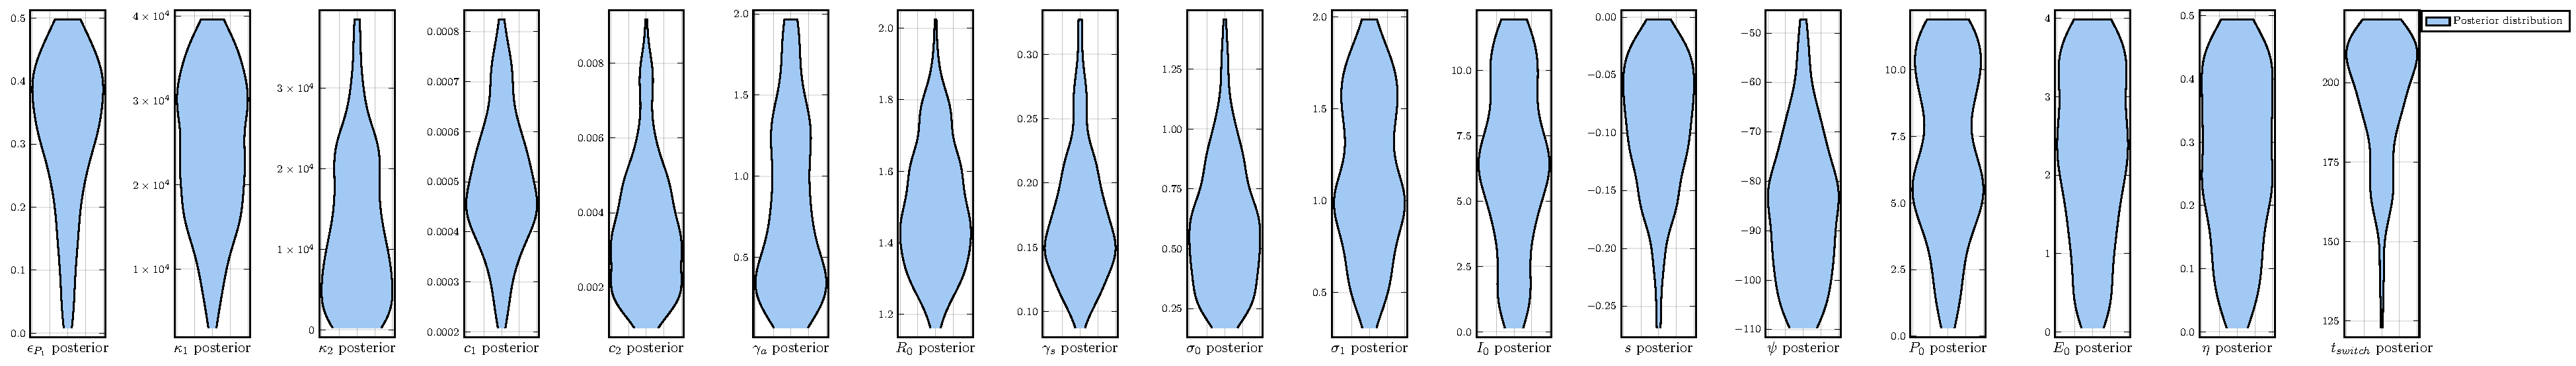
\includegraphics[width = 18 cm]{appendices/FigureS1.pdf}
\caption{\textbf{Posterior distributions on inferred non-age structured model parameters for baseline model}.Posteriors are composed of 200 candidate parameter sets from the particle filtering, the model was evaluated at these points for all future runs.}
\label{s1}
\end{figure}

\begin{figure}[H]
    \centering
    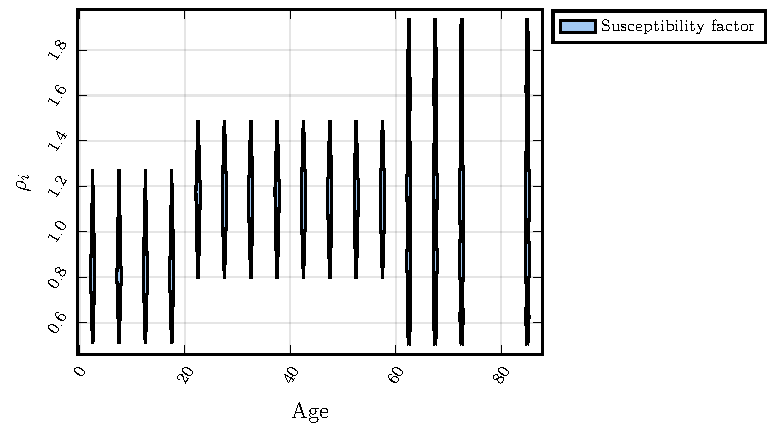
\includegraphics[width = 12 cm]{appendices/FigureS2.pdf}
    \caption{\textbf{Posterior distributions on inferred age-specific susceptibility modifier parameter $\rho_i$ for baseline model}. Three age-specific susceptibility parameters shown here, $\rho_1,\rho_2,\rho_3$, were also inferred from particle filtering on the case and mobility data, corresponding to the age brackets 0-20, 20-60, 60+.}
    \label{s2}
    \end{figure}
    
    \clearpage 
    
    \begin{figure}[H]
    \centering
    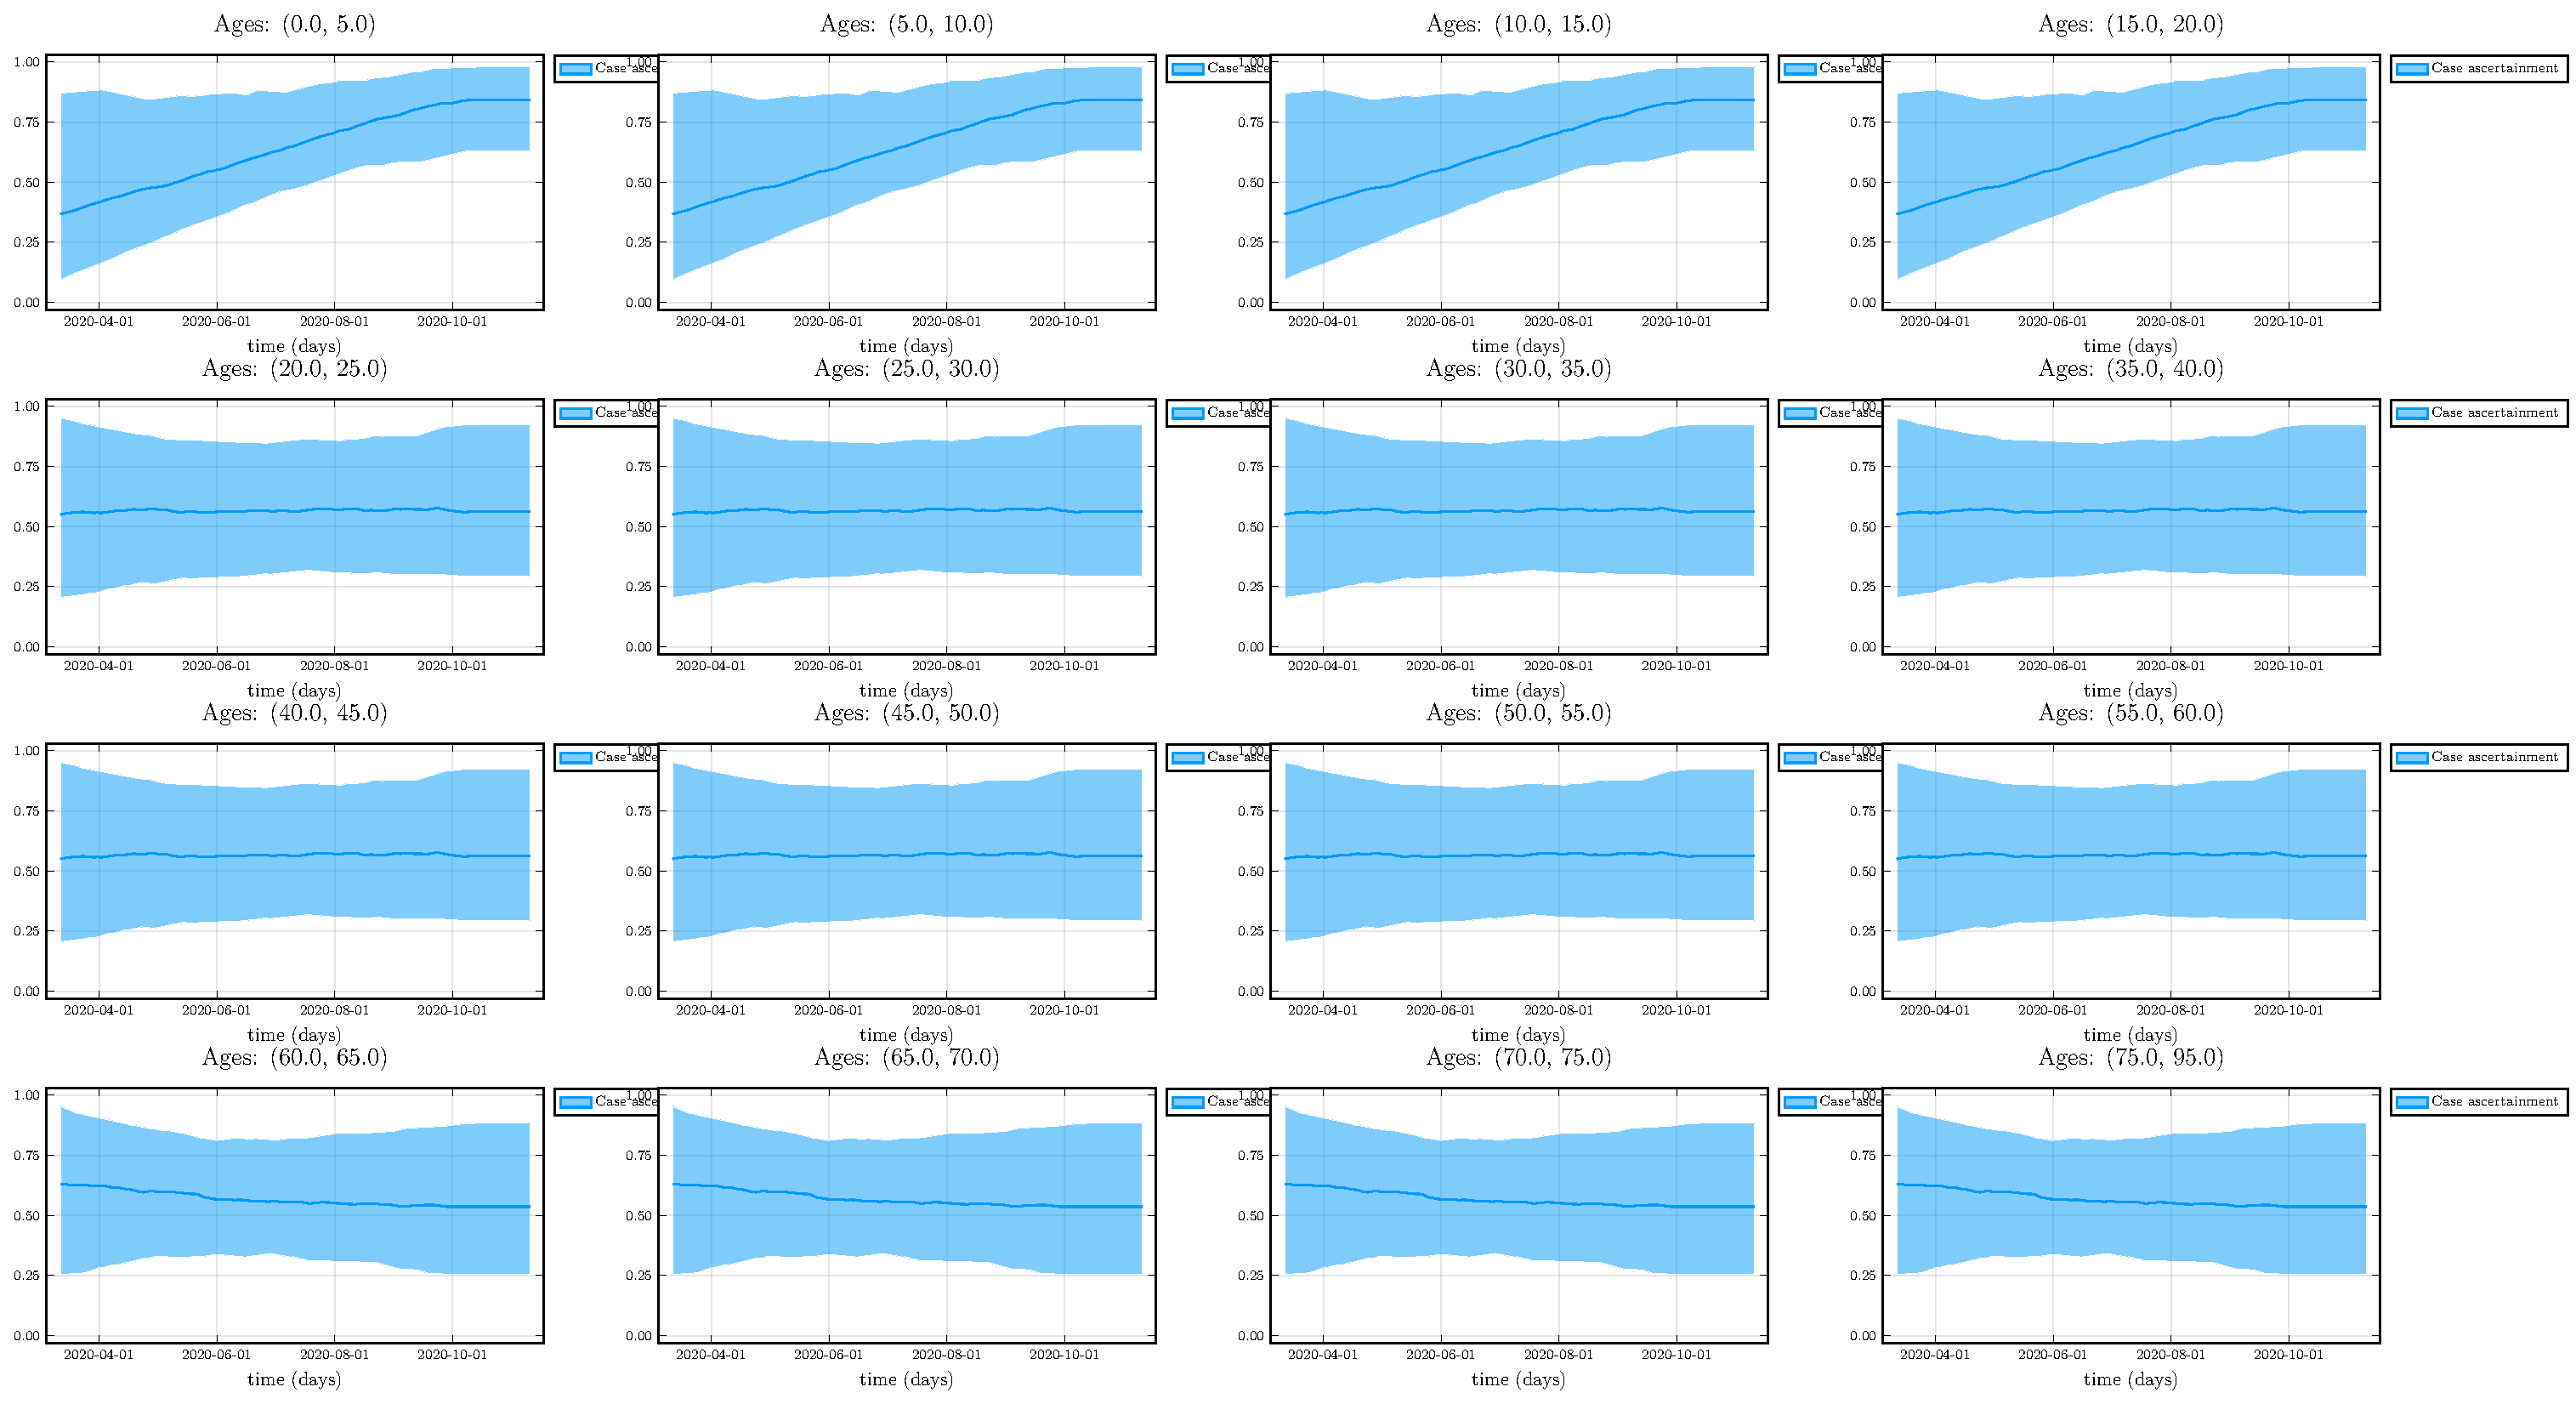
\includegraphics[width = 18 cm]{appendices/FigureS3.pdf}
    \caption{\textbf{Posterior distributions on inferred age-specific ascertainment rate over time for baseline model}. Time dependent ascertainment rates inferred from the data, corresponding to the fraction of actual cases detected by the Ontario testing system. }
    \label{s3}
    \end{figure}
    
    \clearpage 
    
    \begin{figure}[H]
    \centering
    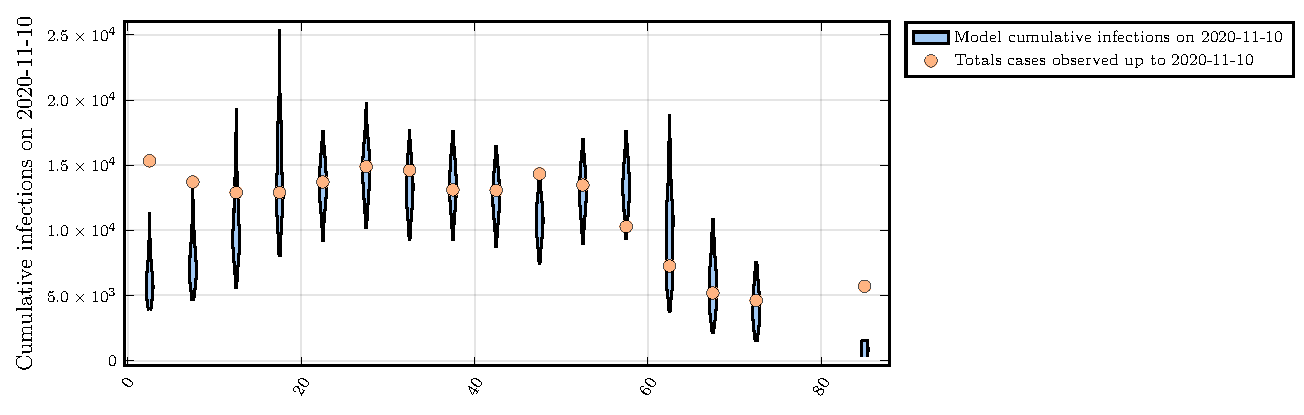
\includegraphics[width = 12 cm]{appendices/FigureS4.pdf}
    \caption{\textbf{Empirical data of cumulative infections due to COVID-19 by age and model posterior predictions.} The age-specific total cases at the end of the fitting window, were used to calibrate the model, in an age dependent way. We used only three parameters to capture age specific effects and therefore trade-off some accuracy in the youngest and oldest age groups.}
    \label{s4}
    \end{figure}
    
    \clearpage 
    
    \begin{figure}[H]
    \centering
    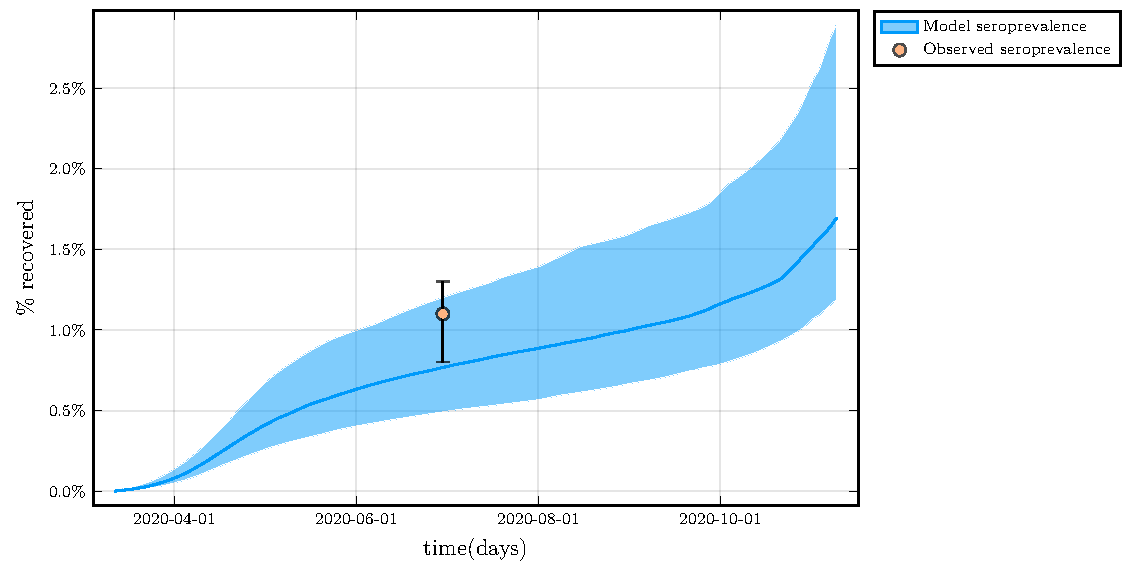
\includegraphics[width = 12 cm]{appendices/FigureS5.pdf}
    \caption{\textbf{Average of model posterior population seropositivity over time, compared to empirical data.} Total seroprevalence in Ontario was assessed during the month of June. We used this value to calibrate the model further.  }
    \label{s5}
    \end{figure}
    
    \clearpage 
    
    \begin{figure}[H]
    \centering
    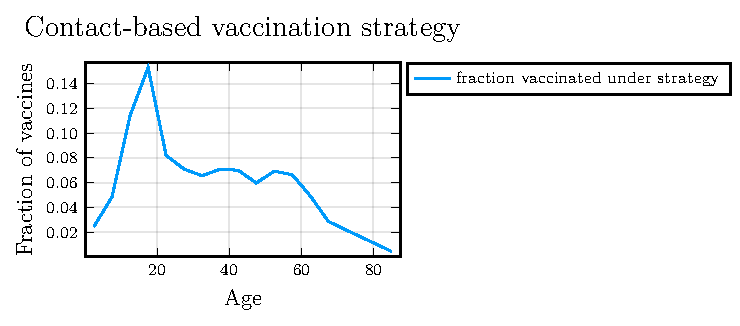
\includegraphics[width = 12 cm]{appendices/FigureS6.pdf}
    \caption{\textbf{Age distribution of vaccination under the contact-based strategy.} This strategy vaccinates proportionally to the leading eigenvector of the full contact matrix, $C(0)$, to vaccinate people who will, approximately, produce the most secondary infections in a linearized regime.}
    \label{s6}
    \end{figure}
    
    \clearpage 
    
    \begin{figure}[H]
    \centering
    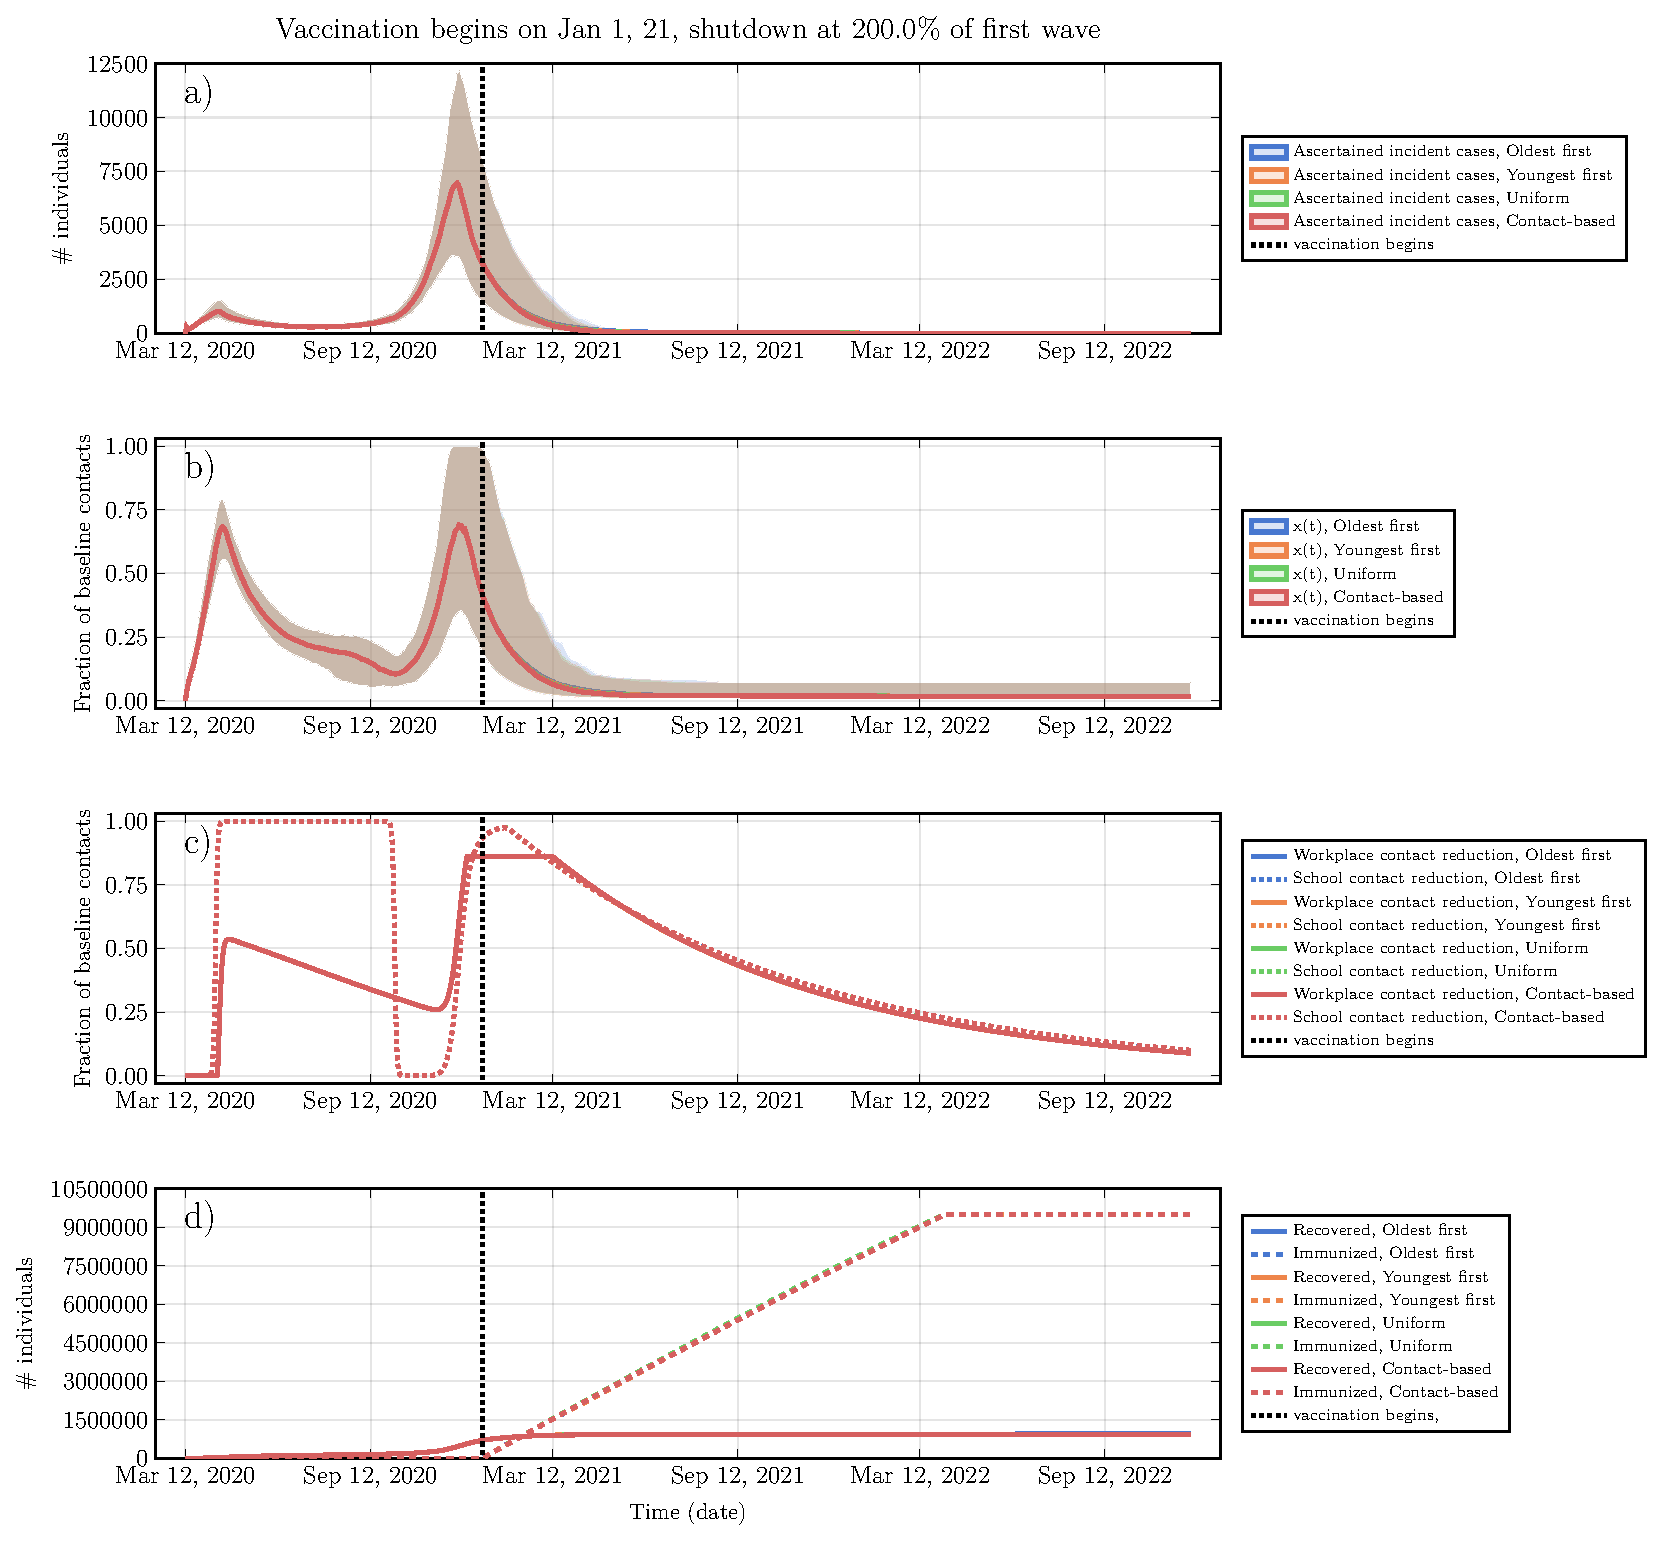
\includegraphics[width = 16 cm]{appendices/FigureS7.pdf}
    \caption{\textbf{Social and epidemic dynamics for early vaccine availability and high vaccination rate.} (a) Ascertained incident COVID-19 cases, (b) proportion $x$ of the population practicing NPIs, (c) Intensity of school and workplace closure, (d) percentage of population with natural or vaccine-derived immunity versus time. $T=200 \%$, $\psi_0=1.5 \%$ per week, vaccine available in January 2021.   Other parameters are in Table \ref{tab:params}.}
    \label{s7}
    \end{figure}
    
    \clearpage 
    
    \begin{figure}[H]
    \centering
    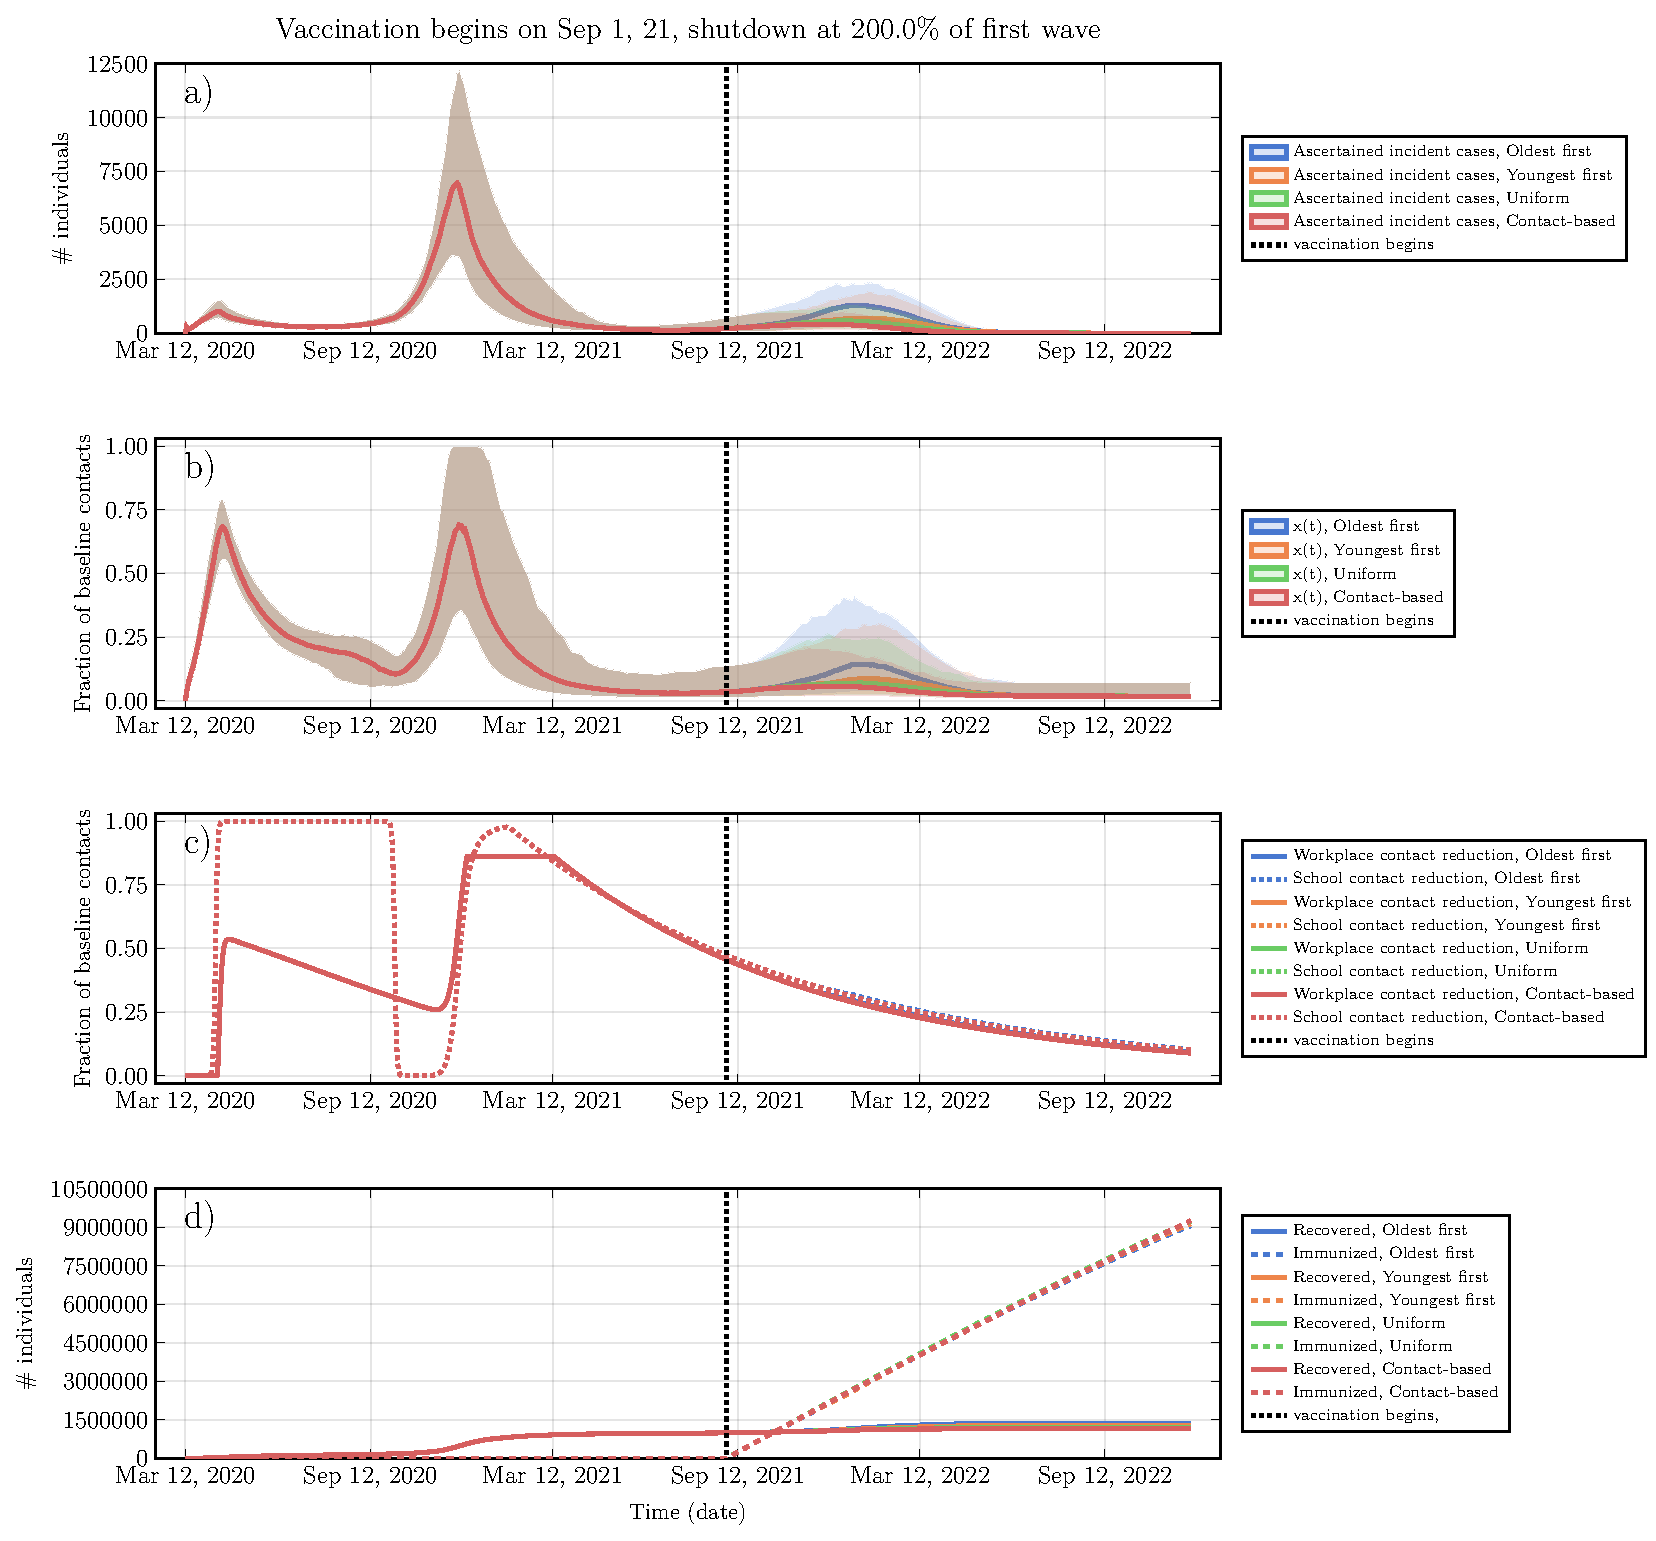
\includegraphics[width = 16 cm]{appendices/FigureS8.pdf}
    \caption{\textbf{Social and epidemic dynamics for late vaccine availability and high vaccination rate.} (a) Ascertained incident  COVID-19 cases, (b) proportion $x$ of the population practicing NPIs, (c) Intensity of school and workplace closure, (d) percentage of population with natural or vaccine-derived immunity versus time. $T=200 \%$, $\psi_0=1.5 \%$ per week, vaccine available in September 2021.   Other parameters are in Table \ref{tab:params}.}
    \label{s8}
    \end{figure}
    
    \clearpage 
    
    \begin{figure}[H]
    \centering
    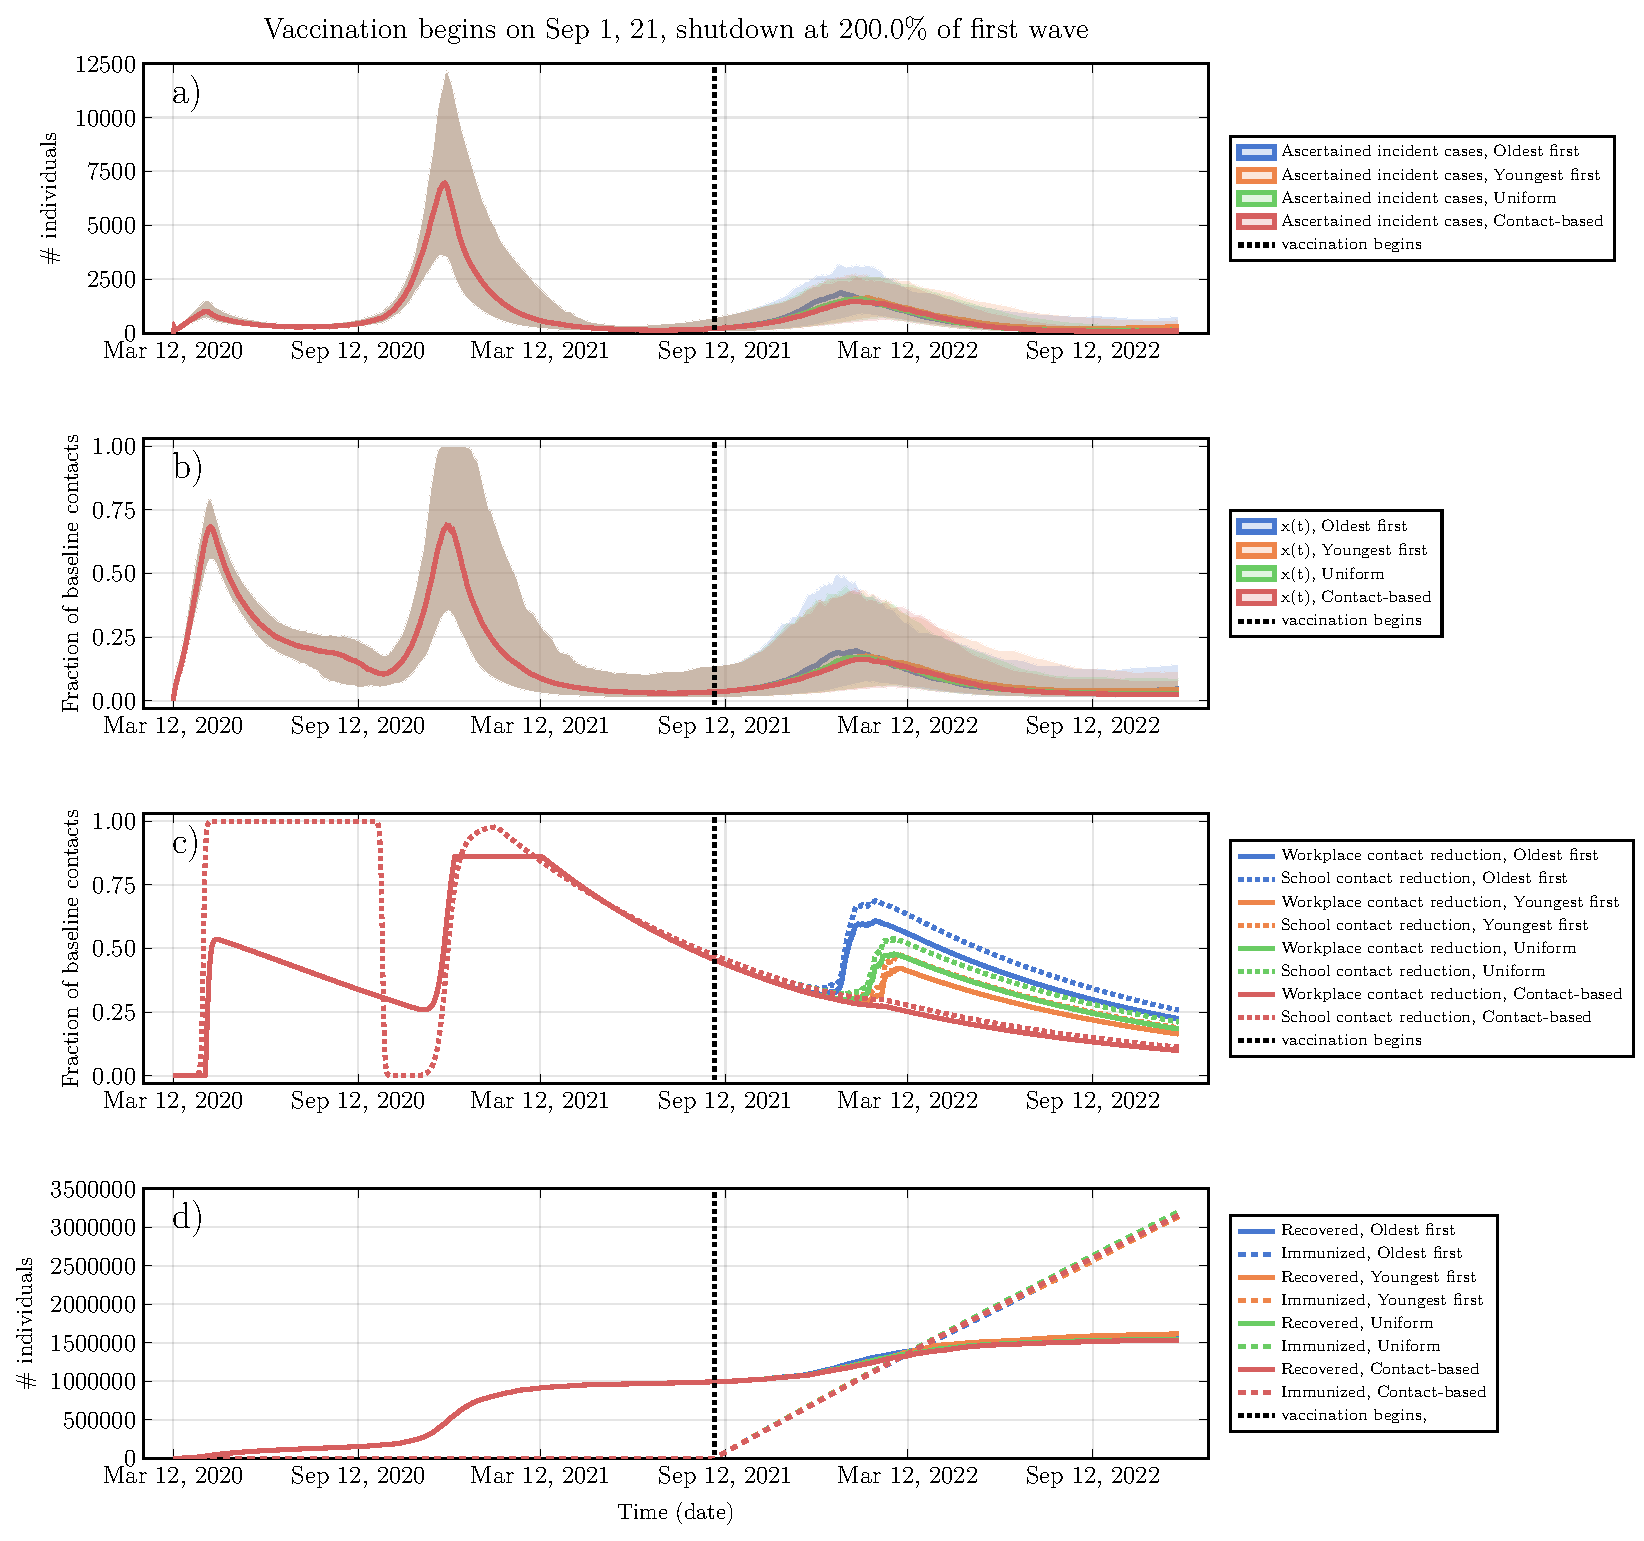
\includegraphics[width = 16 cm]{appendices/FigureS9.pdf}
    \caption{\textbf{Social and epidemic dynamics for late vaccine availability and low vaccination rate.} (a) Ascertained incident COVID-19 cases, (b) proportion $x$ of the population practicing NPIs, (c) Intensity of school and workplace closure, (d) percentage of population with natural or vaccine-derived immunity versus time. $T=200 \%$, $\psi_0=0.5 \%$ per week, vaccine available in September 2021.   Other parameters are in Table \ref{tab:params}.}
    \label{s9}
    \end{figure}
    
    
    \clearpage 
    
    \begin{figure}[H]
    \centering
    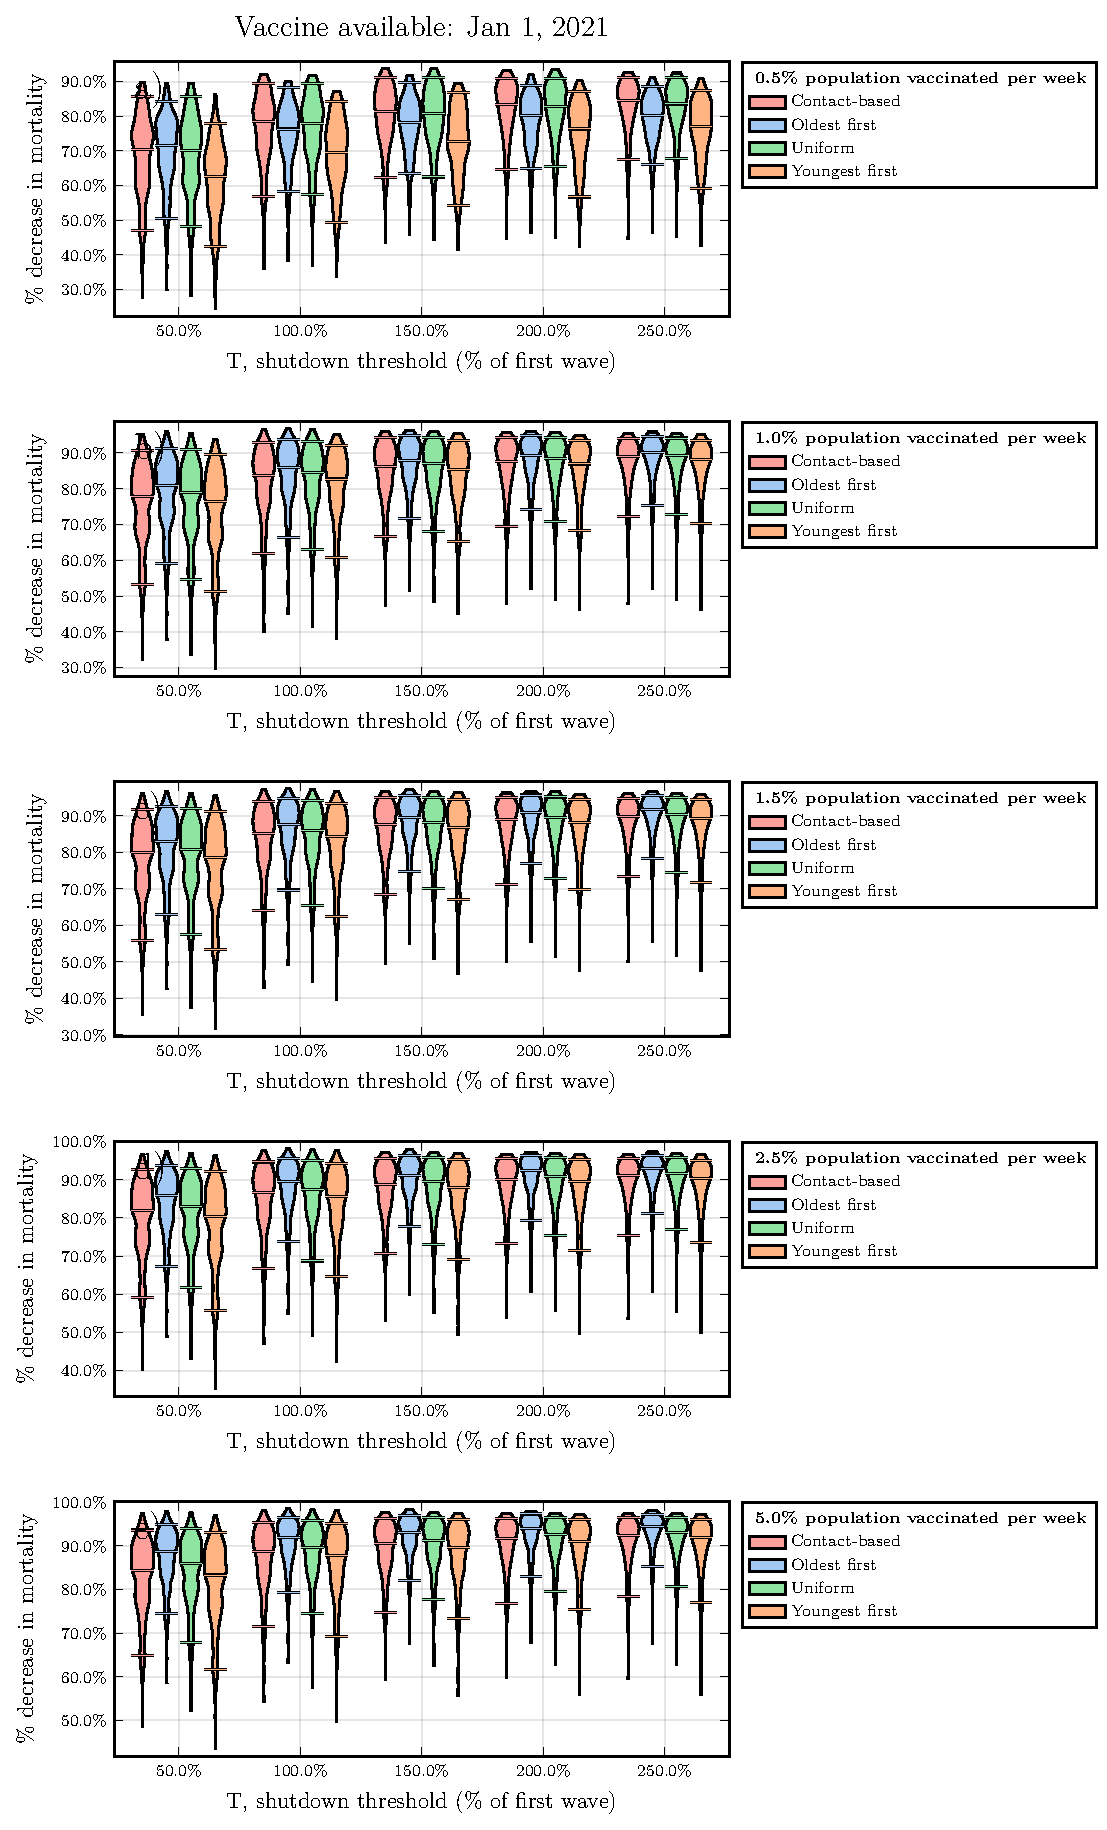
\includegraphics[width = 12 cm]{appendices/FigureS10.pdf}
    \caption{\textbf{Mortality reductions under various values of $T$ and $\psi_0$, early vaccine availability.} Violin plots of the percent reduction in mortality under the four vaccine strategies, relative to no vaccination, as a function of the vaccination rate $\psi_0$, for January 2021 availability. Horizontal lines represent median values of posterior model projections. Other parameter values in Table S1.  Percentage reductions are relative to no vaccination.  Projected number of deaths in the absence of vaccination were 35597.2 (CI: 57465.9,19507.9); 48518.8 (CI: 86853.9,28335.7), 61339.1 (CI: 106623.0,34613.5), 
    72007.3 (CI: 121754.0,40483.4); 80707.6 (CI: 126732.0,47755.4) after January 1, 2021, for T=50\%, 100\%, 150\%, 200\%, and 250\%, respectively. }
    \label{s10}
    \end{figure}
    
    
    
    
    \clearpage 
    
    
    \begin{figure}[H]
    \centering
    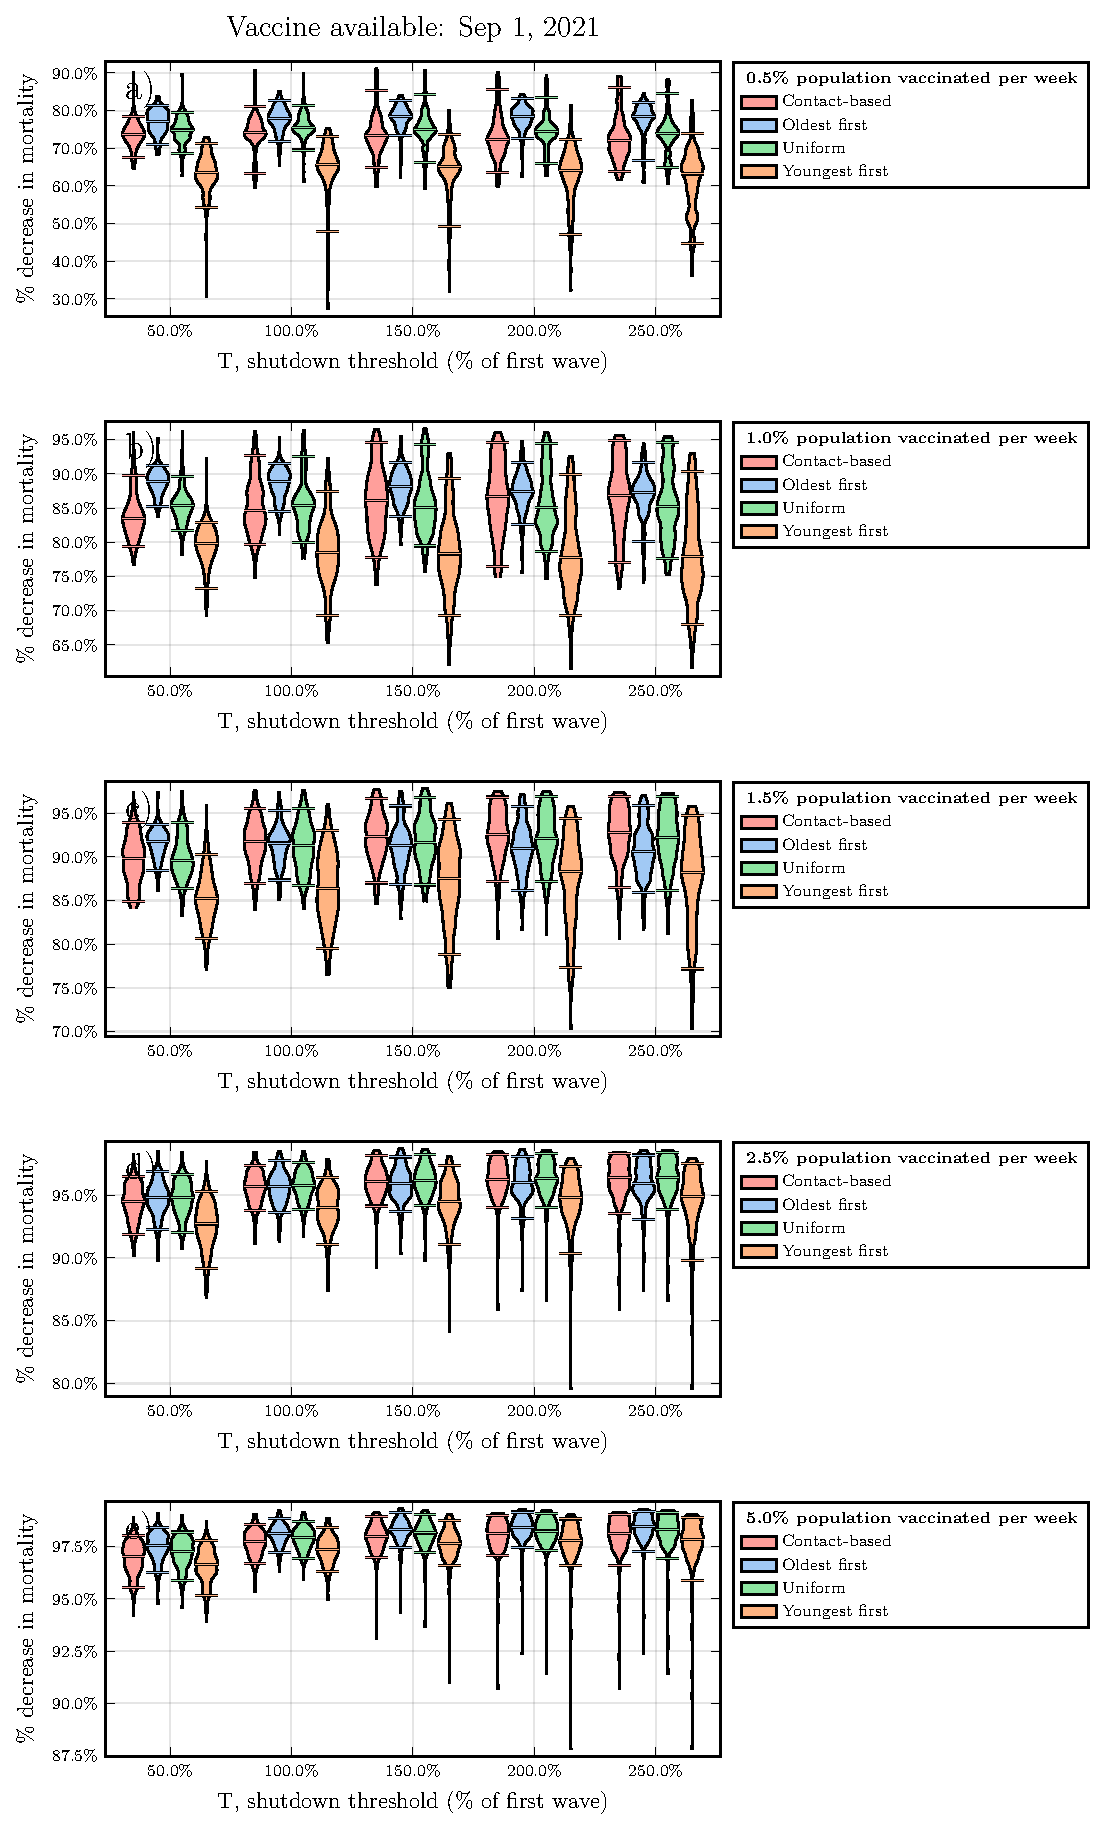
\includegraphics[width = 12 cm]{appendices/FigureS11.pdf}
    \caption{\textbf{Mortality reductions under various values of $T$ and $\psi_0$, late vaccine availability.} Violin plots of the percent reduction in mortality under the four vaccine strategies, relative to no vaccination, as a function of the vaccination rate $\psi_0$, for September 2021 availability. Horizontal lines represent median values of posterior model projections. Other parameter values in Table S1.  Percentage reductions are relative to no vaccination. Projected number of deaths in the absence of vaccination were 25478.8 (CI: 45679.0,13006.7); 39149.6 (CI: 73917.1,20290.9); 50775.1 (CI: 95451.2,25980.9); 60250.7 (CI: 108361.0,30721.9); 68594.0 (CI: 107157.0,36063.6) after September 1, 2021 for T=50\%, 100\%, 150\%, 200\%, and 250\%, respectively. }
    \label{s11}
    \end{figure}
    
    
    
    \clearpage 
    
    
    \begin{figure}[H]
    \centering
    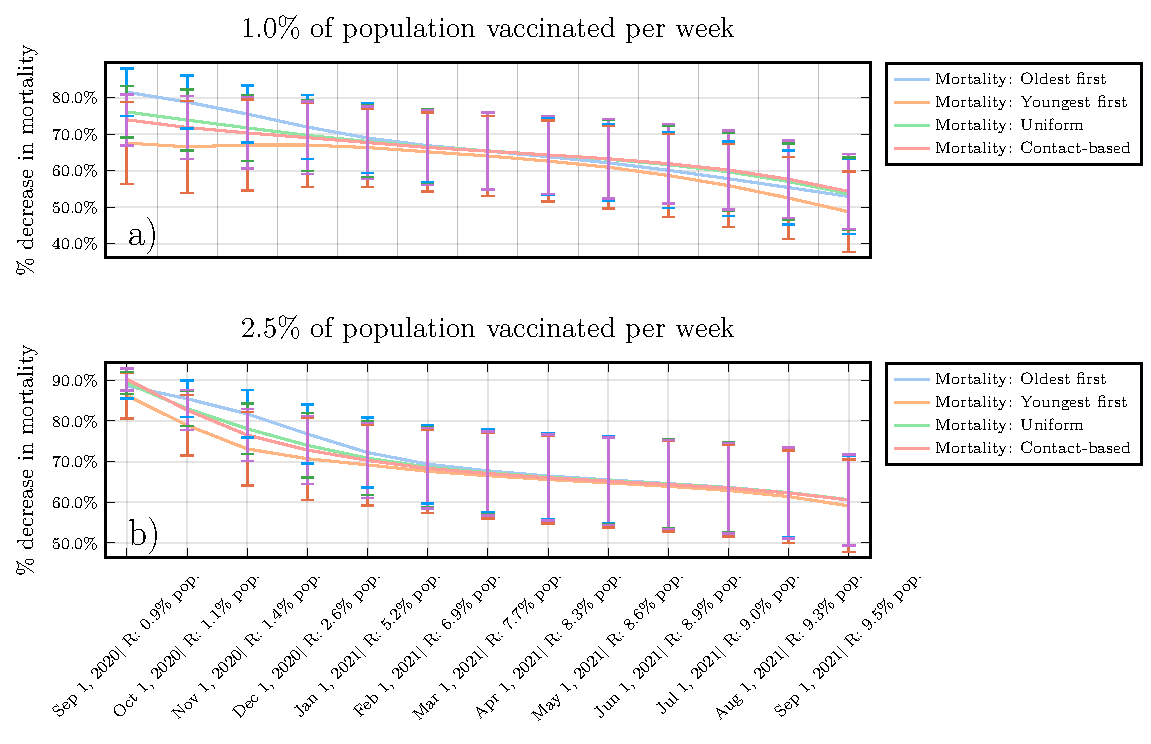
\includegraphics[width = 15 cm]{appendices/FigureS12.pdf}
    \caption{\textbf{A higher level of natural immunity increases the relative advantage of transmission-interrupting strategies.}  Median and standard deviation of the percent reduction in mortality under the four vaccine strategies, relative to no vaccination, as a function of the vaccination start date and percent recovered at that time, for (a) $\phi_0=1.0 \%$ vaccinated per week and (b) $\phi_0=2.5 \%$ vaccinated per week.  Shutdown threshold $T=200 \%$,  and other parameter values in Appendix, Table S1.}
    \label{s12}
    \end{figure}
    
    \clearpage 
    
    \begin{figure}[H]
    \centering
    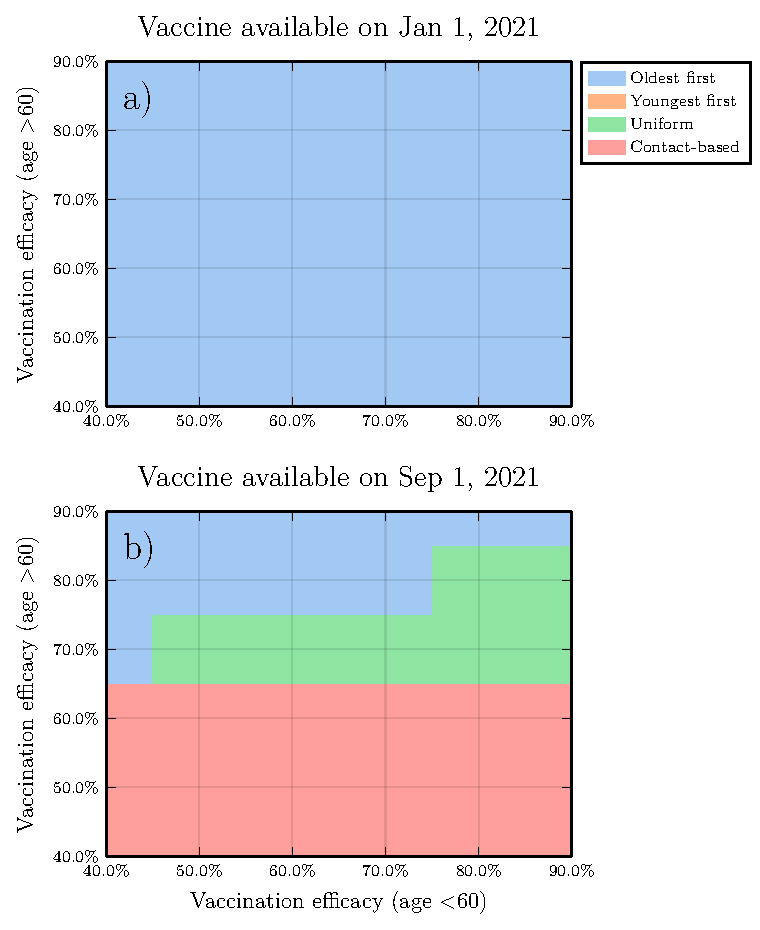
\includegraphics[width = 14 cm]{appendices/FigureS13.pdf}
    \caption{\textbf{Sensitivity analysis exploring a range of vaccine efficacy values, for vaccination rate $\phi_0=2.5 \%$ per week.} Subpanels are parameter planes for January and September availability showing the vaccination strategy that reduces COVID-19 mortality the most as a function of vaccine efficacy in $60+$ year-olds versus vaccine efficacy in other age groups. Other parameter values as in Table S1.}
    \label{s13}
    \end{figure}
    
    \clearpage 
    
    \begin{figure}[H]
    \centering
    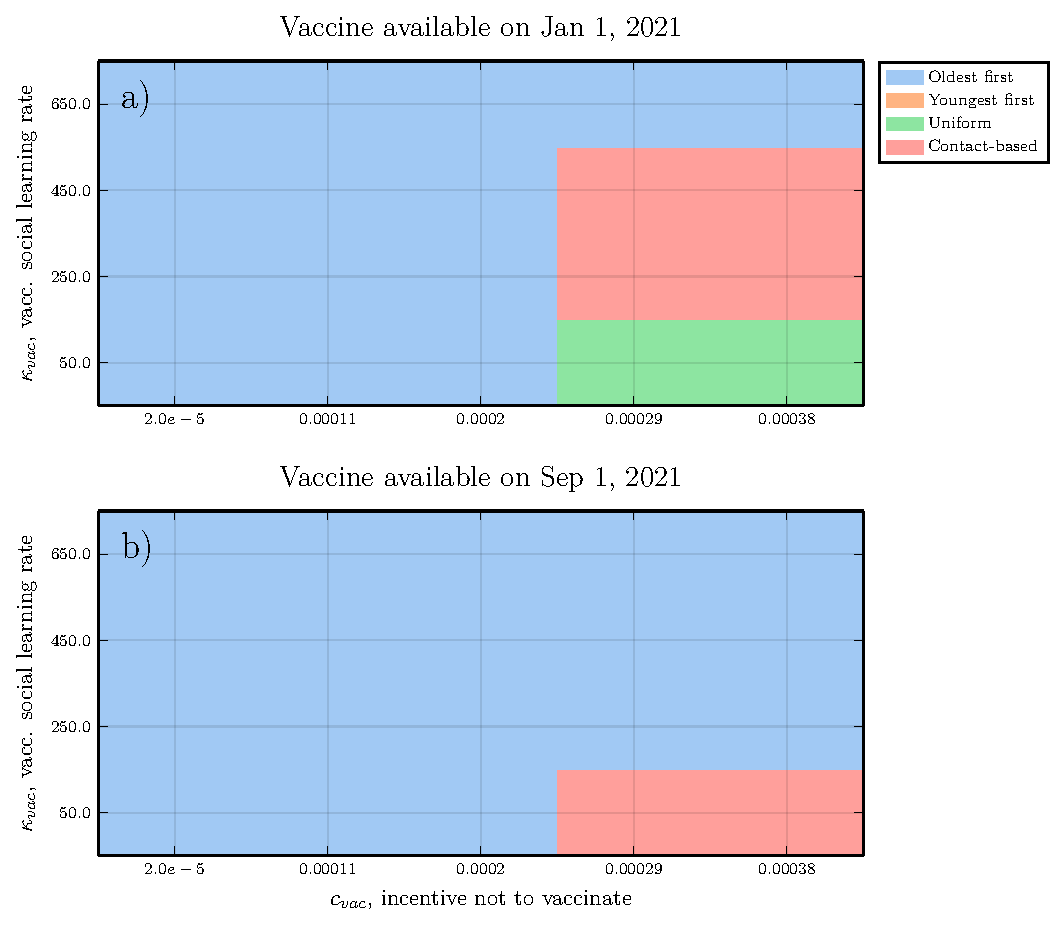
\includegraphics[width = 14 cm]{appendices/FigureS14.pdf}
    \caption{\textbf{Sensitivity analysis exploring impact of vaccinating behaviour dynamics.} $\phi_0 = 2.5 \%$ per week, $T=200 \%$. Subpanels are parameter planes for January and September availability showing the vaccination strategy that reduces COVID-19 mortality the most as a function of vaccine social learning rate $\kappa_{vac}$ and vaccine cost parameter $c_{vac}$. Other parameter values as in Table S1.}
    \label{s14}
    \end{figure}
    
    \clearpage 
    
    \begin{figure}[H]
    \centering
    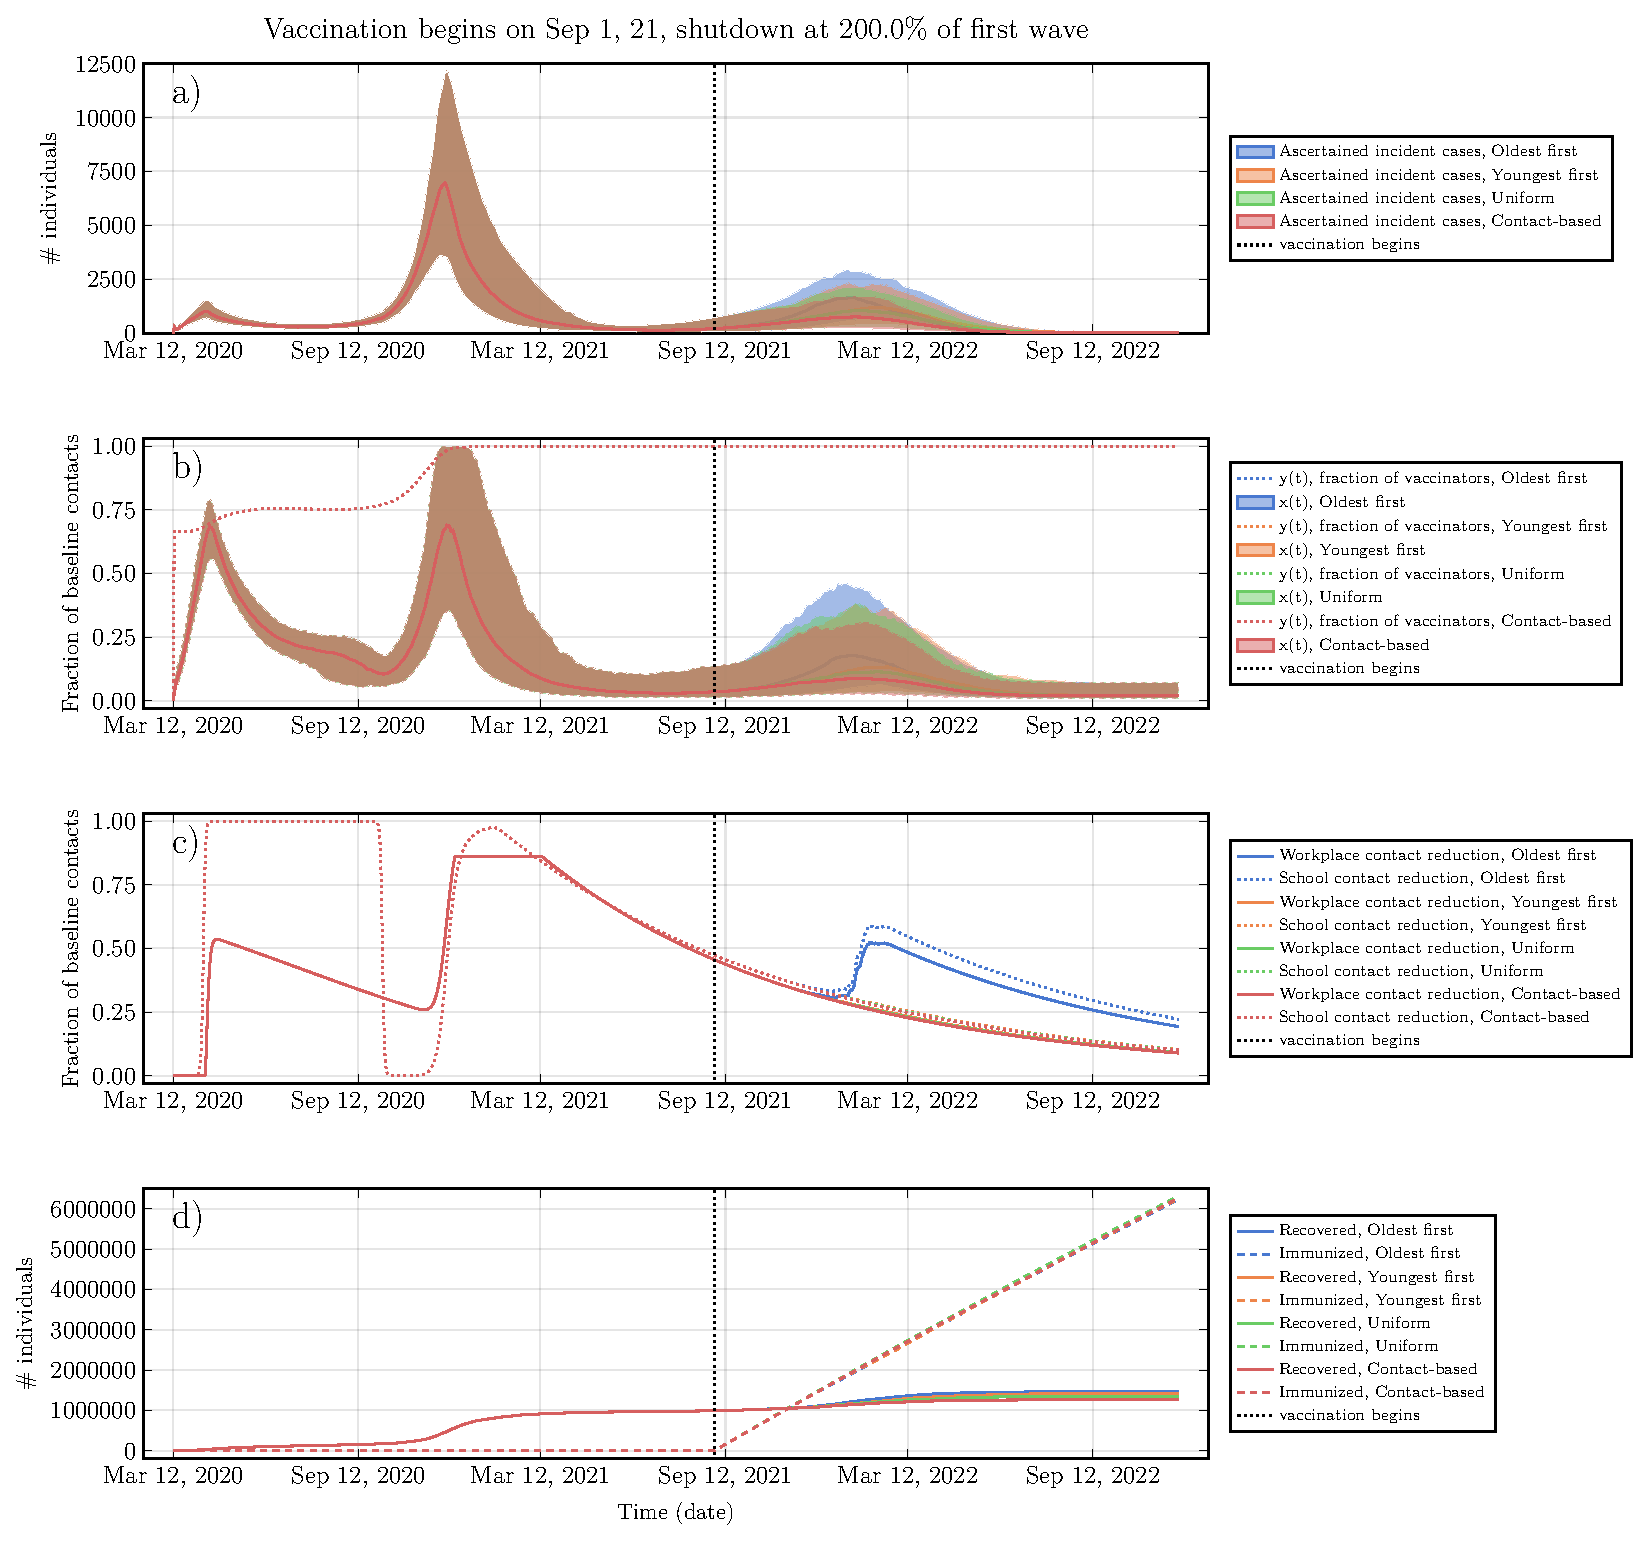
\includegraphics[width = 16 cm]{appendices/FigureS15.pdf}
    \caption{\textbf{Epidemic dynamics and social dynamics for both NPI adherence and vaccinating behaviour, when vaccine cost is small, $c_{vac}=1.1\times 10^{-4}$.} (a) Ascertained incident COVID-19 cases, (b) proportion $x$ of the population practicing NPIs, (c) Intensity of school and workplace closure, (d) percentage of population with natural or vaccine-derived immunity versus time. $T=200 \%$, $\psi_0=1.0 \%$ per week (maximum rate in absence of vaccine refusal), vaccine available in September 2021, $\kappa_{vac}=50$/day.   Other parameters are in Table \ref{tab:params}.}
    \label{s15}
    \end{figure}
    
    \clearpage 
    
    \begin{figure}[H]
    \centering
    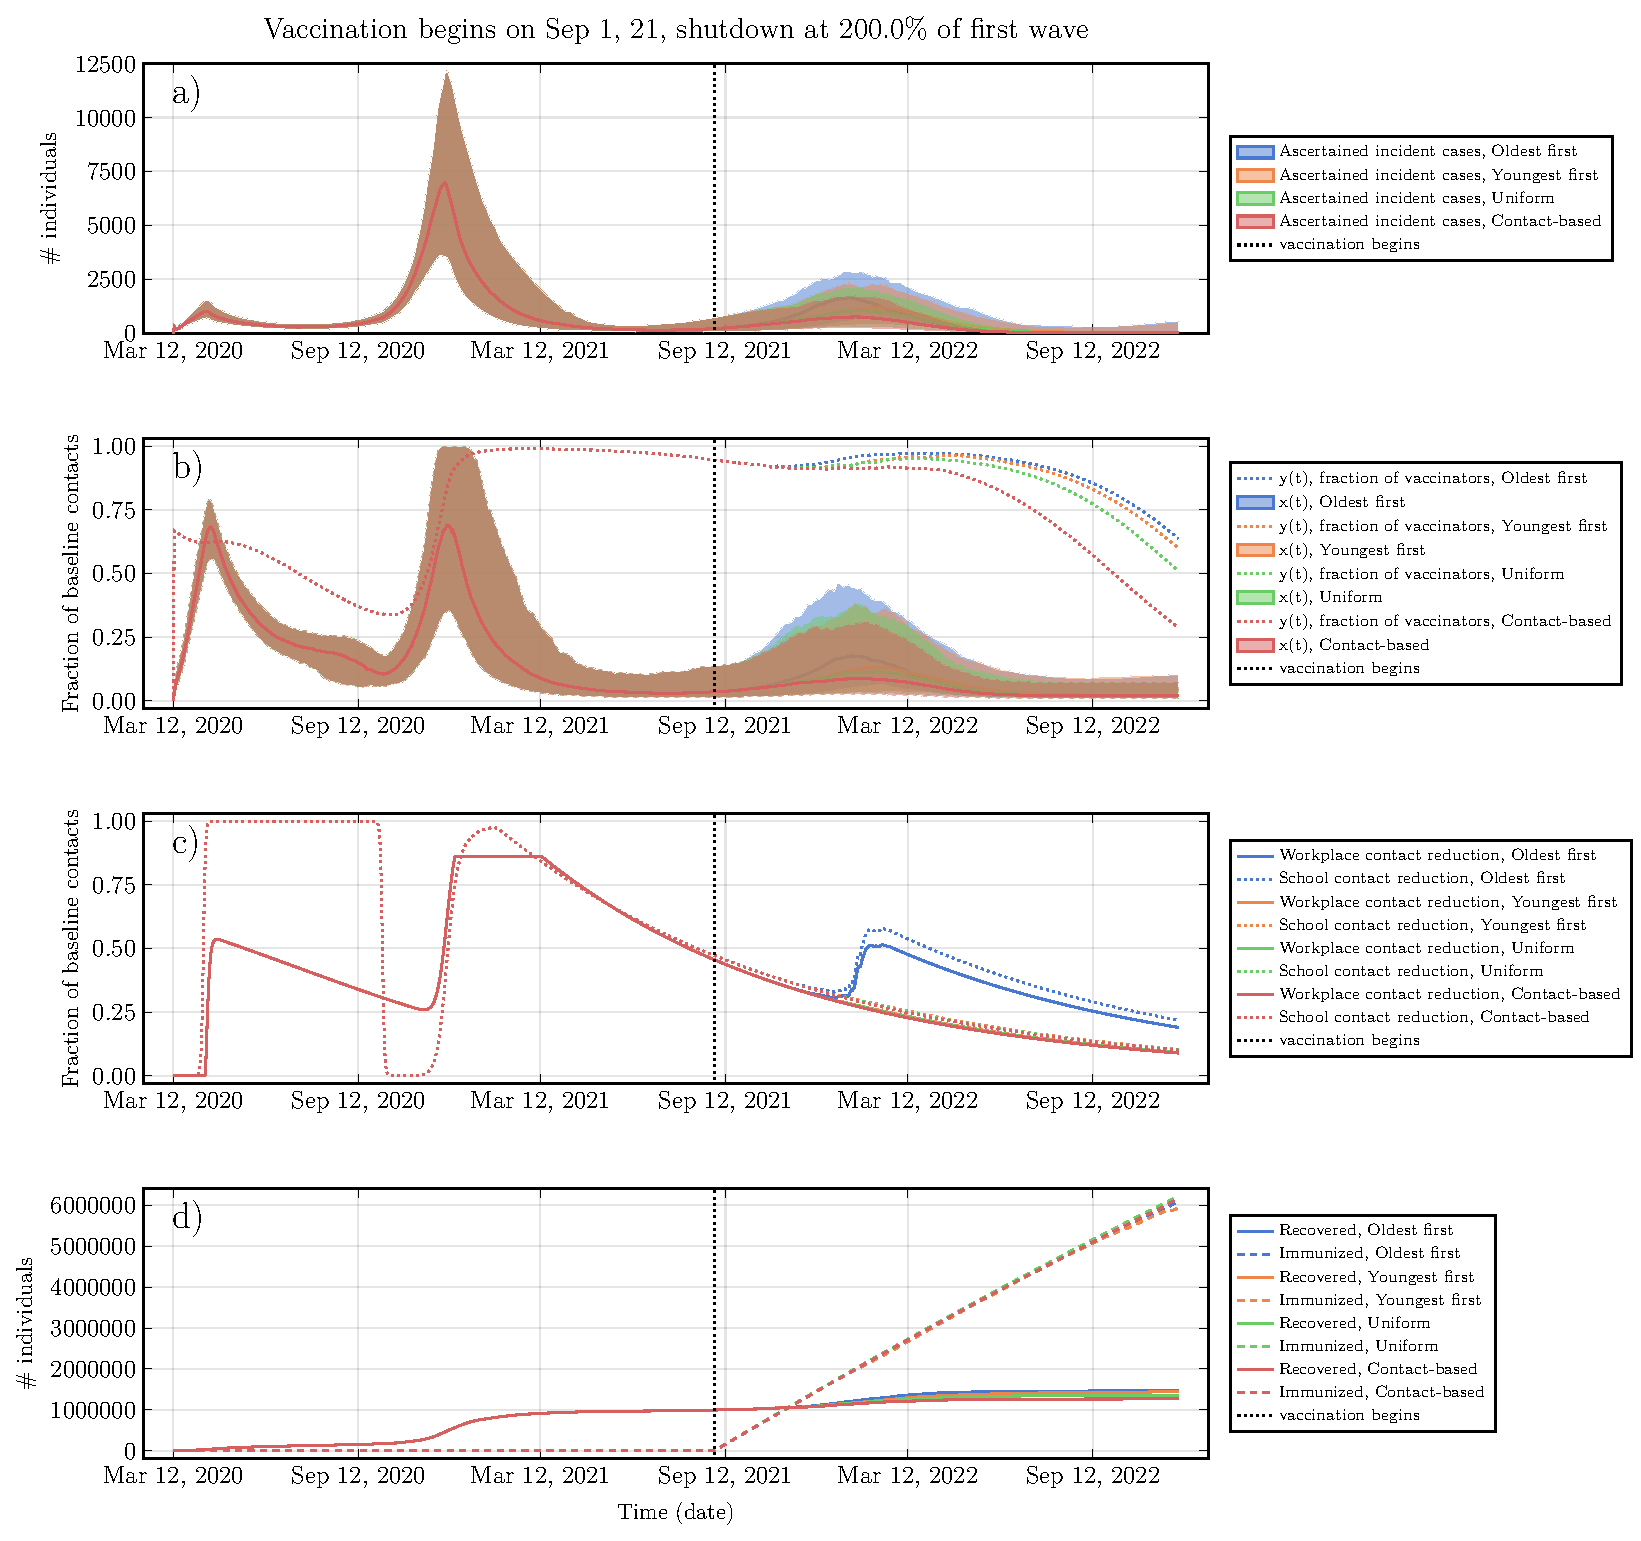
\includegraphics[width = 16 cm]{appendices/FigureS16.pdf}
    \caption{\textbf{Epidemic dynamics and social dynamics for both NPI adherence and vaccinating behaviour, when vaccine cost is moderate, $c_{vac}=2.9\times 10^{-4}$.} (a) Ascertained incident COVID-19 cases, (b) proportion $x$ of the population practicing NPIs, (c) Intensity of school and workplace closure, (d) percentage of population with natural or vaccine-derived immunity versus time. $T=200 \%$, $\psi_0=1.0 \%$ per week (maximum rate in absence of vaccine refusal), vaccine available in September 2021, $\kappa_{vac}=50$/day.   Other parameters are in Table \ref{tab:params}.}
    \label{s16}
    \end{figure}
    
    \clearpage 
    
    \begin{figure}[H]
    \centering
    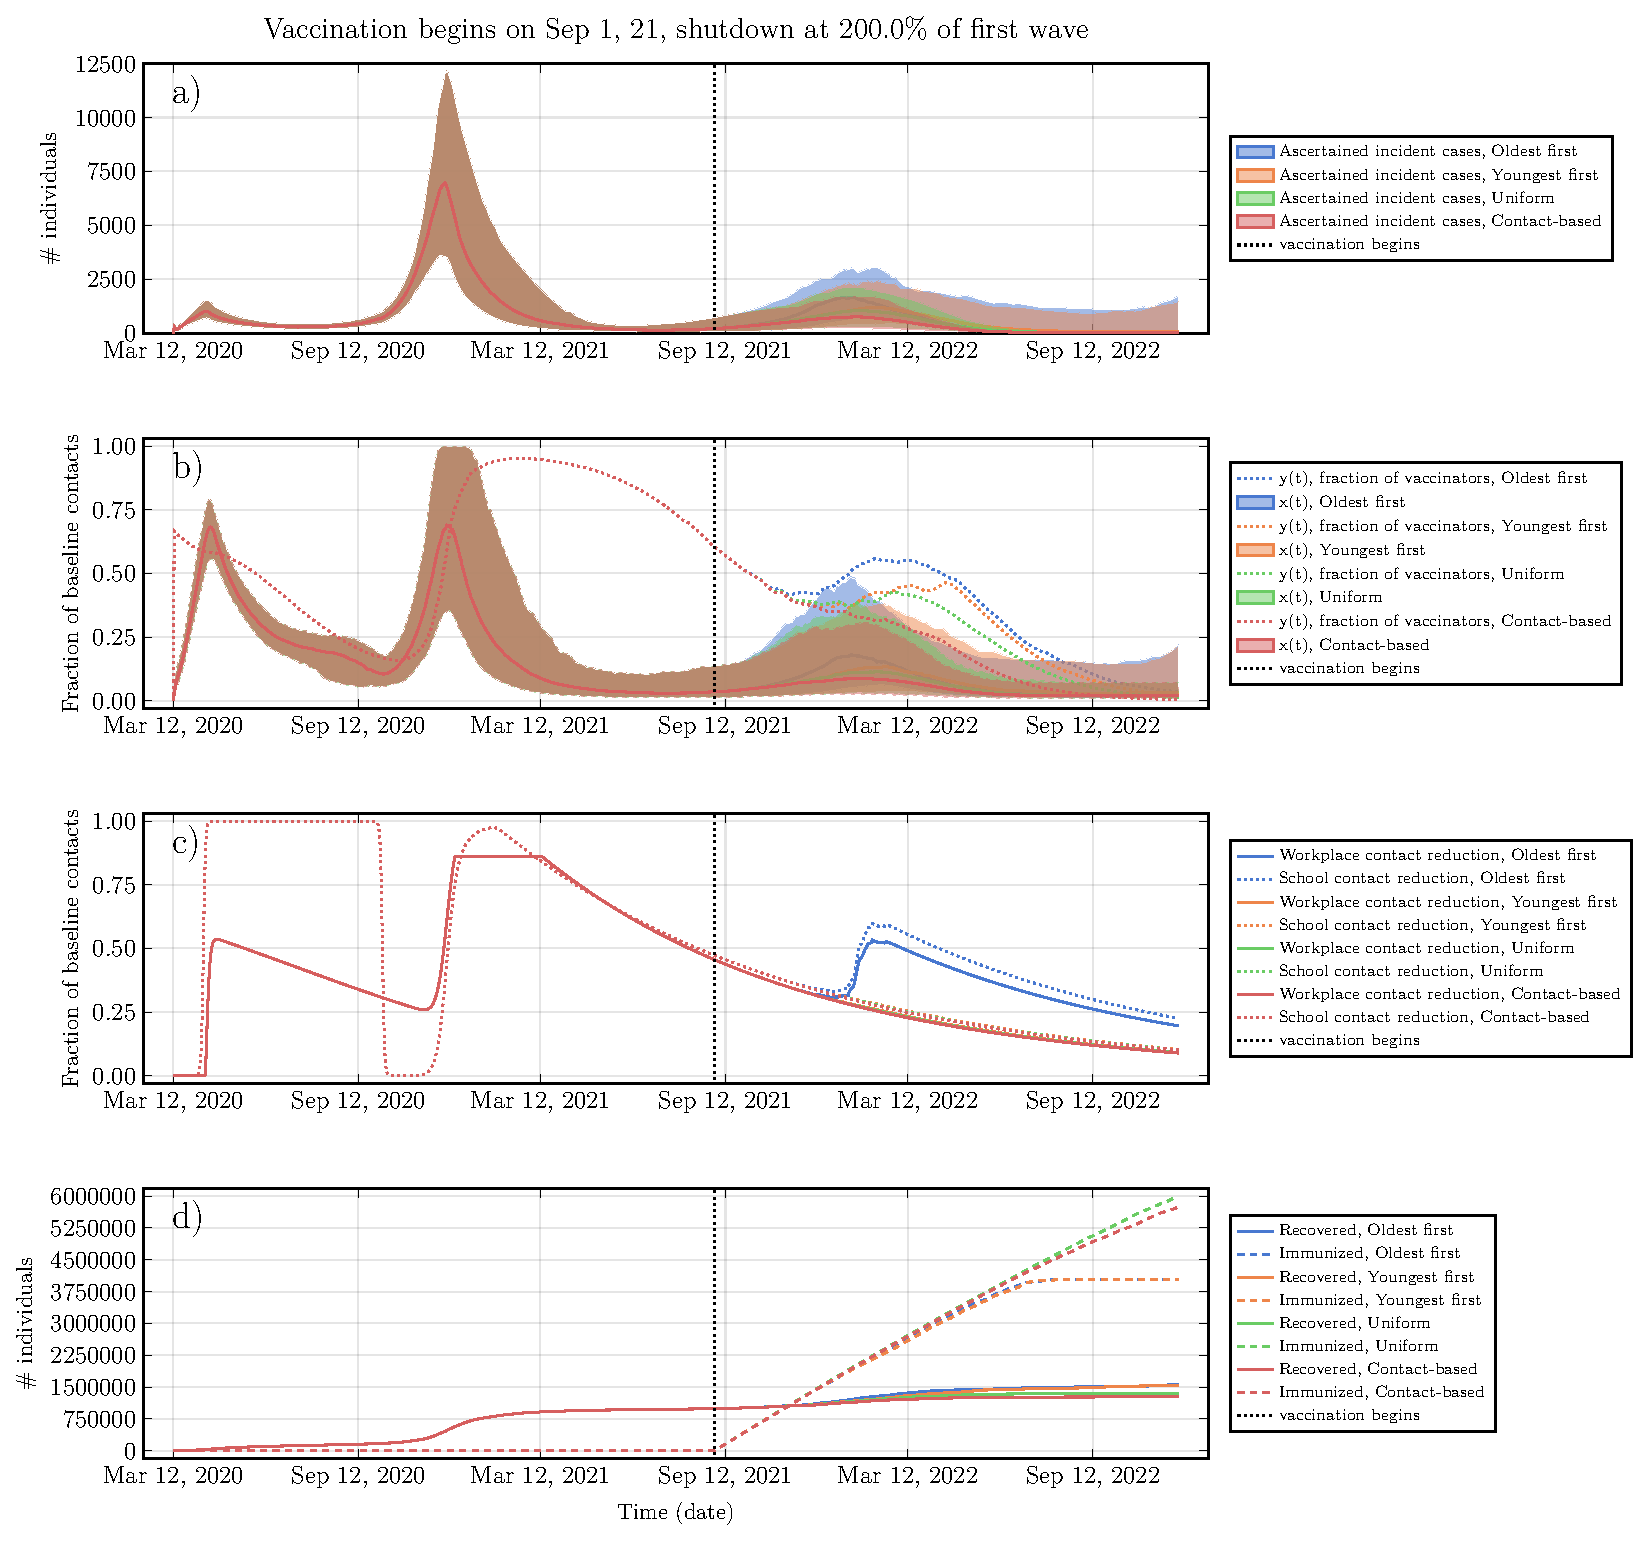
\includegraphics[width = 16 cm]{appendices/FigureS17.pdf}
    \caption{\textbf{Epidemic dynamics and social dynamics for both NPI adherence and vaccinating behaviour, when vaccine cost is high, $c_{vac}=3.8\times 10^{-4}$.} (a) Ascertained incident COVID-19 cases, (b) proportion $x$ of the population practicing NPIs, (c) Intensity of school and workplace closure, (d) percentage of population with natural or vaccine-derived immunity versus time. $T=200 \%$, $\psi_0=1.0 \%$ per week (maximum rate in absence of vaccine refusal), vaccine available in September 2021, $\kappa_{vac}=50$/day. Other parameters are in Table \ref{tab:params}.}
    \label{s17}
    \end{figure}
    
    \clearpage 
    
    \begin{figure}[H]
    \centering
    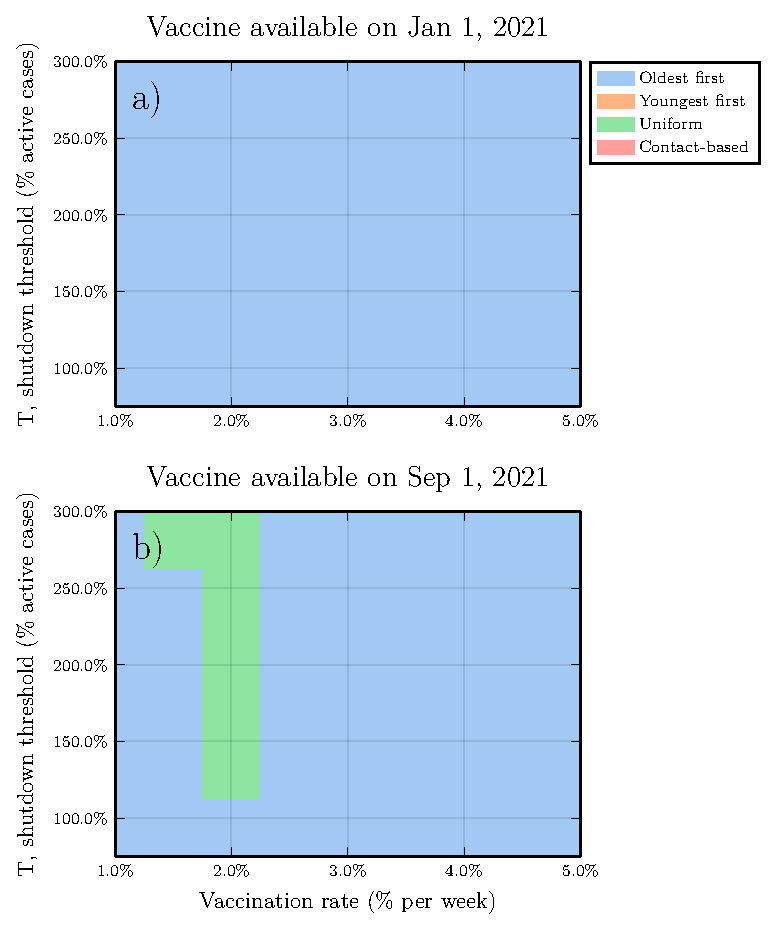
\includegraphics[width = 14 cm]{appendices/FigureS18.pdf}
    \caption{\textbf{Sensitivity analysis for the scenario where $R_0=2.5$ for December 2020 onward.} Subpanels are (left) parameter planes for January and September availability showing the vaccination strategy that prevents the most COVID-19 deaths as a function of $T$ and $\psi_0$, and (right) percentage reductions in mortality. Other parameter values are as in Table S1.}
    \label{s18}
    \end{figure}
    
    \clearpage 
    
    \begin{figure}[H]
    \centering
    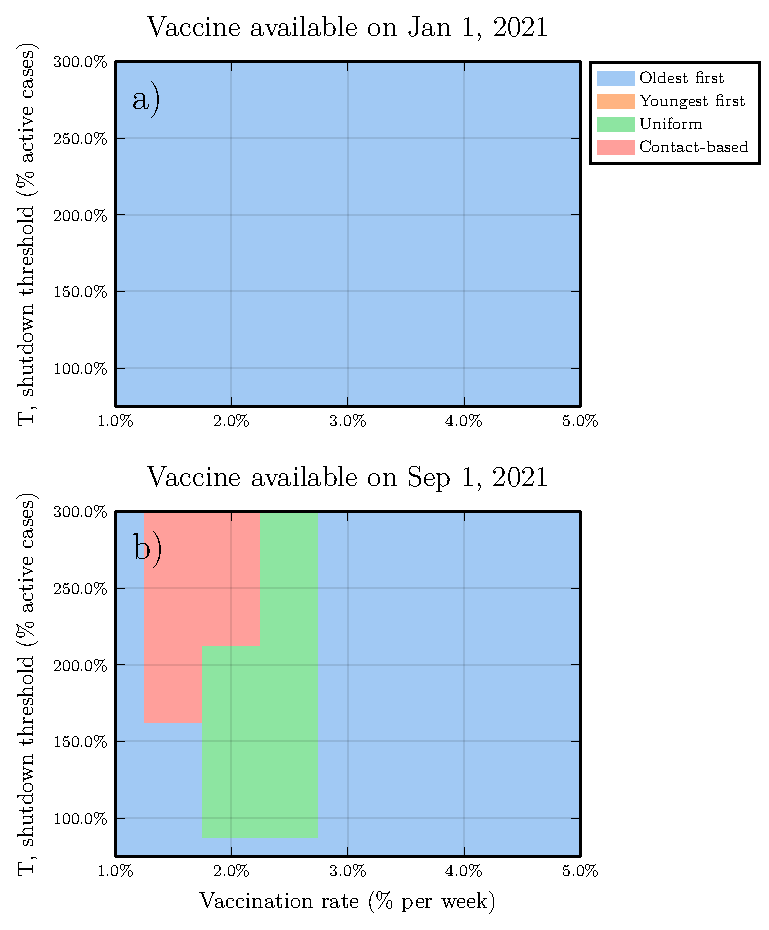
\includegraphics[width = 14 cm]{appendices/FigureS19.pdf}
    \caption{\textbf{Sensitivity analysis for the scenario of $30 \%$ heightened ascertainment across all ages from December 2020 onward.} Subpanels are parameter planes for January and September availability showing the vaccination strategy that reduces COVID-19 mortality the most as a function of $T$ and $\psi_0$ (left) and the corresponding posterior parameter distributions for the refitted parameters (right).  Other parameter values as in Table S1.}
    \label{s19}
    \end{figure}
    
    \clearpage 
    
    \begin{figure}[H]
    \centering
    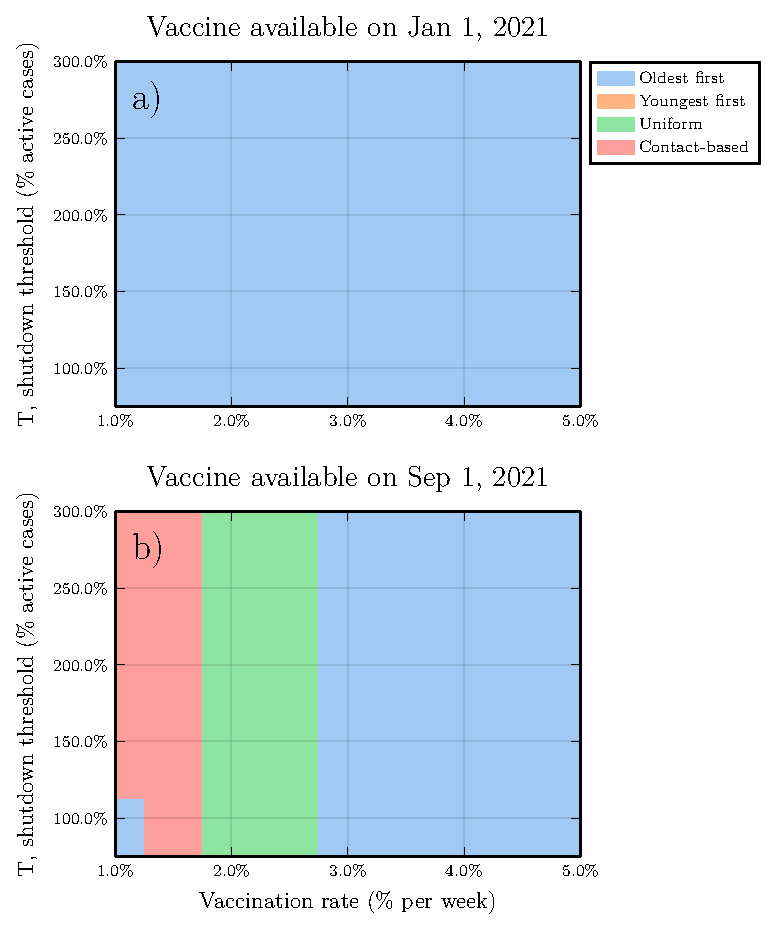
\includegraphics[width = 14 cm]{appendices/FigureS20.pdf}
    \caption{\textbf{Sensitivity analysis for the scenario of $30 \%$ reduced ascertainment across all ages from December 2020 onward.} Subpanels are parameter planes for January and September availability showing the vaccination strategy that reduces COVID-19 mortality the most as a function of $T$ and $\psi_0$ (left) and the corresponding posterior parameter distributions for the refitted parameters (right).  Other parameter values as in Table S1.}
    \label{s20}
    \end{figure}
    
    \clearpage 
    
    
    \begin{figure}[H]
    \centering
    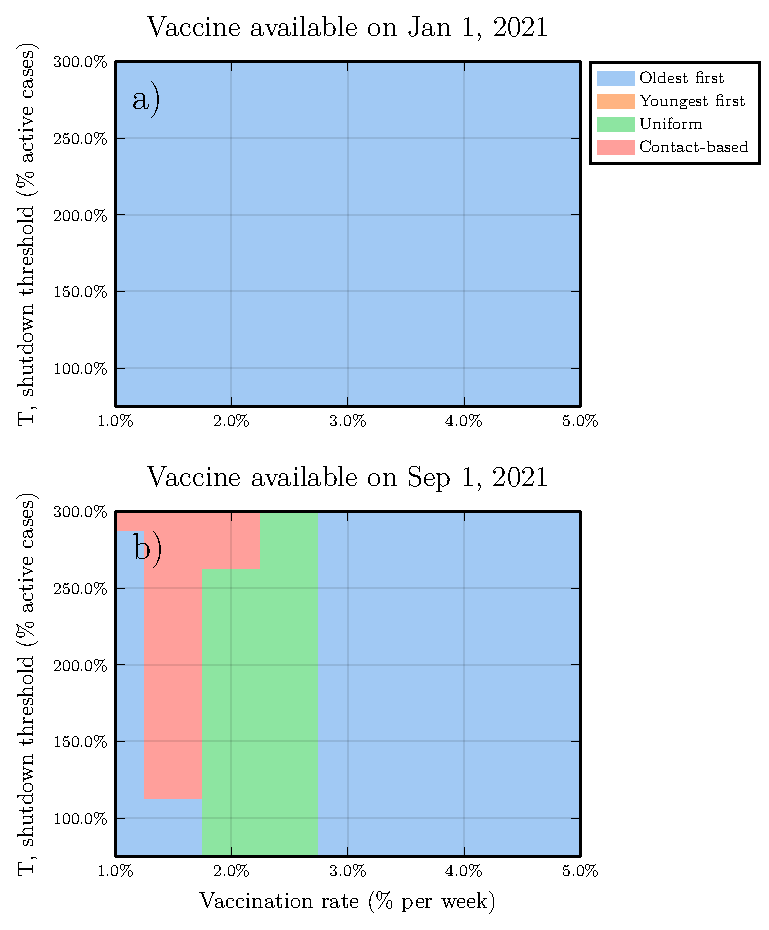
\includegraphics[width = 14 cm]{appendices/FigureS21.pdf}
    \caption{\textbf{Sensitivity analysis for the scenario of four times the baseline social learning rate from December 2020 onward.} Subpanels are parameter planes for January and September availability showing the vaccination strategy that reduces COVID-19 mortality the most as a function of $T$ and $\psi_0$ (left) and the corresponding posterior parameter distributions for the refitted parameters (right).  Other parameter values as in Table S1.}
    \label{s21}
    \end{figure}
    
    \clearpage 
    
    \begin{figure}[H]
    \centering
    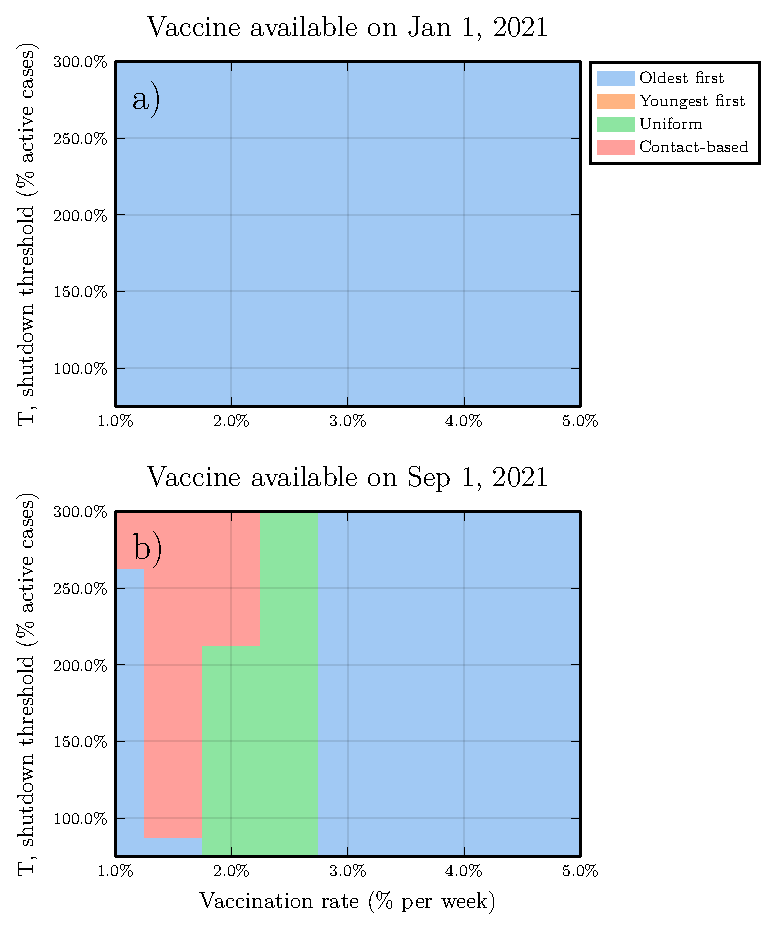
\includegraphics[width = 14 cm]{appendices/FigureS22.pdf}
    \caption{\textbf{Sensitivity analysis for the scenario of one-fourth the baseline social learning rate from December 2020 onward.} Subpanels are parameter planes for January and September availability showing the vaccination strategy that reduces COVID-19 mortality the most as a function of $T$ and $\psi_0$.  Other parameter values as in Table S1.}
    \label{s22}
    \end{figure}
    
    \clearpage 
    
    \begin{figure}[H]
    \centering
    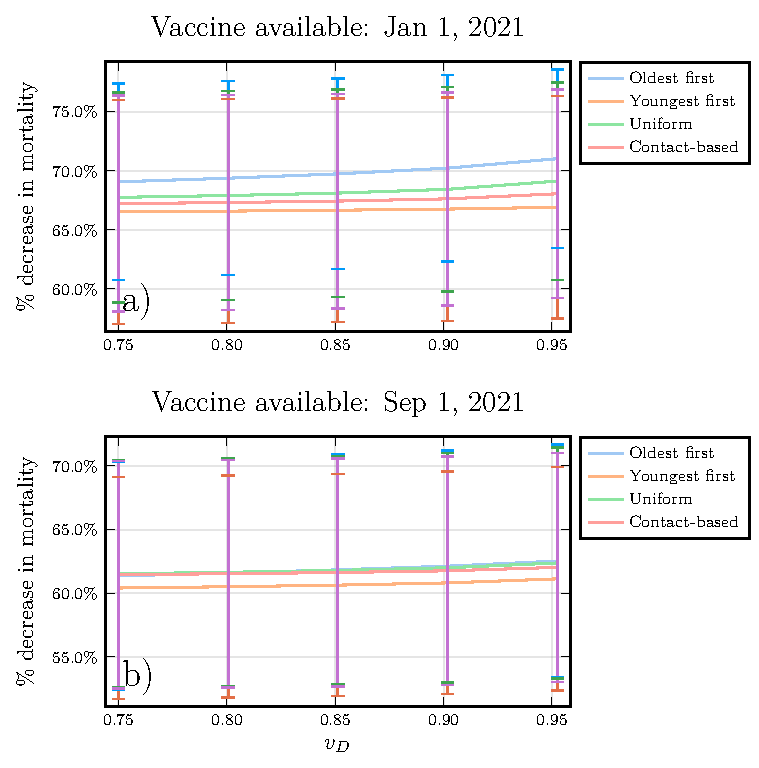
\includegraphics[width = 14 cm]{appendices/FigureS23.pdf}
    \caption{\textbf{Sensitivity analysis for the scenario where efficacy against disease $v^D$ is not the same as efficacy against transmission $v^T$.} Subpanels show percentage reduction in mortality for the four stategies versus $v^D$ when $v^T=0.75$ but $v^D$ ranges from $0.75$ to $0.95$, for January and September availability.  Other parameter values as in Table S1.  Note that mortality in this plot is computed from March 15, 2020 to March 14, 2025.}
    \label{s23}
    \end{figure}
    
    \clearpage 
    
    
    \begin{figure}[H]
    \centering
    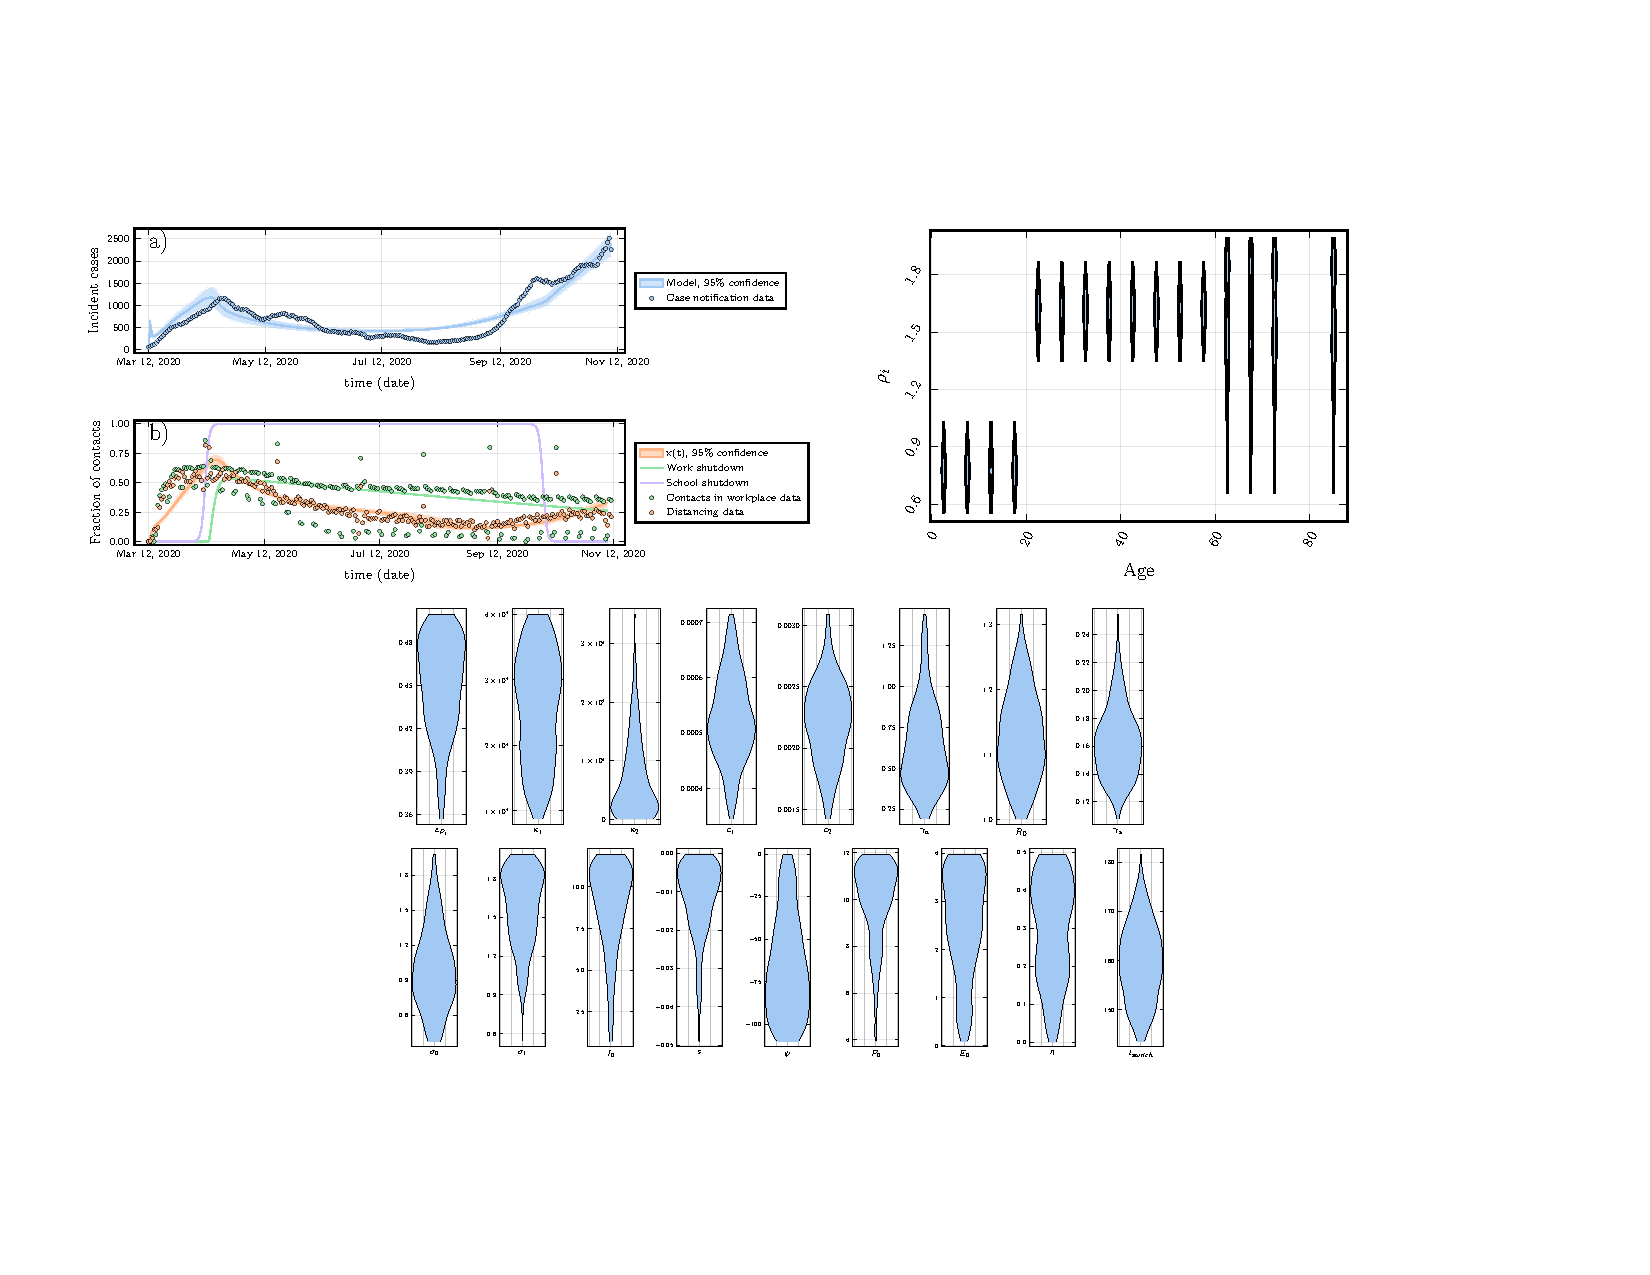
\includegraphics[width = 16 cm]{appendices/FigureS24.pdf}
    \caption{\textbf{Posterior parameter distributions and model outputs for more stringent particle filtering criteria under Bayesian particle filtering algorithm.} Top left panel shows (a) COVID-19 case incidence by date of report in Ontario, 7-day running average (circles) and ascertained case incidence from best fitting models (lines). (b) Percentage change from baseline in time spent at retail and recreation destinations (orange circles) and at workplaces (green circles) from Google mobility data, and proportion of the population x adhering to NPIs (orange line) and workplace shutdown curve (green line) from fitted model.  Top right panel shows posterior parameter distribution for age-specific susceptibility modifier, $\rho_i$ . Bottom panel shows other posterior parameter distributions. Other parameter values as in Appendix, pp. 1-11.}
    \label{s24}
    \end{figure}
    
    \begin{figure}[H]
    \centering
    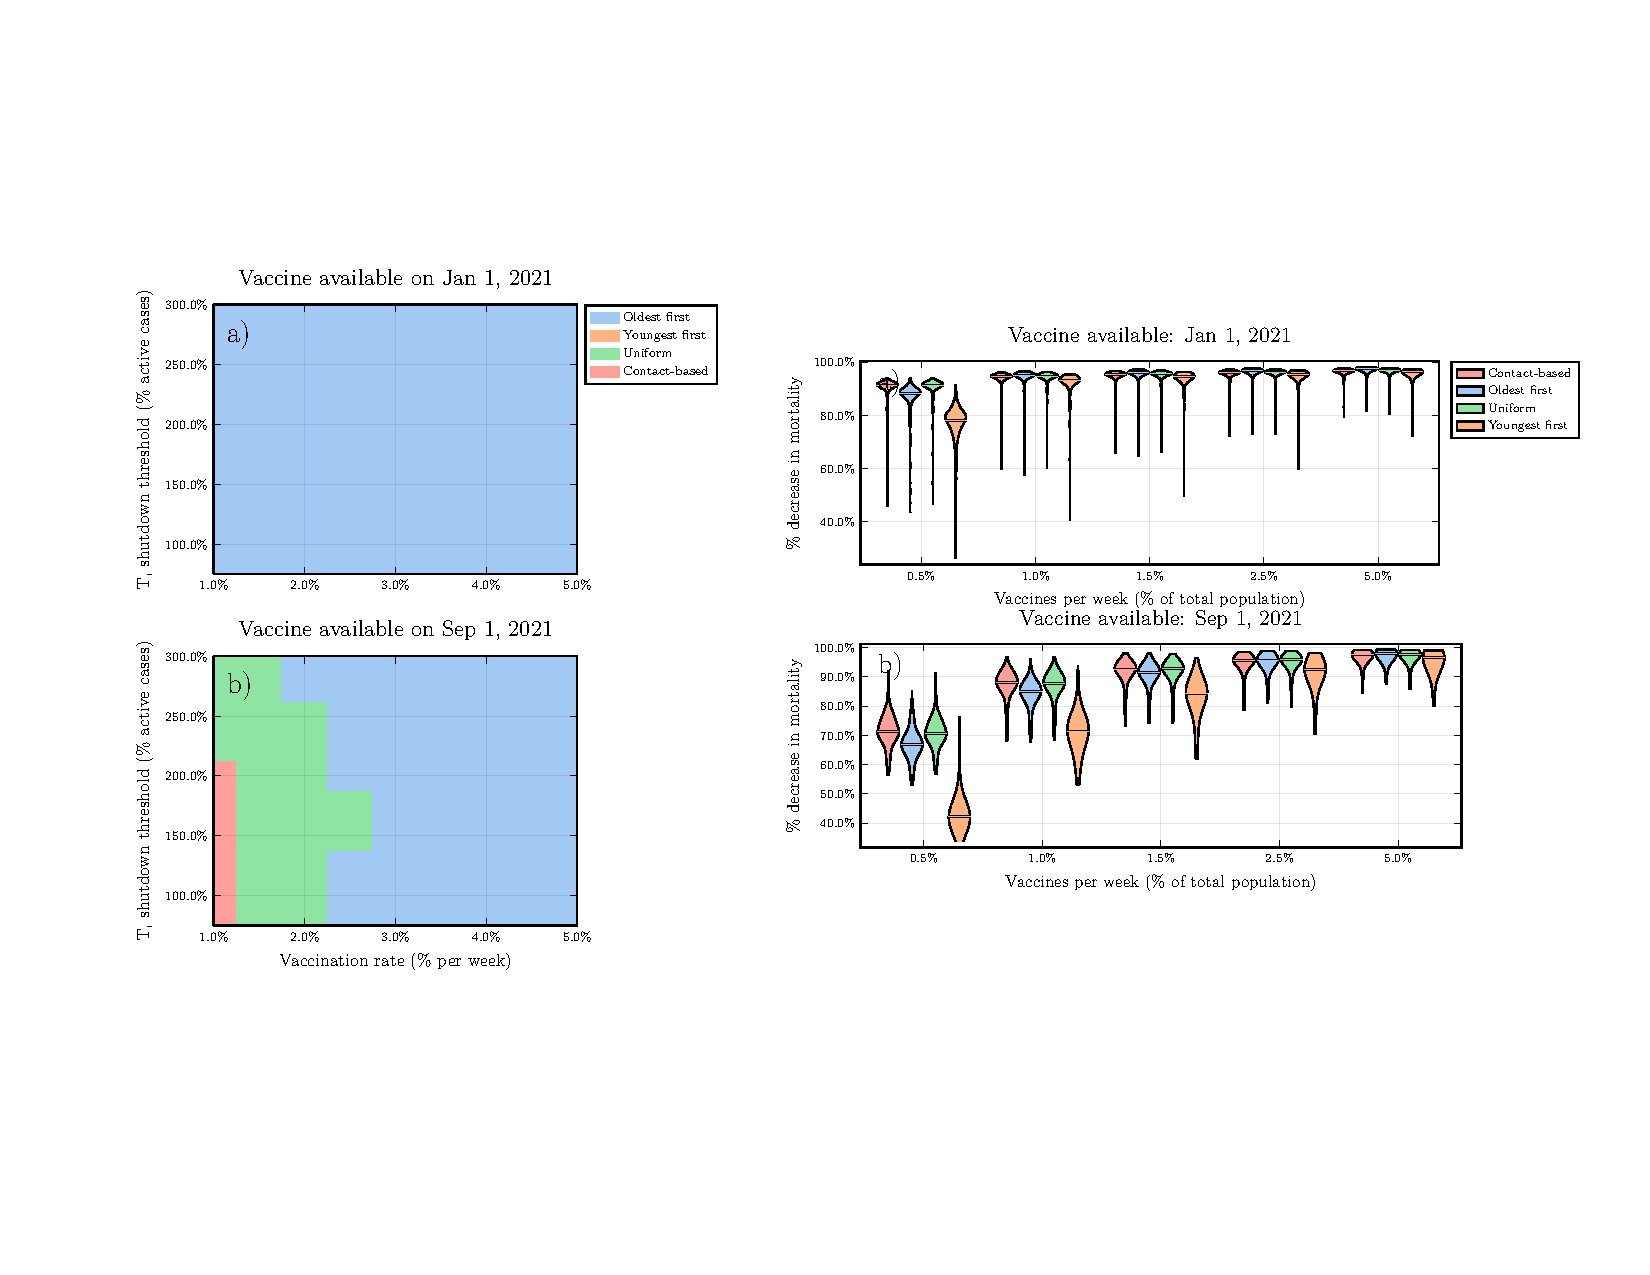
\includegraphics[width = 16 cm]{appendices/FigureS25.pdf}
    \caption{\textbf{Sensitivity analysis for more stringent particle filtering criteria under Bayesian particle filtering algorithm.} Subpanels are parameter planes for January and September availability showing the vaccination strategy that reduces COVID-19 mortality the most as a function of $T$ and $\psi_0$ (left) and violin plots showing percentage reduction in mortality (right).  Horizontal lines represent median values of posterior model projections. Shutdown threshold T=200 \% and other parameter values in Appendix, pp. 1-11. Percentage reductions are relative to no vaccination. Projected number of deaths in the absence of vaccination was 72,000 (95\% credible interval: 40,000 to 122,000) from January 1, 2021 to March 14, 2025 for (a) and 60,000 (95\% credible interval: 31,000 to 108,000) from September 1, 2021 to March 14, 2025 for (b).  Ontario Population size: 14.6 million.}
    \label{s25}
    \end{figure}
    
    \clearpage 
    
    \begin{figure}[H]
    \centering
    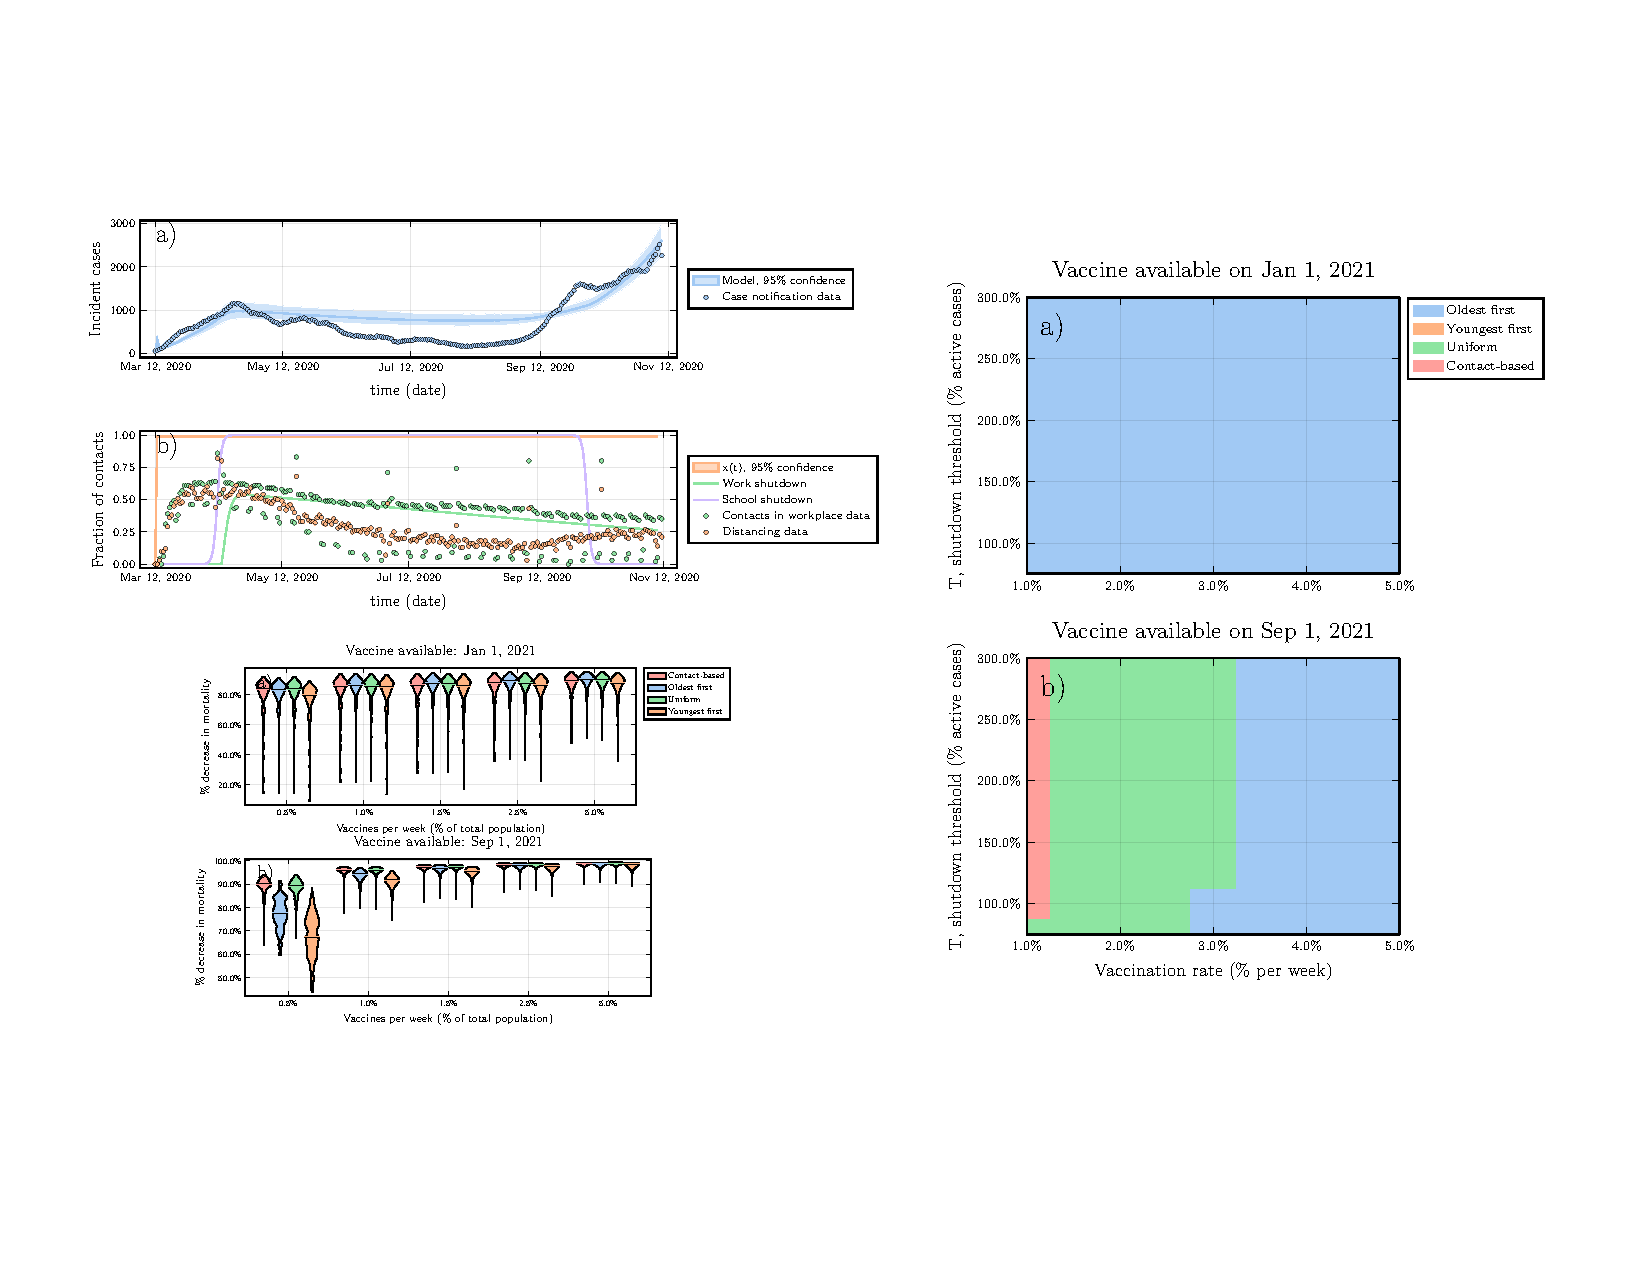
\includegraphics[width = 16 cm]{appendices/FigureS26.pdf}
    \caption{\textbf{Model fit to data and baseline projections of mortality reductions under the four vaccine strategies, when behaviour is held constant over time.} Top left: a) COVID-19 case incidence by date of report in Ontario, 7-day running average (circles) and ascertained case incidence from best fitting models (lines). (b) Percentage change from baseline in time spent at retail and recreation destinations (orange circles) and at workplaces (green circles) from Google mobility data, and proportion of the population x adhering to NPIs (orange line) and workplace shutdown curve (green line) from fitted model. Bottom left: Violin plots of the percent reduction in mortality under the four vaccine strategies, relative to no vaccination, as a function of the vaccination rate ψ0, for (a) January and (b) September 2021 availability. Horizontal lines represent median values of posterior model projections. Shutdown threshold T=200\%. Percentage reductions are relative to no vaccination. Projected number of deaths in the absence of vaccination was 72,000 (95\% credible interval: 40,000 to 122,000) from January 1, 2021 to March 14, 2025 for (a) and 60,000 (95\% credible interval: 31,000 to 108,000) from September 1, 2021 to March 14, 2025 for (b).  Ontario Population size: 14.6 million.  Right:  Each parameter combination on the plane is colour coded according to which of the four strategies prevented the most deaths, on average across all model realizations, for (a) January and (b) September 2021 availability. Other parameter values in Appendix, pp. 1-11.}
    \label{s26}
    \end{figure}
    
    \clearpage 
    
    \begin{figure}[H]
    \centering
    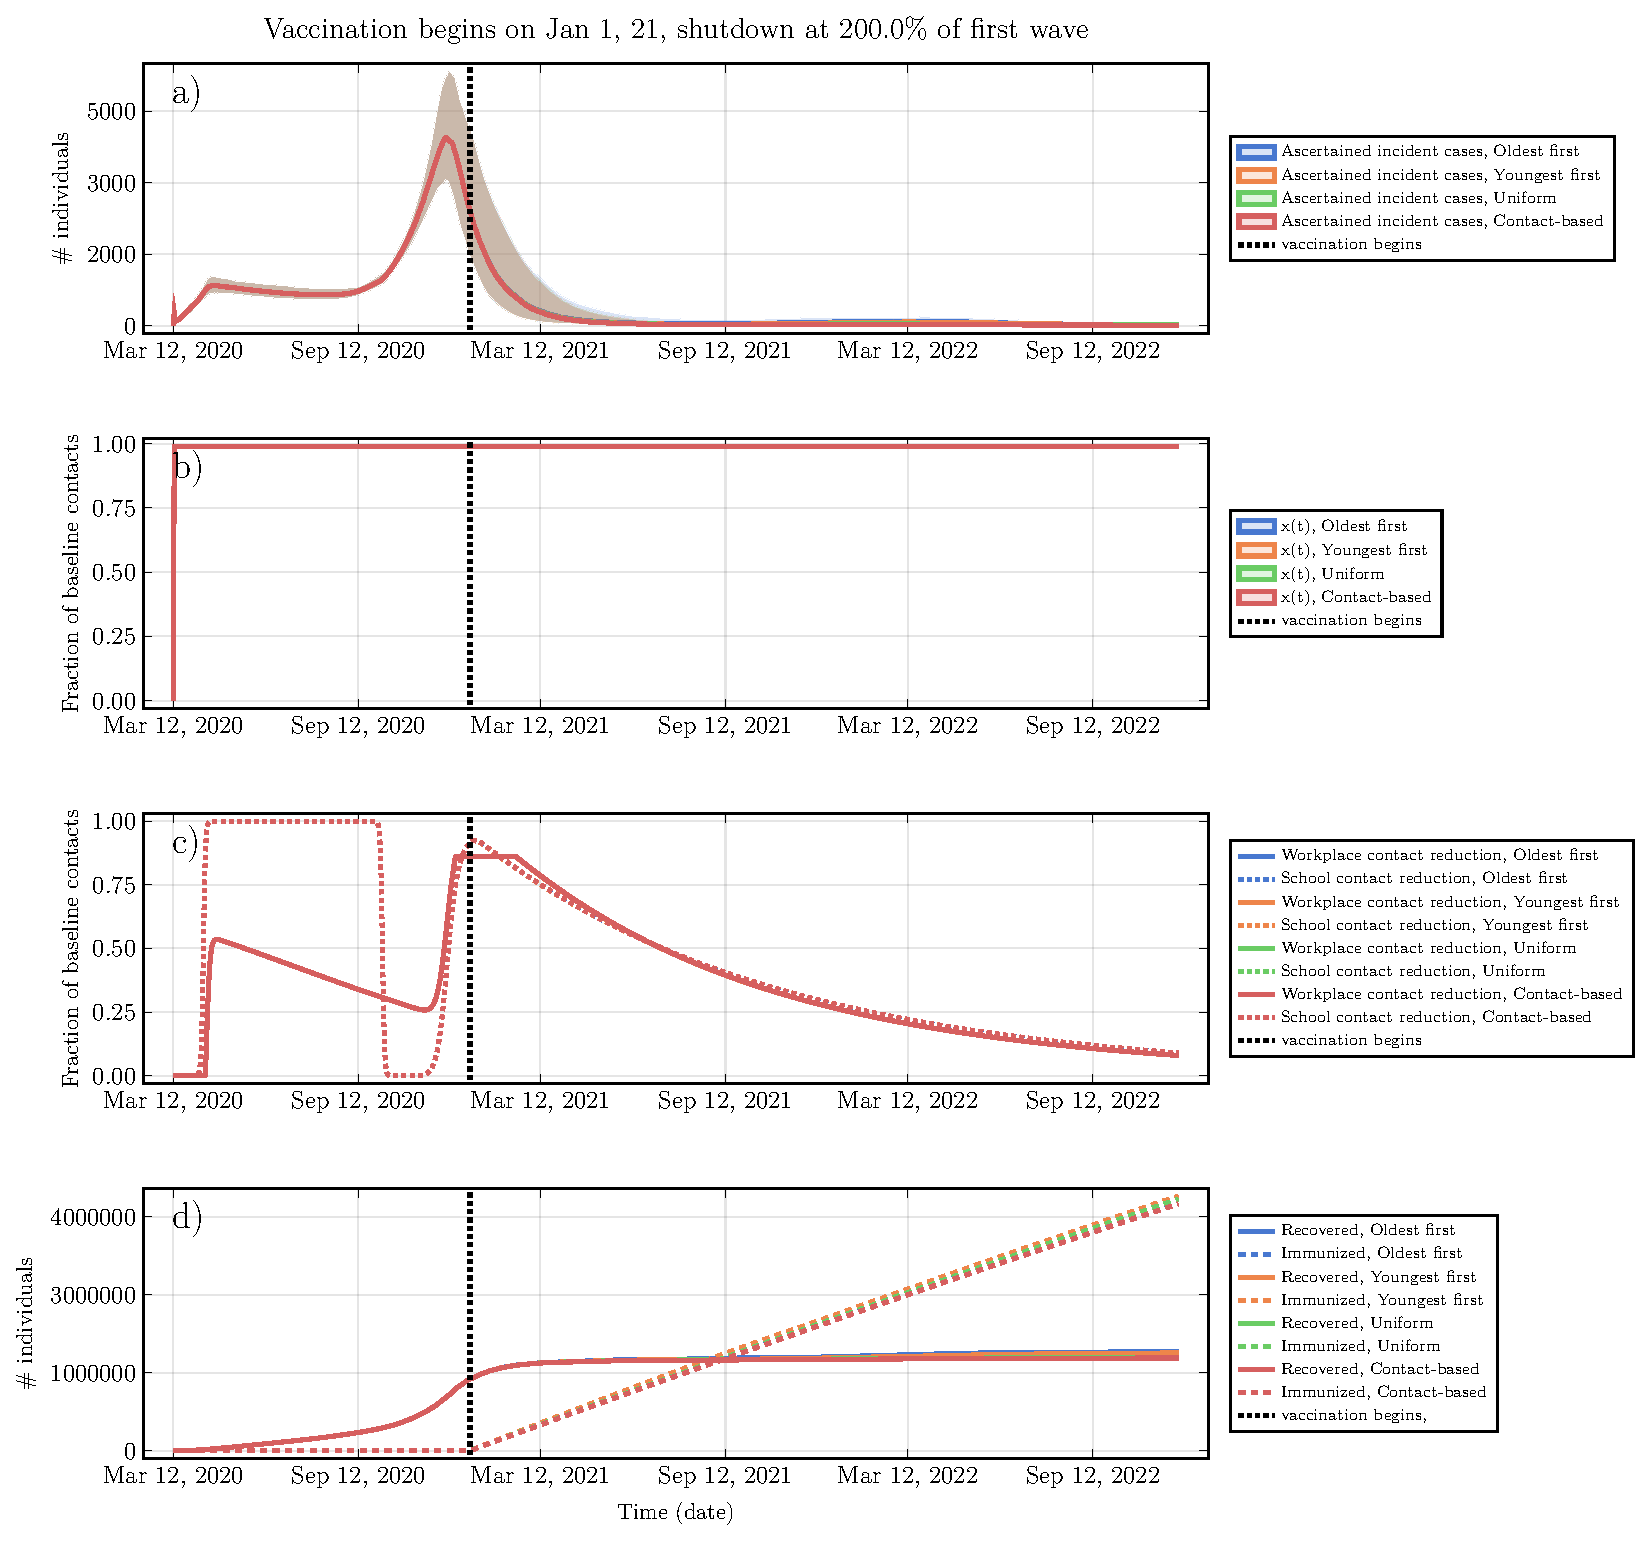
\includegraphics[width = 16 cm]{appendices/FigureS27.pdf}
    \caption{\textbf{Epidemic dynamics and social dynamics for both NPI adherence and vaccinating behaviour, when behaviour is held constant over time.} (a) Ascertained incident COVID-19 cases, (b) proportion $x$ of the population practicing NPIs, (c) Intensity of school and workplace closure, (d) percentage of population with natural or vaccine-derived immunity versus time. $T=200 \%$, $\psi_0=0.5 \%$ per week, vaccine available in January 2021. Other parameters are in Table \ref{tab:params}.}
    \label{s27}
    \end{figure}
    


\begin{figure}
    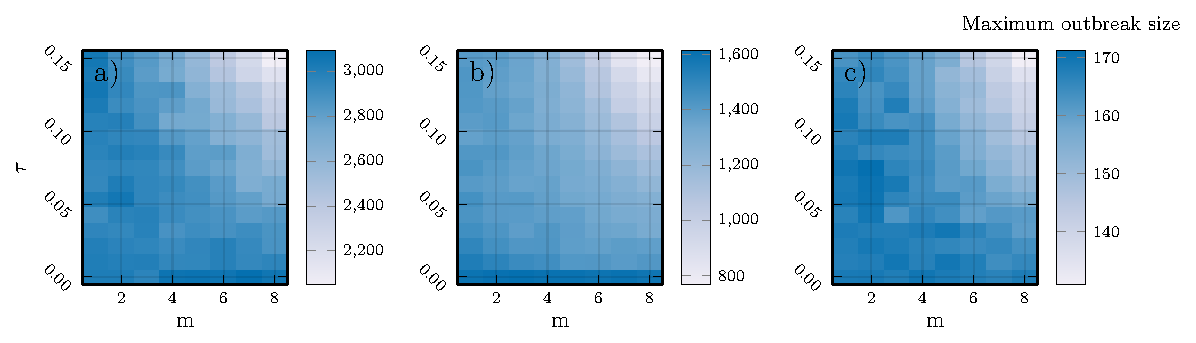
\includegraphics[width=\textwidth]{appendices/data_base_fig.pdf}
    \caption{Maximum MPB infestation size within 500 year period, under FTP with respect to $\tau$ fraction of $m$ juvenile stands cleared. a) ($\alpha_1 = 0.02$, $\alpha_2 = 0.0025$), b) ($\alpha_1 = 0.01$, $\alpha_2 = 0.006$.), c)($\alpha_1 = 0.03$, $\alpha_2 = 0.0012$.)}
    \label{beetle_pop_yearly}
  \end{figure}
  
  \begin{figure}
    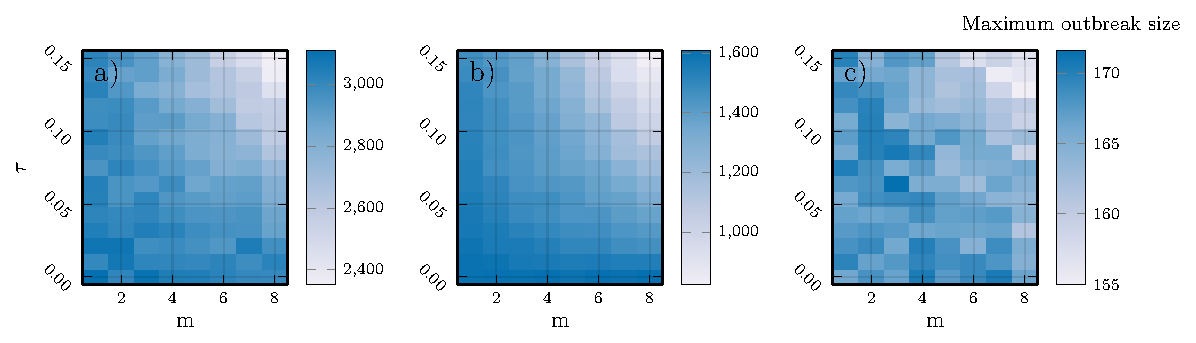
\includegraphics[width=\textwidth]{appendices/data_five_year_trim_fig.pdf}
    \caption{Maximum MPB infestation size within 500 year period, under FTP with respect to $\tau$ fraction of $m$ juvenile stands cleared, conducted every \emph{five} years. a)($\alpha_1 = 0.02$, $\alpha_2 = 0.0025$), b)($\alpha_1 = 0.01$, $\alpha_2 = 0.006$.), c)($\alpha_1 = 0.03$, $\alpha_2 = 0.0012$.)}
    \label{beetle_pop_five_years}
  \end{figure}
  
  \begin{figure}
    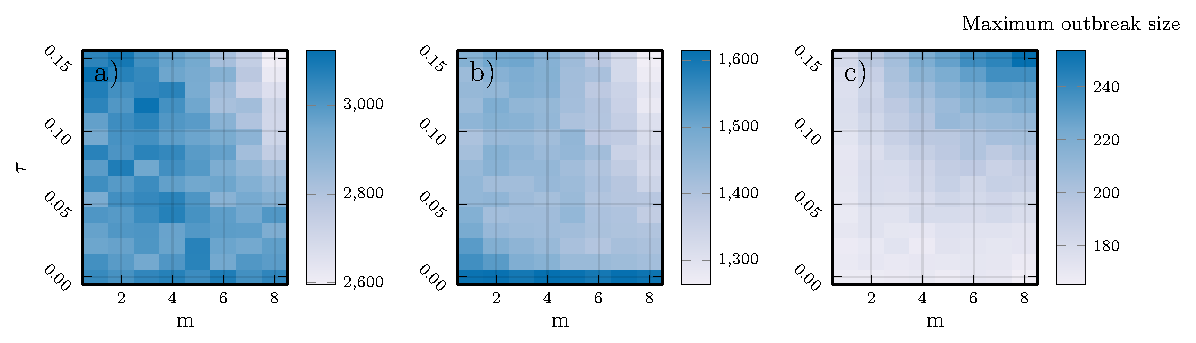
\includegraphics[width=\textwidth]{appendices/data_yearly_burn_fig.pdf}
    \caption{Maximum MPB infestation size within 500 year period, under CBP with respect to $\tau$ fraction of $m$ juvenile stands cleared, conducted each year. a)($\alpha_1 = 0.02$, $\alpha_2 = 0.0025$), b) ($\alpha_1 = 0.01$, $\alpha_2 = 0.006$.), c) ($\alpha_1 = 0.03$, $\alpha_2 = 0.0012$.)}
    \label{CBP_five_years}
  \end{figure}


%----------------------------------------------------------------------
\end{document} % end of logical document
